\chapter{Stride}
\label{chapter:stride}
This chapter describes the main subject of this thesis, which is the individual-based simulator for the transmission of infectious diseases or Stride for short. Before diving into pseudo code, we will explain the reasoning behind it and discuss the most important concepts. Furthermore, we lay out and examine its workings, as well as the data that is being used.

\section{Key aspects}
Before diving into the details and code of Stride, we need a better understanding of the model. This is gained by first figuring out what the most important concepts of Stride were when it was designed, followed by the two most important aspects, namely the individuals and the contact pools. Lastly, the configurations will be discussed since they determine how the model should be run.

\subsection{Core concepts}
Computer models have proven to provide valuable information in the spread of infectious diseases and what results of countermeasures can be \cite{modelling_importance}. The paper in which Stride is presented by Elise Kuylen et al. \cite{stride} states the following:
\begin{quoting}
"Several individual-based models for the transmission of infectious diseases, that take into account heterogeneous social mixing, have already been proposed, but only a few of these, such as FluTE \cite{flute} and FRED \cite{fred} are publicly available as open-source projects."
\end{quoting}
The way they describe Stride is as follows:
\begin{quoting}
"An open-source individual-based model for infectious disease transmission, which explicitly takes into account age, type of day and context when simulating social contacts."
\end{quoting}
Stride's main goal is thus to give a more accurate representation of transmission of infectious diseases by making the simulations resemble more closely to real life. The way Stride does this is by heavily focusing on the social contacts and the different aspects that influence these, since social contacts are crucial for infectious disease transmission \cite{stride}.

\subsubsection{Age}
\label{subsec:age}
The first key aspect of social contacts in Stride is age. The model works on a heterogeneous population in which every individual is different, including their age. In calculating the contacts between people, age has a big impact on who someone meets. Figure \ref{subfig:age_mixing_pattern} shows Stride's resulting age-mixing pattern, which is a representation of the different contact rates based on age. This may seem odd at first, but the explanation behind the results is that people are mainly mixing with people of the same age. The diagonal line between the bottom-left and upper-right corner represents the contact rates between people of the same age, which also has the highest contact rates in each row and column. The bottom left yellow area is the result of children having contact with their peers at school, which also goes for the yellow area in the middle that represents people meeting with their colleagues. It is thus clear that age is a major influential factor in who an individual meets.

\begin{figure}
    \centering
    \subcaptionbox{Age-mixing patterns in which yellow indicates high contact rates and red low contact rates.\label{subfig:age_mixing_pattern}}[.45\textwidth]{
        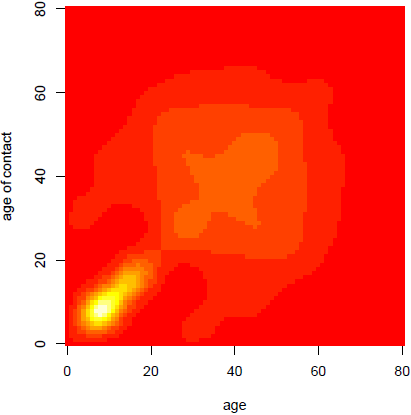
\includegraphics[width=.45\textwidth]{3 - Stride/fig/age-mixing_patterns.png}}
    \hfill
    \subcaptionbox{Number of influenza cases over time using different scenarios regarding the type of days.\label{subfig:type_of_day}}[.45\textwidth]{
        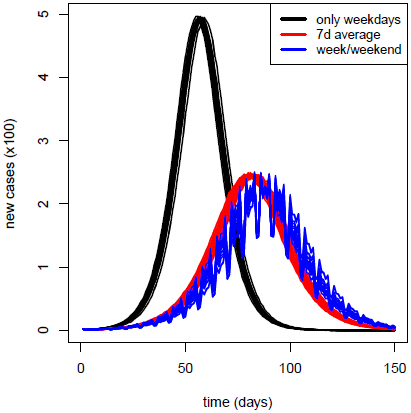
\includegraphics[width=.45\textwidth]{3 - Stride/fig/type_of_days.png}}
    \caption{Stride's social mixing results, copied from \cite{stride}.}
    \label{fig:stride_discussion_results}
\end{figure}

\subsubsection{Type of day}
\label{subsubsec:type_of_day}
Another important aspect Stride takes into account is the different type of days. A simulation in which every day is an average day, differs from more detailed simulations. Stride allows therefore for different type of days to be played out, such as weekdays, weekend days, and holidays. That fact that this is an important feature is confirmed in Figure \ref{subfig:type_of_day}, where the total number of infected cases is much higher when using only weekdays instead of different types of days. Likewise, the peak of number of new cases happens a lot earlier when using only weekdays and is significantly higher.

\subsubsection{Social context}
\label{subsec:social_context}
The last major aspect is the context of a social contact. Just as the age and the type of day, this is yet another very intuitive social trait. The context of contacts in Stride is viewed as the places where people can meet. Generally speaking, when in a household, the network density is a lot higher than at work regardless of age. How Stride handles these different social contexts will become clear during this chapter.

\subsection{Individuals}
\label{subsec:individuals}
Since Stride is an individual-based model, the most important parts are the individuals. Each person is defined by its own characteristics such as their age and health. A person's health status is based on the SEIR model, which is discussed in Section \ref{subsec:seir_model}, and can be either susceptible, exposed, infectious, recovered or vaccinated/immunized. Section \ref{sec:concepts_of_infectious_diseases} explained how people can have different reactions on infections, hence it is a rather important feature for a model to take into account when emulating real life. Therefore, every person's health has its own durations for the different stages of infectious diseases from Section \ref{subsec:stages}. How, when, and where individuals can have contact with one another depends on the contact pools in which each person can be present.

\subsection{Contact pools}
\label{subsec:contact_pools}
A person can be a member of four different \textit{contact pools}. These pools represent the different contexts in which an individual can have contact with someone. People are only able to have contact with members of the same pool who are present at the same time. These types of pools are the household, school or workplace, and two communities. An overview of the pools of an individual is visualised in Figure \ref{fig:pools_overview}, which also shows the days when someone can be present in each pool. An important rule is that an individual can only be a part of one pool per pool type.

\begin{figure}[ht]
    \centering
    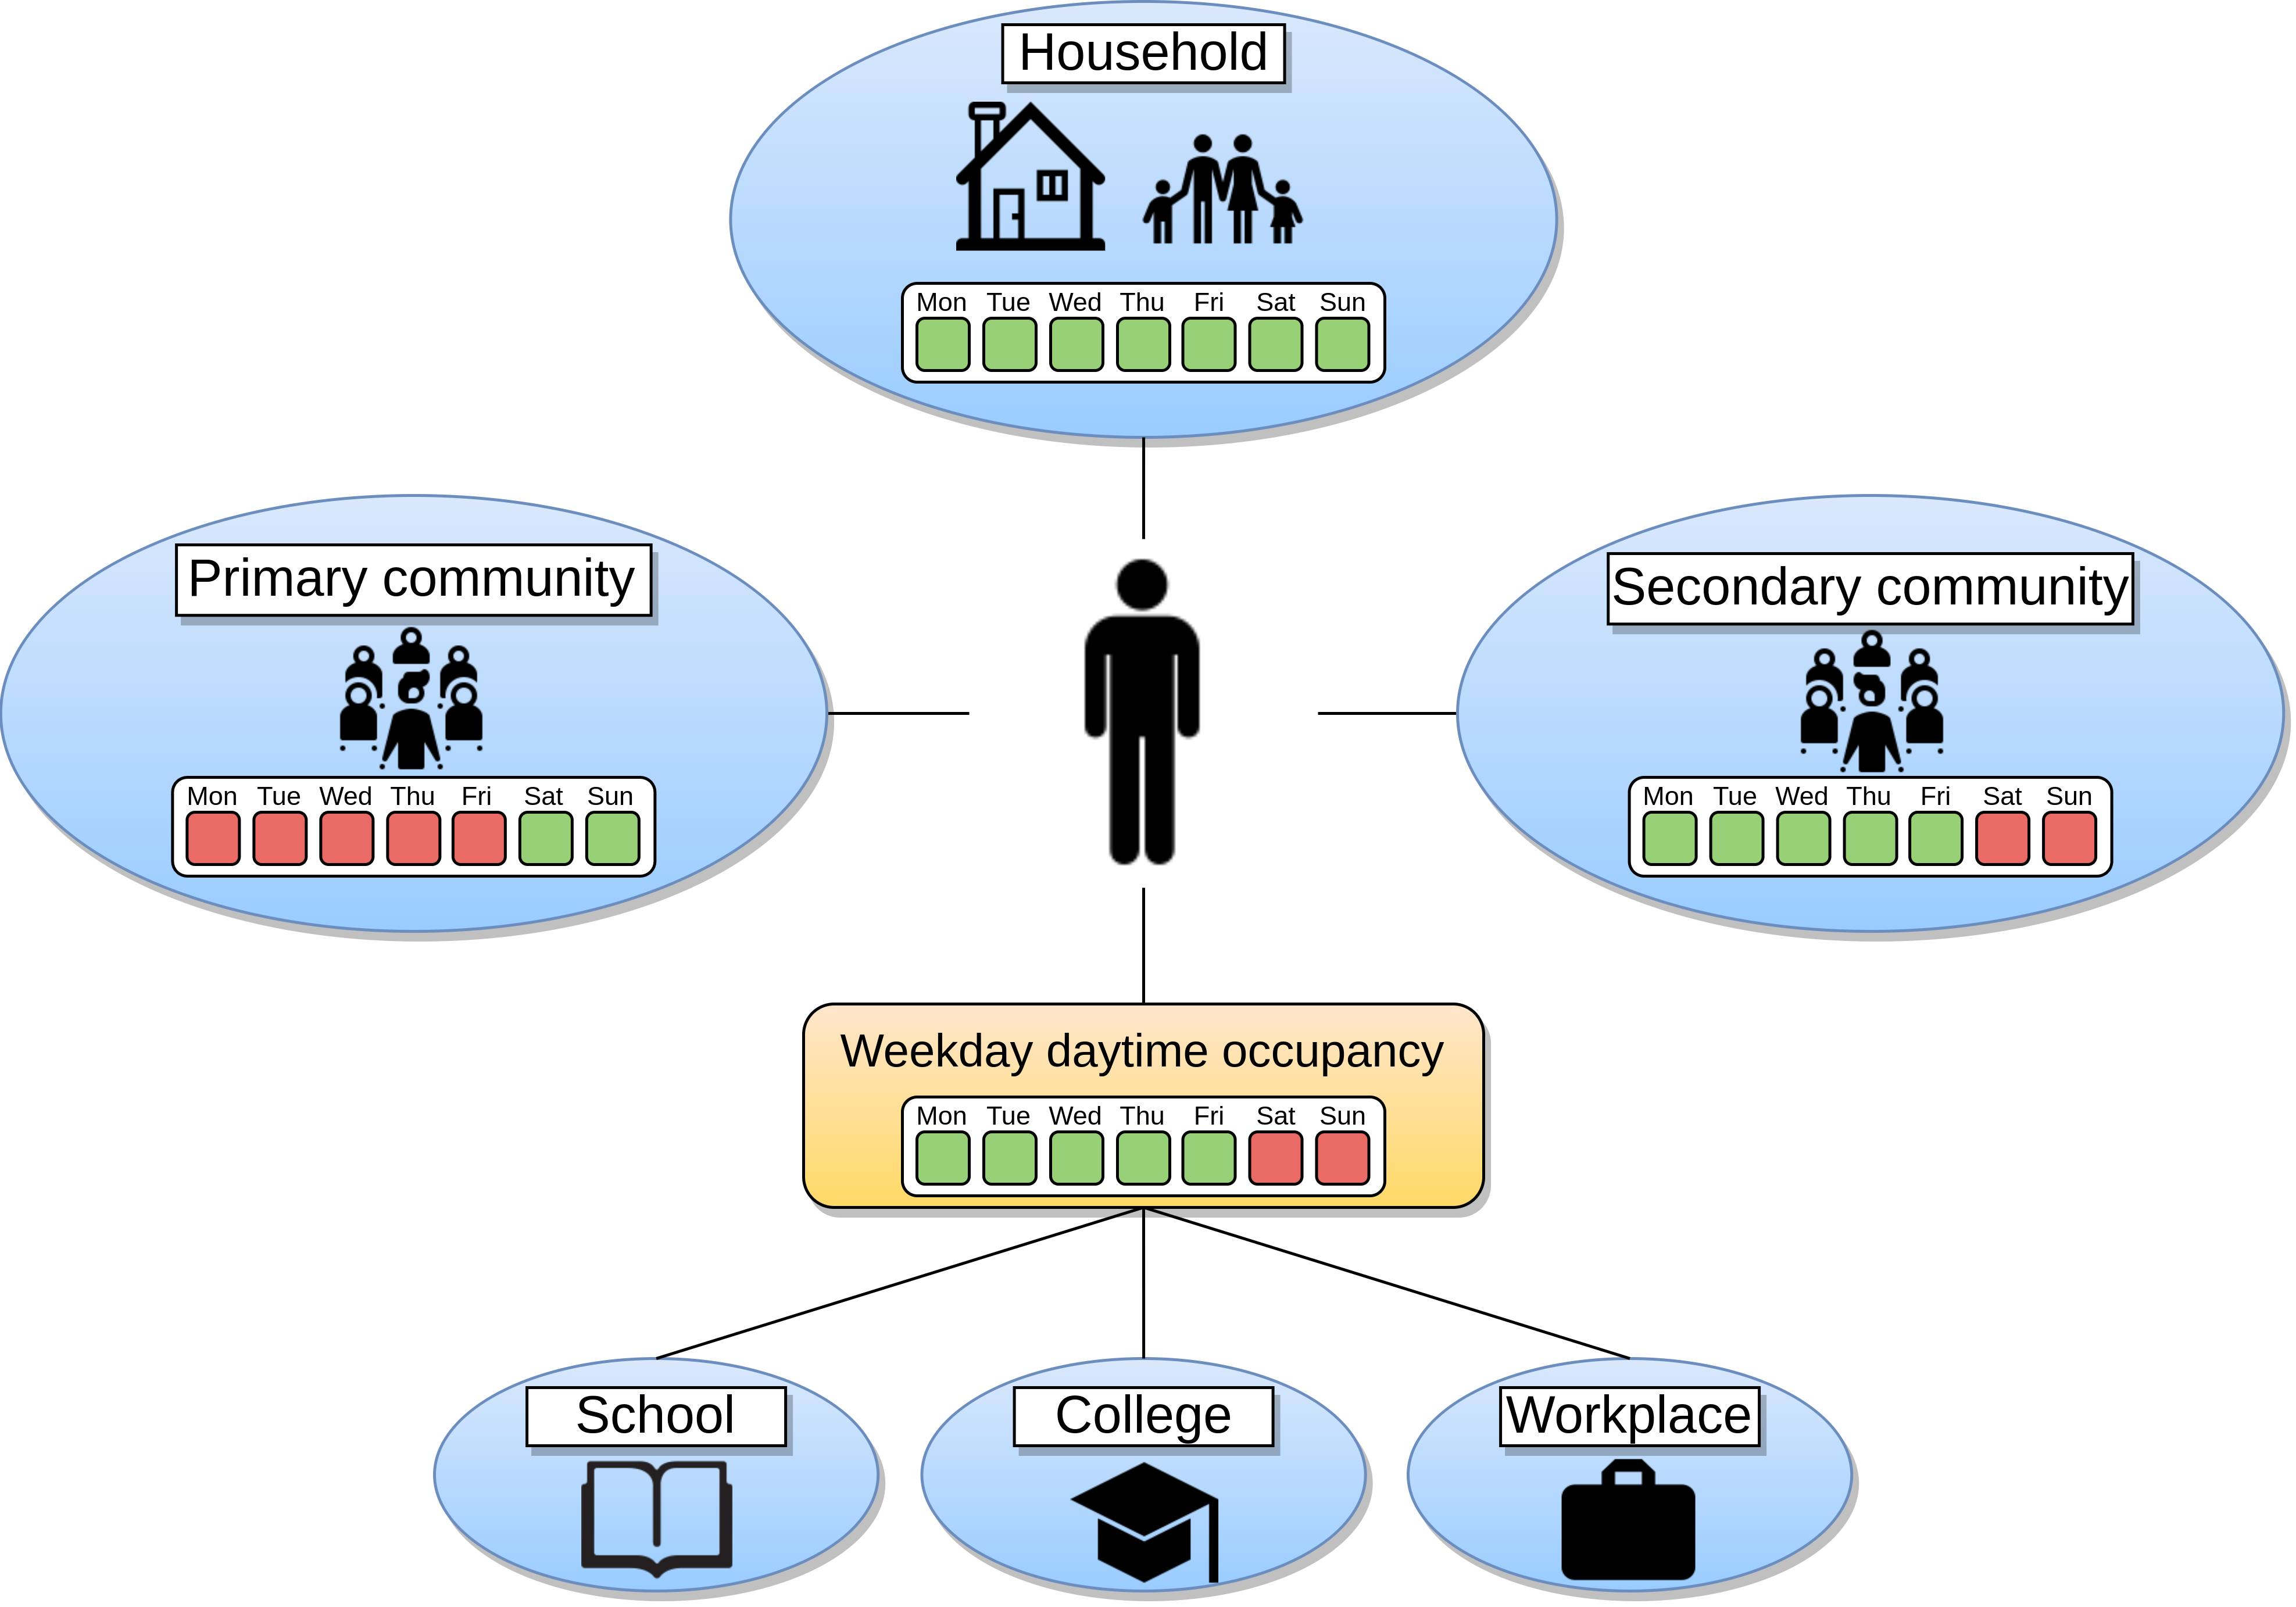
\includegraphics[width=\textwidth]{3 - Stride/fig/Pools_overview.png}
    \caption{Overview of the different type of contact pools. The days colored in green and red in each pool respectively show when an individual can be present or not.}
    \label{fig:pools_overview}
\end{figure}

\subsubsection{Household}
The most straightforward contact pool is the household. Everyone is a member of their own household and will be present in it every day of the week. There is however one exception to this rule, which is when someone is quarantined and is explained in more detail in Section \ref{subsec:pool_presences}.

\subsubsection{School and work}
Of the four types of pools someone can be a part of, there is one type which is not the same for everyone and that is the contact pool that represents an average individual's daytime occupation on a weekday. Just like in real life, what people do during a regular weekday is different for every person: children go to school and adults go to work. Following this logic, individuals younger than 18 years old should be a member of a school-pool and those 18 years and older of a work-pool. This might already be a solid representation for a model, but Stride makes a few extra distinctions here:
\begin{itemize}
    \item Children or young adults, which are people younger than 23 years old, do have a school contact pool, but these pools do not only consist of these people. Schools also need teachers who are of course adults. These teacher individuals are therefore not a part of a workplace contact pool, but instead of a school contact pool.
    \item Another distinction that can be made is the different types of school. This can be done in various ways, but Stride only separates K-12 schools and colleges. K-12 schools describe all the different types of education up until the age of 18 and colleges only contain (young) adults. Obviously, the school contact pools of the teachers and professors also make this distinction since they are in the same pool as their students.
    \item The workplace is the only pool of which an individual is not required to be a part of. A large part of the society in real life does not have a job or is retired. The individuals portraying these people are thus only a member of three contact pools.
\end{itemize}
The days when people can be present in their school or workplace pool are the weekdays from Monday to Friday, so weekend jobs do not exist in the simulation. However, as Section \ref{subsubsec:type_of_day} explained that Stride takes different types of days into consideration, the holidays cause for people to skip their school or workplace pools on these days. People who feel ill also typically don't go to school or their work, so they might then also not appear in their contact pool as will be seen in Section \ref{subsec:pool_presences}.

\subsubsection{Communities}
The last types of contact pools are the communities, of which there are two: the primary and secondary community. These pools represent the times when someone is not at school or work, and not at home. They can be described as the places and people someone meets in their spare time such as when practising a sport or other hobbies. Those pools represent the same concept, but do not occur at the same time or consist of the same people. The primary community is used for the contacts that are being made in the weekend and on holidays thus people can only be present in them on Saturday, Sunday and on holidays. Correspondingly, the secondary community represents the people someone can meet on a regular weekday outside of their school or workplace pool. Just as someone who feels ill will not go to school or work, they can also decide to stay at home and not attend their primary and secondary community.

\subsection{Configurations}
\label{subsec:configurations}
The previously mentioned aspects give more information about the model itself. How the model must be used in a simulation is decided by the various customisable configurations. Covering every single configuration would be a little otiose, so only the ones that are considered relevant will be explained.

\subsubsection{Population}
Sections \ref{subsec:individuals} and \ref{subsec:contact_pools} showed how individuals are being represented and how they are divided in contact pools where they can have contact with each other. These individuals and their contact pools are configured in a population file which contains a row for every individual. Such a row consists of non-negative integers representing the individual's age and the ID of every pool type as follows:
$$\textrm{(\textbf{age}, \textbf{household}, \textbf{school}, \textbf{work}, \textbf{primary\_community}, \textbf{secondary\_community})}$$
Since not everyone has to be a member of a school or workplace contact pool, it is possible for these values to be zero, indicating that they do not belong in one.

\subsubsection{Holidays}
As stated in Section \ref{subsubsec:type_of_day}, Stride makes a distinction between the type of days. Next to weekdays and weekend days, holidays are also being accounted for when deciding what kind of day the model has to simulate. These holidays are presented in a file that contains the information of all the days that have to be treated different than usual. This can be as detailed as needed and allows for distinctions to be made. There are for example days that are a national holiday and thus result in everyone not going to school or work (and their secondary community), but there are also holidays that only apply to schools such as summer break so that adults (not teachers) still need to go to work. Another similar example in Belgium is that colleges start somewhere mid September while K-12 schools start the first of September. In the holidays configuration file this is made possible by defining the ages to which a holiday applies.

\subsubsection{Disease characteristics}
Because the purpose of Stride is to enable the analysis of multiple infectious diseases, it needs a generic disease configuration file which describes the characteristics of the disease. This gives the possibility to simulate any disease on the basis of a couple traits. These traits consist of the basic reproduction number\footnote{Simplified explanation: the average number of people someone infects, which describes the infectiousness of a disease.}, the probabilities of being symptomatic or asymptomatic, how long someone can be infectious, etc.

\subsubsection{Event logging}
Subsequent sections will explain how Stride gives the possibility to run faster at the expense of generating less information. The main rule that defines this behaviour is the event logging rule. It determines what type of events need to be logged, such as the transmissions and contacts. The reason for this to have such an impact is that when contacts need to be logged, the model needs to evaluate every possible contact. If only transmissions need to be logged, it suffices to only calculate the transmissions instead of every possible contact. How this effects the model will become clear in Section \ref{subsec:contacts_and_transmissions}.

\subsubsection{Age contact matrix}
By now it is known how individuals and their contact pools are presented. These pools represent different social contexts in which people can have contact with each other. How people interact with one another in every pool is given by the age contact matrix file. This file contains a matrix with the probabilities of two people having contact with respect to their age and the pool type in which they find themselves in. Passing this matrix on to the simulation instead of defining the probabilities in the code, allows for flexible and customisable usage. The details of how this matrix is being used is described in Section \ref{subsec:contact_matrix}.

\subsubsection{Numerical values}
At last, there are various configuration values that are plain numerals. For example the number of days that the model has to simulate, the date at which the simulation has to start, or the number of infected and immune people at the start. There is also a possibility for multi-threading by configuring the number of threads that have to be used, which will be talked about further along this chapter.

\section{Simulation}
\label{sec:simulation}
The next step in gaining insight into Stride is to figure out the simulation. This section will thoroughly explain how the model works and every important part will be covered in detail. A conceptual overview of the simulation flow with its most important components is illustrated in Figure \ref{fig:simulation_flow}. Stride begins by initialising the simulation, which is explained in Section \ref{subsec:initialisation}. Then the simulation commences at the starting date, moving forward in discrete time-steps of one day until the configured number of days have been processed. All of these days consist of the same pattern which is the following:
\begin{enumerate}
    \item Update the health status of every individual (Section \ref{subsec:health_status_update}).
    \item While updating everyone's health, also determine in which pool they will be present (Section \ref{subsec:pool_presences}).
    \item There is a possibility to perform contact tracing if this is set to be active (Section \ref{subsec:contact_tracing}).
    \item Make calculations to determine who has contact with each other and who gets infected (Section \ref{subsec:contacts_and_transmissions}).
\end{enumerate}
There is an additional step, universal testing, which will not be talked about in this thesis, because it was added after the start of the thesis and thus has not been examined. This testing step is similar to the contact tracing step, which is a very small part of the simulation that comes right after the contact tracing step and, as will be discussed in Section \ref{subsec:performance}, is therefore insignificant.

\begin{figure}
    \centering
    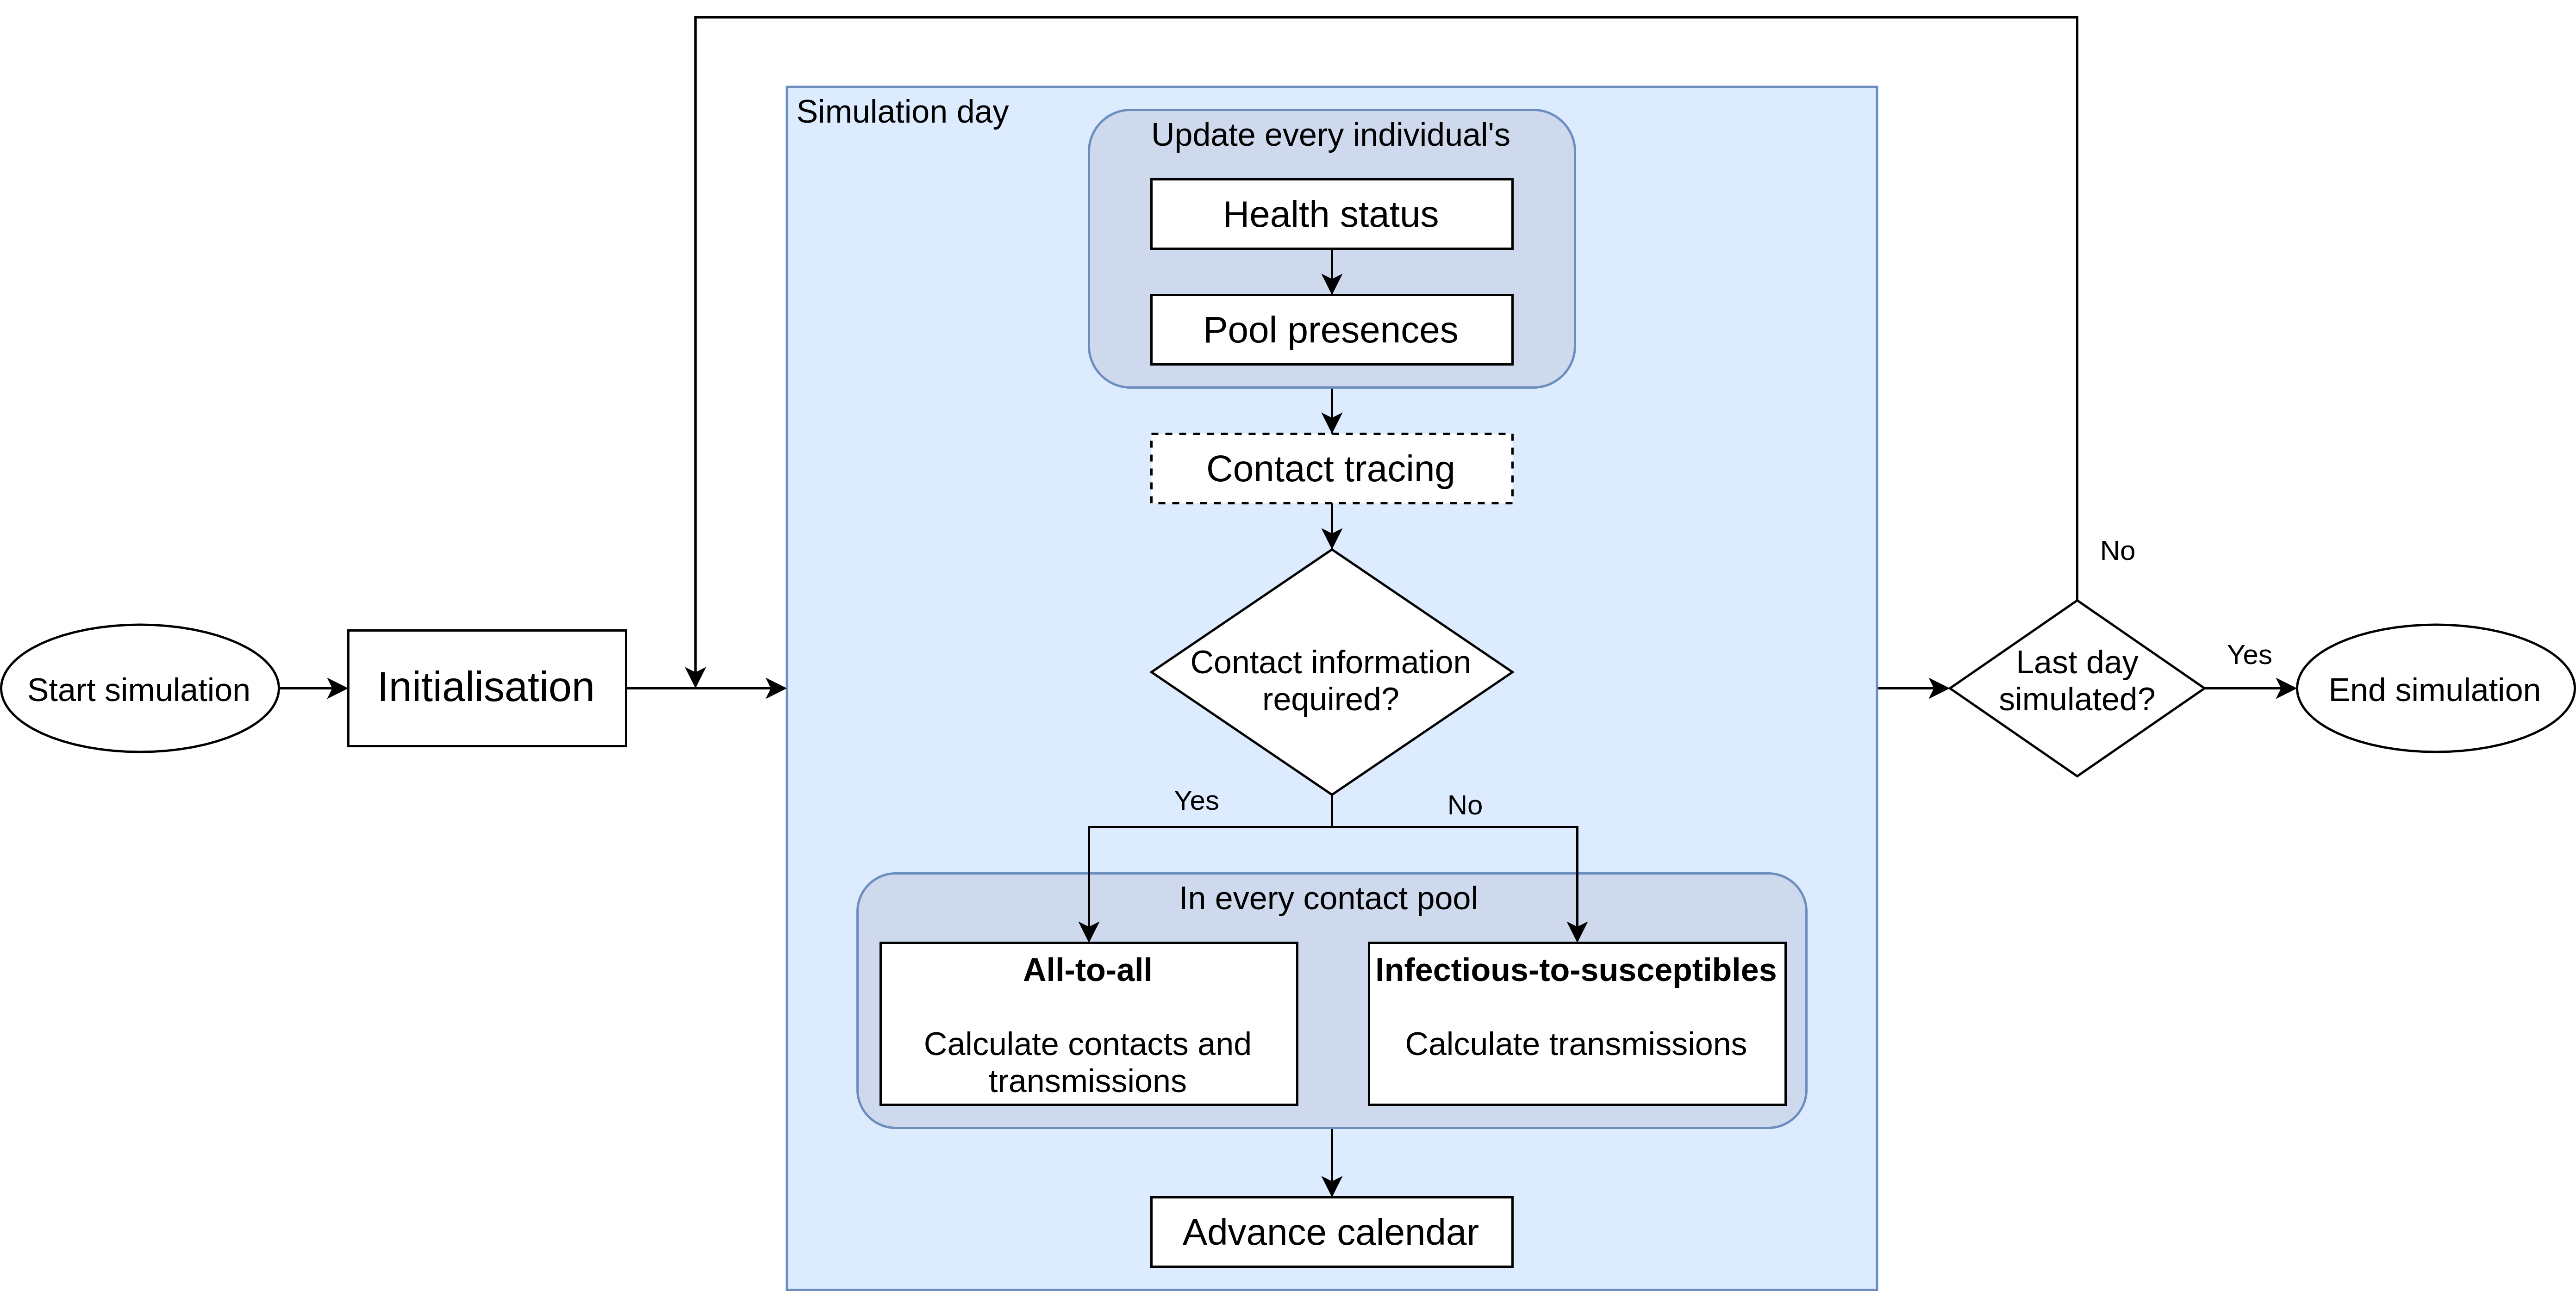
\includegraphics[width=\textwidth]{3 - Stride/fig/high-level_flow.png}
    \caption{Conceptual overview of a Stride simulation.}
    \label{fig:simulation_flow}
\end{figure}

\subsection{Initialisation}
\label{subsec:initialisation}
The initial step of the model is the initialisation, which uses the configurations from Section \ref{subsec:configurations} to set up all the necessary segments before starting the simulation. The first segment that gets initialised is the random number generator manager, which handles all the random numbers and distributions. Next is the population that gets created by generating every individual one by one from the population file, followed by the construction of all the contact pools. Then the calendar is built with the holidays file and the given start date, after which most of the numerical configuration values get processed. Thereafter are the contact matrix and disease characteristics read in and stored.
\\\\
The last step in the initialisation process is to `seed' all the random elements of the simulation. Individuals need to behave in different ways, not only regarding contacts, but also regarding the disease. Every individual's health therefore gets randomly created to determine how long the different stages of the disease will be, which are discussed in Section \ref{subsec:stages}, and whether they will be symptomatic or not. The other seeding that gets done is randomly selecting the individuals that will be infected or immune at the start of the simulation.

\subsection{Health status update}
\label{subsec:health_status_update}
When an individual has not been infected, this step is skipped because their health status does not change then. If someone is infected, however, the simulator will look at their health characteristics that were randomly assigned in the initialisation. On the basis of these characteristics, it determines how the person's health will be in the upcoming day. The different outcomes are that the person becomes or remains infectious, symptomatic, infectious and symptomatic, or that the infection stops.

\subsection{Pool presences}
\label{subsec:pool_presences}
We now know that individuals belong to a pool and can be present or not, but not how this is stored by our model. Every pool is represented by its unique Id, the contact pool type, and its members. It does not keep track of which members are present during the current day. If someone is present or not is only being stored by the person itself. Thus, after a person's health status is updated, their presence in every pool gets evaluated.
\\\\
There are various factors that affect in which pool someone will be present. The most straightforward one is what type of day the current day is, which can be a regular weekday, weekend day, or holiday. When a person is symptomatic and thus feels ill, there is a chance that they will not attend other contact pools except their household.
\\\\
Furthermore, there are factors which are not a part of the standard model, but they are additional features that can be passed on through the configurations. A possible feature is to close schools and workplaces to analyze how it reduces an outbreak. Another element that can be turned on is the ability for a person to work from home and the ability for the `government' of the population to enforce telework. The last non-standard factor is the possibility of quarantine, which translates in the person isolating themselves from every pool, with also being able to be isolated from their household and thus not be present in it.

\subsection{Contact tracing}
\label{subsec:contact_tracing}
If the configurations have indicated that on the current day there will not be contacts traced, then this step is skipped, which also goes for universal testing. For the sake of completeness, this step will only be briefly explained here, because it does not belong to the standard simulation flow. Even when it is incorporated in the simulation, it does not have a big impact on the run time as will be seen in Section \ref{subsec:performance}.
\\\\
The contact tracing step will iterate over the entire population and check who is infected and just recently `felt' symptoms in order to perform the contact tracing, because people who do not feel symptoms would normally not know they are infected. Infected individuals their contacts of the previous days have a probability that they will be traced, which can result in them being put into quarantine. This probability resembles the fact that people in real life do not perfectly know who they have been in contact with and is a numerical configuration value.

\subsection{Contacts and transmissions}
\label{subsec:contacts_and_transmissions}
The final and most important part of a simulated day is calculating every contact and transmission. This is done by iterating over the different pool types to see which pool is active on the current day, so for example the workplace, K-12 school, college, and secondary community contact pools get skipped when it is a national holiday. Then, all the pools of an active pool type are iterated over and get processed to determine the contacts and transmission. There are two algorithms that can be used to do these calculations, for which the choice is made at run time, depending on the need for information about contacts. If information about contacts is needed, the \textsc{All-to-All} algorithm will be selected. When the simulation only needs to handle transmissions and infections, the infectious-to-susceptibles algorithm is used.

\subsubsection{All-to-all}
The first algorithm, of which the pseudo code is shown in Algorithm \ref{alg:all-to-all}, matches everyone of a pool with each other and determines for each member pair if they will have contact and if someone infects the other. Since everyone gets compared with everyone, this algorithm will be called \textsc{All-to-All} from now on. For every member pair in a contact pool, of which both individuals are present, the probability that they have contact is calculated. Then we perform a Bernoulli trial to randomly determine if there is contact, which expresses two different outcomes, success (contact) and failure (no contact), given our contact probability. When contact has been made, the next step is to look at the health statuses of the pair. If one of them is infectious while the other is susceptible, the probability of transmission is calculated. Similar to determining contact, the incident of the infectious person transmitting the disease to the susceptible one is decided by a Bernoulli trial based on the transmission probability. The susceptible person then becomes infected by the infectious one.

\begin{algorithm}
\caption{Pseudo code of the \textsc{All-to-All} algorithm.}
\label{alg:all-to-all}
\begin{algorithmic}[1]
    \Require{$P_{1} \dots P_{N}$}\Comment{All members of the pool}\;
    \Statex
    \For{$i \gets 1$ to $N$}\Comment{Iterate over all members}
        \State $P_{1} \gets P[i]$
        \If{$P_{1}$ not present}
            \State continue to next $i$
        \EndIf
        \For{$j \gets i$ to $N$}\Comment{Iterate over members starting from $i$}
            \State $P_{2} \gets P[j]$
            \If{$P_{2}$ not present}
                \State continue to next $j$
            \EndIf
            \Statex
            \State $C_{prob} \gets$ probability $P_{1}$ and $P_{2}$ have contact
            \If{\Call{BernoulliTrial}{$C_{prob}$}}
                \State Register contact
                \If{$P_{1}$ or $P_{2}$ susceptible and other infectious}
                    \State $T_{prob} \gets$ probability infection happens
                    \If{\Call{BernoulliTrial}{$T_{prob}$}}
                        \State Infect the susceptible one
                    \EndIf
                \EndIf
            \EndIf
        \EndFor
    \EndFor
\end{algorithmic}
\end{algorithm}

\subsubsection{Infectious-to-susceptibles}
Section \ref{subsec:performance} will explain how the \textsc{All-to-All} algorithm becomes a lot slower depending on the number of people in a contact pool. Therefore, an optimised approach has been designed to be a lot quicker in exchange for producing less information. This other algorithm will be called the \textit{infectious-to-susceptibles} (\textsc{Inf-to-Sus} for short), because it only compares every infectious person in a pool with every susceptible one to determine who gets infected. At first, the pool gets sorted based on the health status of every member, which is explained in the next section, and it is counted how many infectious members the pool contains. If there are no infectious people in the pool, the algorithm immediately stops. However, if there are infectious members of the pool, the next step is to match the infectious ones with the susceptibles. For every pair of an infectious and a susceptible person, who are both present, the probability for them to have contact and the probability of transmission is calculated and multiplied with each other. This probability result is then used for a Bernoulli trial to randomly decide if the infectious person infects the susceptible one, after which the susceptible person becomes infected or not. Note that this algorithm only generates information about the transmissions and limits itself to contacts between infectious and susceptible persons. As such, it cannot be used to calculate contacts over the entire population, which the \textsc{All-to-All} method can.

\begin{algorithm}
\caption{Pseudo code of the \textsc{Inf-to-Sus} algorithm.}
\label{alg:inf-to-sus}
\begin{algorithmic}[1]
    \Require{$P_{1} \dots P_{N}$}\Comment{All members of the pool}\;
    \Statex
    \State sort $P[\;]$ on health status \Comment{Explained in Algorithm \ref{alg:health_sorting}}
    \Statex
    \State $N_{inf} \gets$ number of infected members
    \If{$N_{inf} = 0$}
        \State \Return
    \EndIf
    \Statex
    \State $i_{sus} \gets$ index of first susceptible member
    \State $i_{imm} \gets$ index of first immune member
    \Statex
    \For{$i \gets 1$ to $(i_{sus}-1)$}\Comment{Iterate over possible susceptibles}
        \State $P_{1} \gets P[i]$
        \If{$P_{1}$ not present or not infectious}
            \State continue to next $i$
        \EndIf
        \For{$j \gets i_{sus}$ to $(i_{imm}-1)$}\Comment{Iterate over susceptibles}
            \State $P_{2} \gets P[j]$
            \If{$P_{2}$ not present}
                \State continue to next $j$
            \EndIf
            \State $CT_{prob} \gets$ probability of contact AND transmission between $P_{1}$ and $P_{2}$
            \If{\Call{BernoulliTrial}{$CT_{prob}$}}
                \State $P_{1}$ infects $P_{2}$
            \EndIf
        \EndFor
    \EndFor
\end{algorithmic}
\end{algorithm}

\subsubsection{Sorting on health status}
Line 9 of Algorithm \ref{alg:inf-to-sus} may look like it performs a redundant check by confirming that \textit{p1} is infectious, but this is due to the way the contact pools are sorted on line 1. Algorithm \ref{alg:health_sorting} shows the pseudo code of this sortation based on the health statuses. A visual representation of a list of contact pool members before and after sorting on health statuses can be seen in Figure \ref{fig:health_sort}. Everyone who is immune is placed together at the end of the list and the susceptibles are arranged right in front of them. The remaining people with the health status exposed, infected, or recovered are put together with no specific order amongst them. \textsc{Inf-to-Sus} therefore needs to distinguish the infectious from the rest.

\begin{figure}
    \centering
    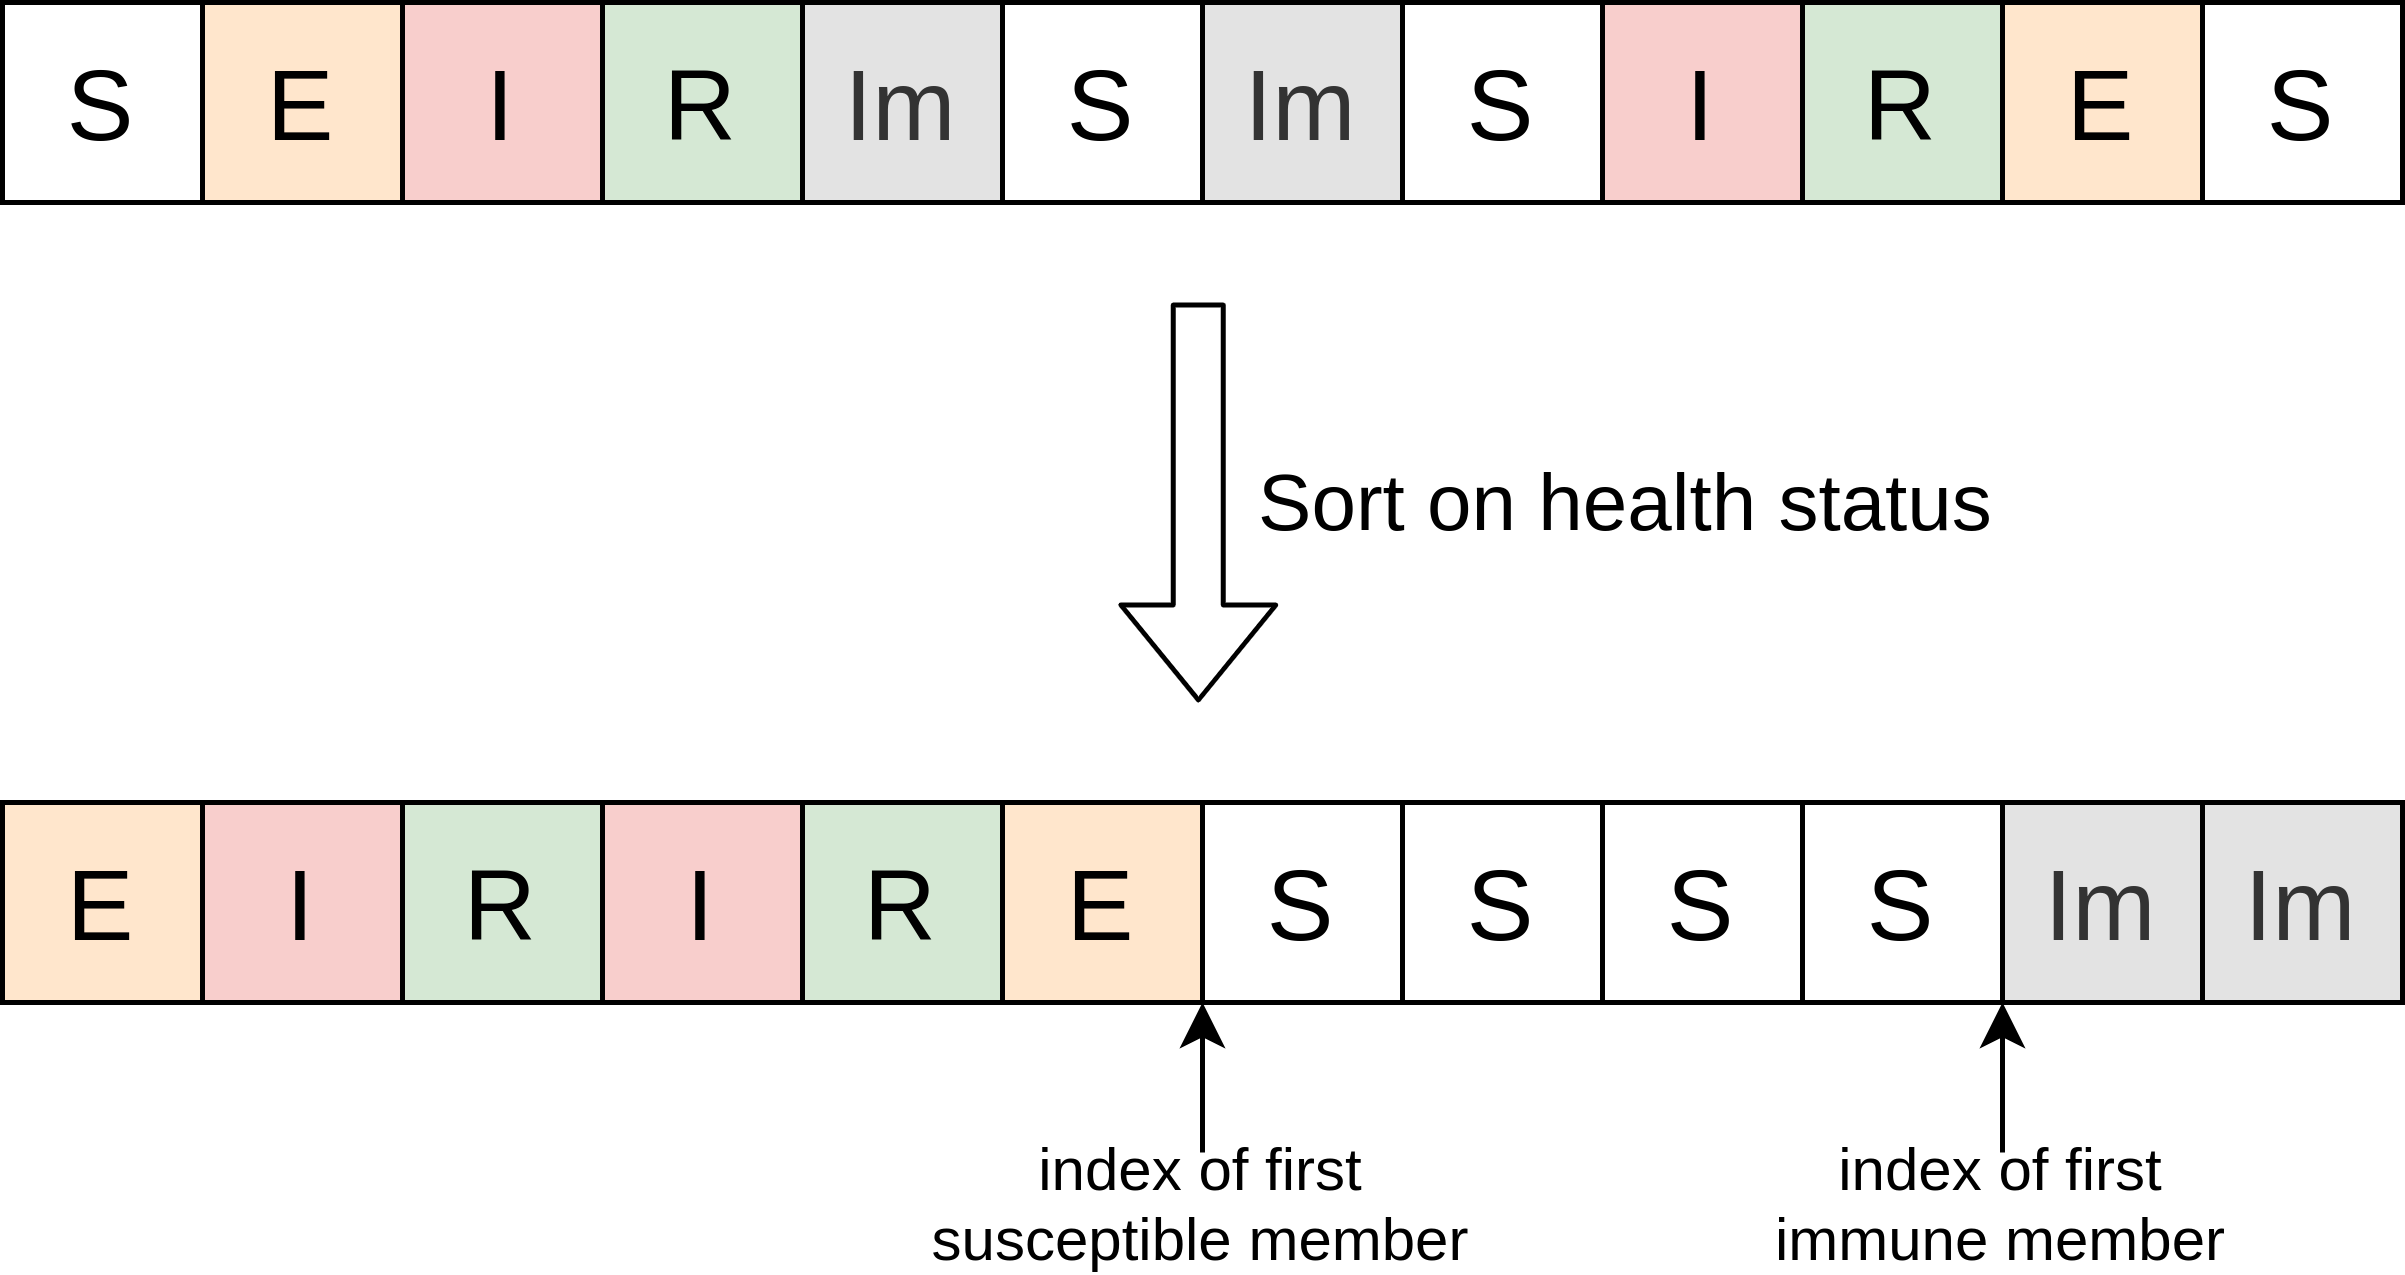
\includegraphics[width=.8\textwidth]{3 - Stride/fig/health_sort.png}
    \caption{Visual representation of a list of contact pool members before and after being sorted on health status, where every square represents a member. The letters indicate the health status of a member: Susceptible, Exposed, Infectious, Recovered, or Immune.}
    \label{fig:health_sort}
\end{figure}

\begin{algorithm}
\caption{Pseudo code of the function that sorts the members of a contact pool based on their health statuses.}
\label{alg:health_sorting}
\begin{algorithmic}[1]
    \Require{$P_{1} \dots P_{N}$, $i_{imm}$} \Comment{All members of the pool, index of first immune member}\;
    \Ensure{$P[\;] sorted$, $i_{imm}$, $i_{sus}$}
    \Statex
    \State $i_{sus} \gets 1$\Comment{Index of first susceptible member}
    \For{$i \gets 1$ to $i_{imm}$}\Comment{Iterate over the pool members}
        \State $member \gets P[i]$
        \If{member is immune}
            \State $i_{imm} \gets i_{imm}-1$
            \State $swapped \gets false$
            \While{$i_{imm} > i$ and not $swapped$}
                \State $member_{2} \gets P[i_{imm}]$
                \If{$member_{2}$ is immune}
                    \State $i_{imm} \gets i_{imm}-1$
                \Else
                    \State \Call{swap}{$member, member_{2}$}\Comment{Switch positions in $P[\;]$}
                    \State $swapped \gets true$
                \EndIf
            \EndWhile
        \Statex
        \ElsIf{member not susceptible}
            \If{$i_{sus} < i$}
                \State $member_{2} \gets P[i_{sus}]$
                \State \Call{swap}{$member, member_{2}$}\Comment{Switch positions in $P[\;]$}
            \EndIf
            \State $i_{sus} \gets i_{sus}+1$
        \EndIf
    \EndFor
    \State \Return $P[\;]$, $i_{imm}$, $i_{sus}$
\end{algorithmic}
\end{algorithm}

\subsubsection{Contact probability}
Calculating the probability that two people have contact with each other takes a lot of factors into account, so only an abstract explanation of this will be given here. The pseudo code of the function that does these calculations is given in Algorithm \ref{alg:contact_probability}. If the type of pool is a household, the contact probability is always $0.999$. Otherwise, the first step is to retrieve the contact rate for both individuals in the specific pool type, which is further explained in Section \ref{subsec:contact_matrix}. This number is a representation of how many contacts someone has in a specific pool type per day by looking at their age. These numbers are selected from the contact matrix, which is a configuration file, as seen in Section \ref{subsec:configurations}, based on the type of pool and the age of each individual. The lowest contact rate between the two individuals is then chosen as the definite number. This number is then multiplied by a contact adjustment factor based on the type of pool, which can be altered through the configurations. The adjustment factor is used, for example, to implement social distancing or intensify the contacts. The contact probability is then calculated by dividing these adjusted number of contacts by the total number of members in the pool minus one. This minus one represents a person themselves, with whom they of course cannot have contact with.

\begin{algorithm}
\caption{Pseudo code of the function that calculates the contact probability between two individuals in a contact pool.}
\label{alg:contact_probability}
\begin{algorithmic}[1]
    \Require{$P_{1}$,  $P_{2}$, $type$, and N}\Comment{Individuals, type of pool and total number of members}
    \Ensure{$prob$}\Comment{Probability of $P_{1}$ and $P_{2}$ having contact}
    \Statex
    \If{type = Household}
        \State \Return $0.999$
    \EndIf
    \Statex
    \State $contacts_{p1} \gets$ contact rate in pool($type$) for age($P_{1}$)
    \State $contacts_{p2} \gets$ contact rate in pool($type$) for age($P_{2}$)
    \State $contacts \gets min(contacts_{p1}, contacts_{p2})$
    \Statex
    \State  $factor \gets$ contact adjustment factor based on $type$
    \State $contacts \gets contacts * factor$
    \State $prob \gets contacts / (N-1)$
    \Statex
    \State $prob \gets min(prob, 0.999)$\Comment{Probability never higher than $0.999$}
    \State \Return $prob$
\end{algorithmic}
\end{algorithm}

\subsubsection{Transmission probability}
The probability of an infectious person transmitting their disease to a susceptible person when making contact depends on the combination of two things:
\begin{enumerate}
    \item The transmission probability of the disease itself, which is defined in the disease characteristics configurations.
    \item The relative transmission factor from the infected to the susceptible. This is based on a factor that represents the susceptibility if the susceptible person is younger than 18 years old, and the transmissibility if the infected is asymptomatic.
\end{enumerate}

\section{Data}
\label{sec:data}
Now that we have a better understanding of how our model works, we want to know what data it uses and how this data looks like. Because Stride can be run with different configurations and data, our goal here is not to focus on the data that has been used and examine it. Rather, we want to gain insight in the data that we will be using for the rest of this thesis, so that we can keep this knowledge in mind when analysing results. Eventually, our objective is to improve Stride in general, not just for a specific set of data.

\subsection{Population}
\label{subsec:population_data}
The first type of data we will look at is the population, for which Stride primarily uses the census data for Belgium from Eurostat\footnote{\url{https://ec.europa.eu/eurostat}}. For the research and tests of this thesis we used three different population representations, based on the 2011 census, which are also being used by the main researches of Stride: 600k, 3M, and 11M. These names are also an indication of the number of people every population contains, which is respectively 600 thousand, 3 million, and 11 million. 11M is the most accurate representation of the Belgian population and is naturally used for simulations regarding Belgium. 600k and 3M are smaller versions of the 11M which we only used when testing our optimisations. Therefore, we only discuss the 11M population in this section, of which the age distribution is shown in Figure \ref{fig:age_distribution}.

\begin{figure}
    \centering
    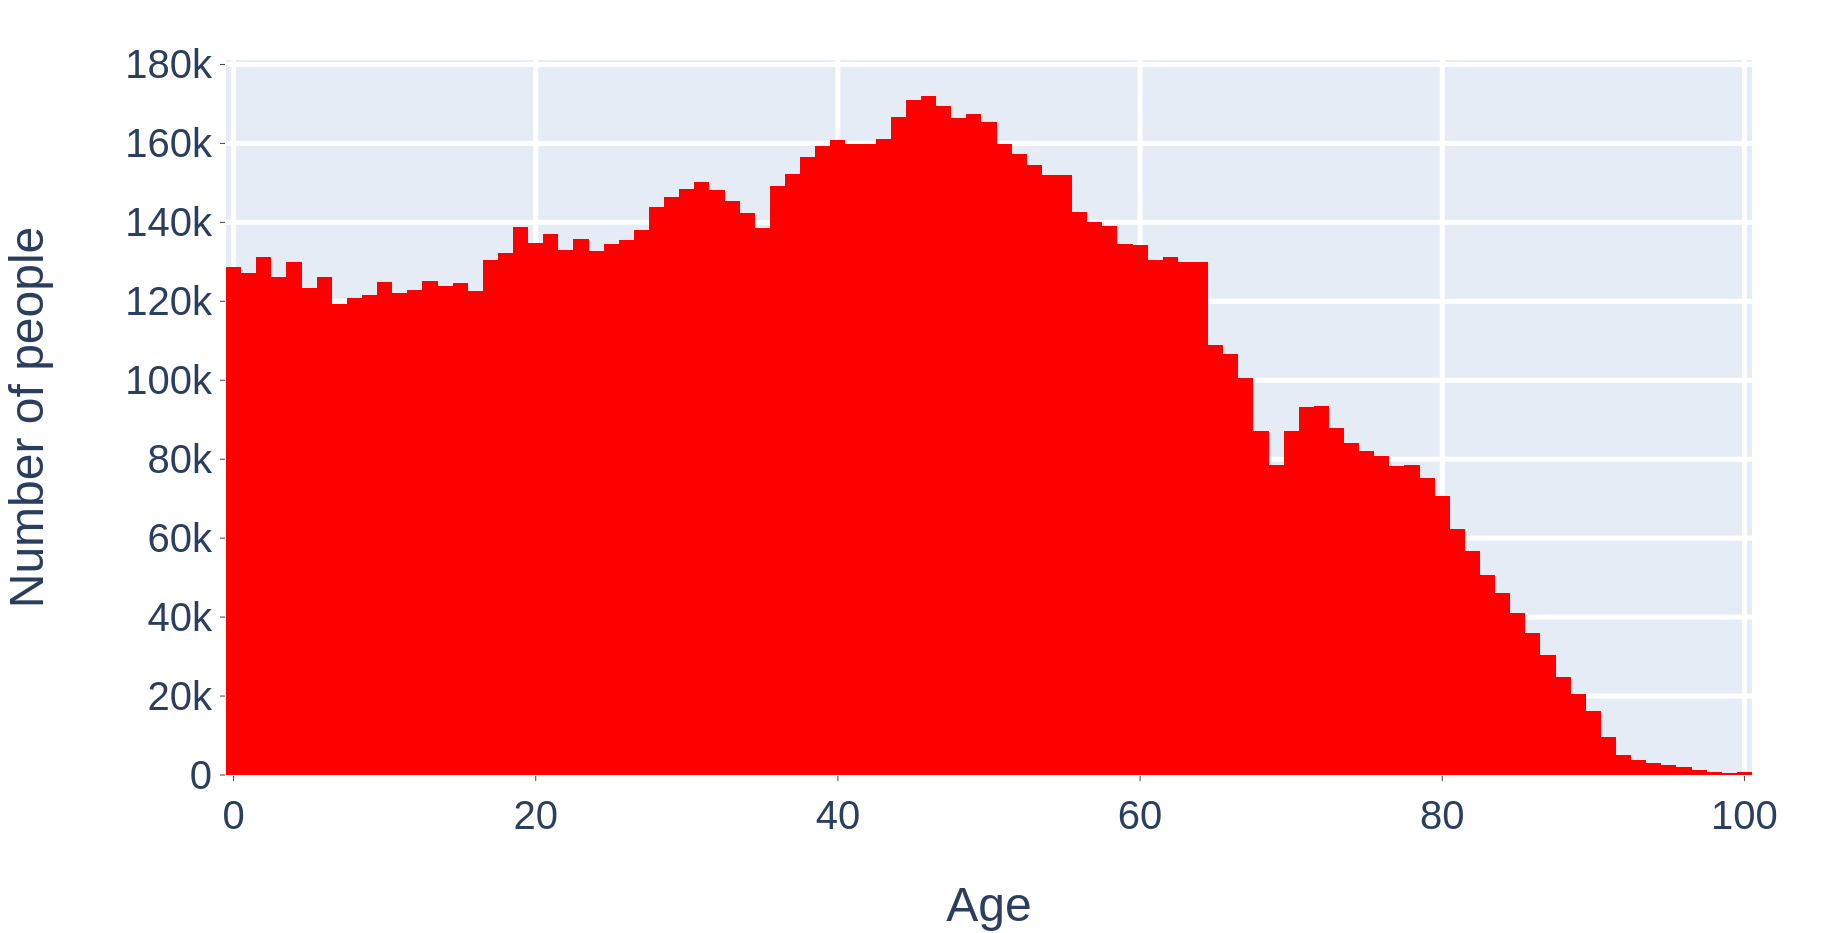
\includegraphics[width=.8\textwidth]{3 - Stride/fig/population_age_distribution.png}
    \caption{Age distribution of the 11M population.}
    \label{fig:age_distribution}
\end{figure}

\subsection{Contact pools}
\label{subsec:contact_pools_data}
All of the action in a Stride simulation occurs in the contact pools. This is where individuals have contact with one another and transmit the disease. Table \ref{tab:contact_pools_statistics} presents the general statistics of the different pool types next to each other. We see that there are vastly more household pools than any other type, but they are very small with a maximum of 6 and an average of 2.3 people per pool. The primary and secondary communities seem to be very similar and their average sizes are noticeably large. Workplaces can contain up to a thousand people, but are disproportionate compared to the other pool types with an average of 7.8 people. The school pools do not show any remarkable traits, but we will see that its general statistics are somewhat misleading. This information gives us a first view of the contact pools, however, a more profound analysis for every specific pool type is definitely needed.

\begin{table}
\centering
\resizebox{\textwidth}{!}{%
\begin{tabular}{@{}lrrrrr@{}}
\toprule
 &
  \multicolumn{1}{l}{Household} &
  \multicolumn{1}{l}{School} &
  \multicolumn{1}{l}{Workplace} &
  \multicolumn{1}{l}{\begin{tabular}[c]{@{}l@{}}Primary\\ community\end{tabular}} &
  \multicolumn{1}{l}{\begin{tabular}[c]{@{}l@{}}Secondary\\ community\end{tabular}} \\ \midrule
Number of pools & 4,859,837 & 131,756 & 566,759 & 22,000 & 22,000 \\
Min. pool size  & 1         & 6       & 1       & 51     & 44     \\
Max. pool size  & 6         & 50      & 1000    & 1431   & 1437   \\
Avg. pool size  & 2.3       & 20      & 7.8     & 500    & 500    \\ \bottomrule
\end{tabular}
}
\caption{General statistics of the contact pools of the 11M population.}
\label{tab:contact_pools_statistics}
\end{table}

\subsubsection{Household}
Since the total number of people in a household lies between one and six, there is probably not much variation possible amongst the household pools. Figure \ref{fig:household_poolsize_distribution}, which displays the distribution of household pool sizes, confirms this statement. 

\begin{figure}
    \centering
    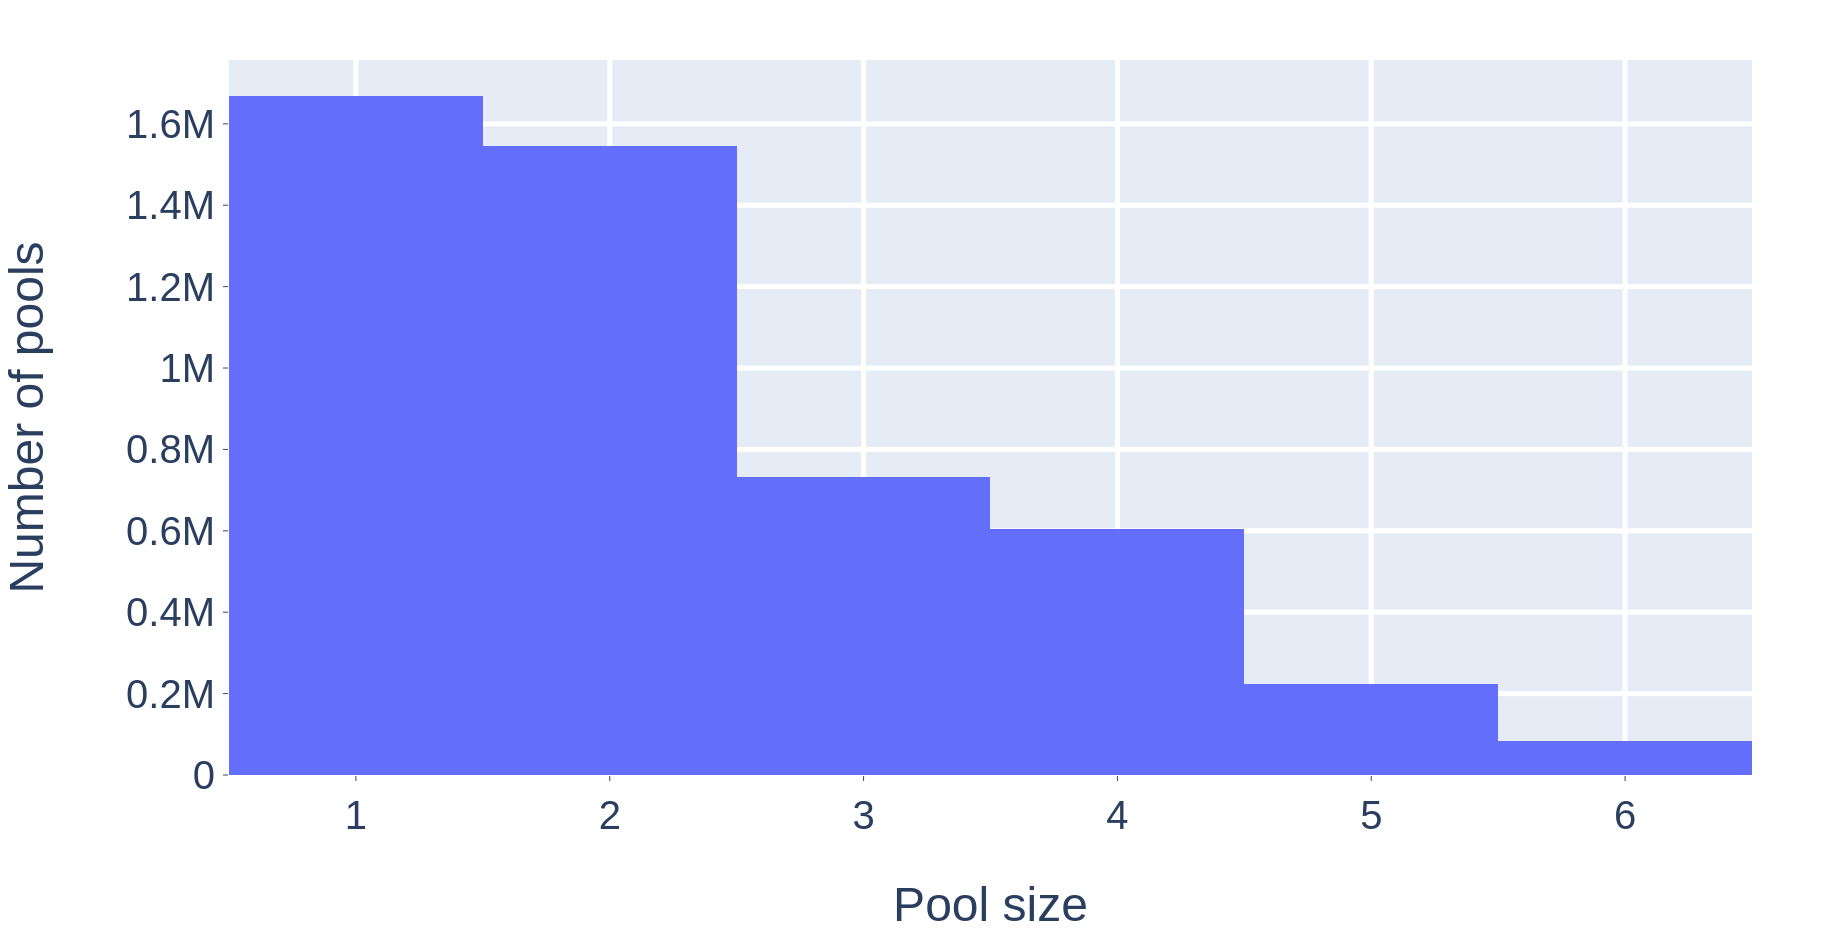
\includegraphics[width=.8\textwidth]{3 - Stride/fig/household_poolsizes.png}
    \caption{Distribution of the household pool sizes of the 11M population.}
    \label{fig:household_poolsize_distribution}
\end{figure}

\subsubsection{School}
Looking at the entire population, 24\% of the people have a school contact pool and only individuals younger than 60 years old can be a member, which Figure \ref{fig:school_age_distribution} shows us. In contrast with the general statistics, the distribution of school pool sizes in Figure \ref{fig:school_poolsize_distribution} shows that the school pool sizes are not evenly distributed and display a peculiar feature. We notice three different size `clusters': pools with size 1 to 10, 14 to 24, and 50. There is not much information that we can use from our 11M population to interpret these results, except for the age of the individuals in each cluster. Further inspection of the school contact pools with size 50 show that every individual is at least 18 years old. It is thus safe to assume that these only represent the college contact pools, which is also a logical explanation for the relative large pool sizes. The other two clusters do not show any age-specific traits, so we cannot say with certainty that these are only K-12 schools.

\begin{figure}
    \centering
    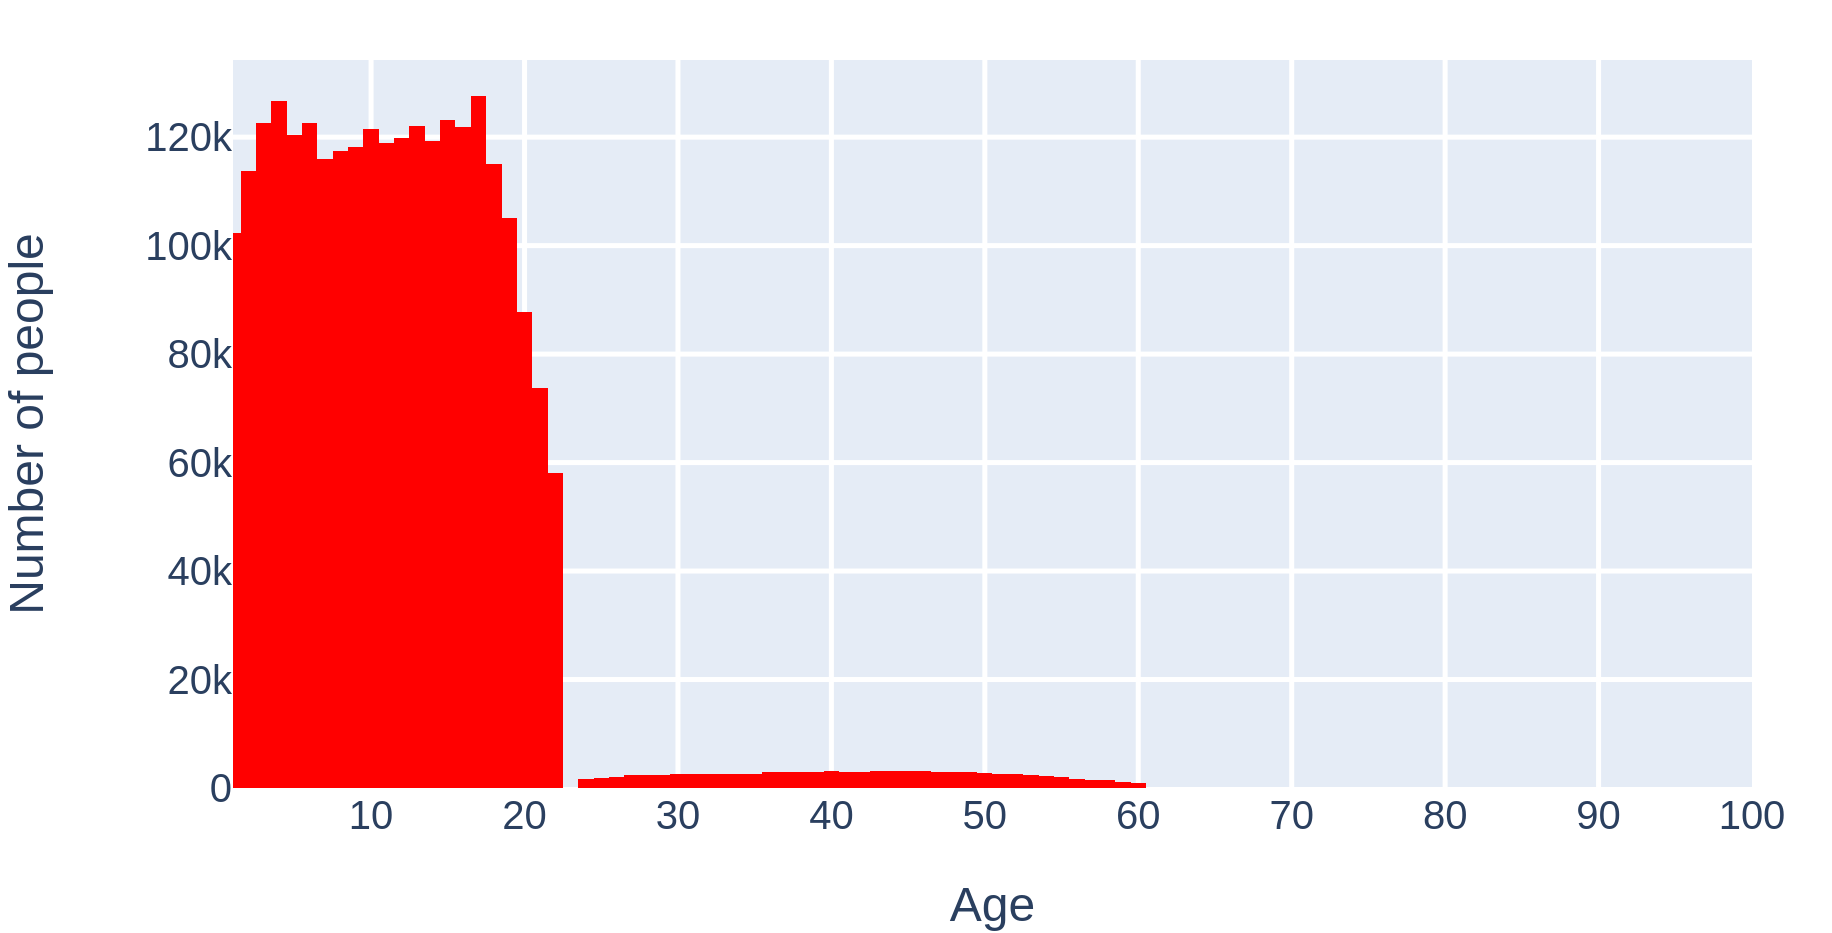
\includegraphics[width=.8\textwidth]{3 - Stride/fig/school_age_distribution.png}
    \caption{Age distribution of all the individuals that have a school contact pool in the 11M population.}
    \label{fig:school_age_distribution}
\end{figure}

\begin{figure}
    \centering
    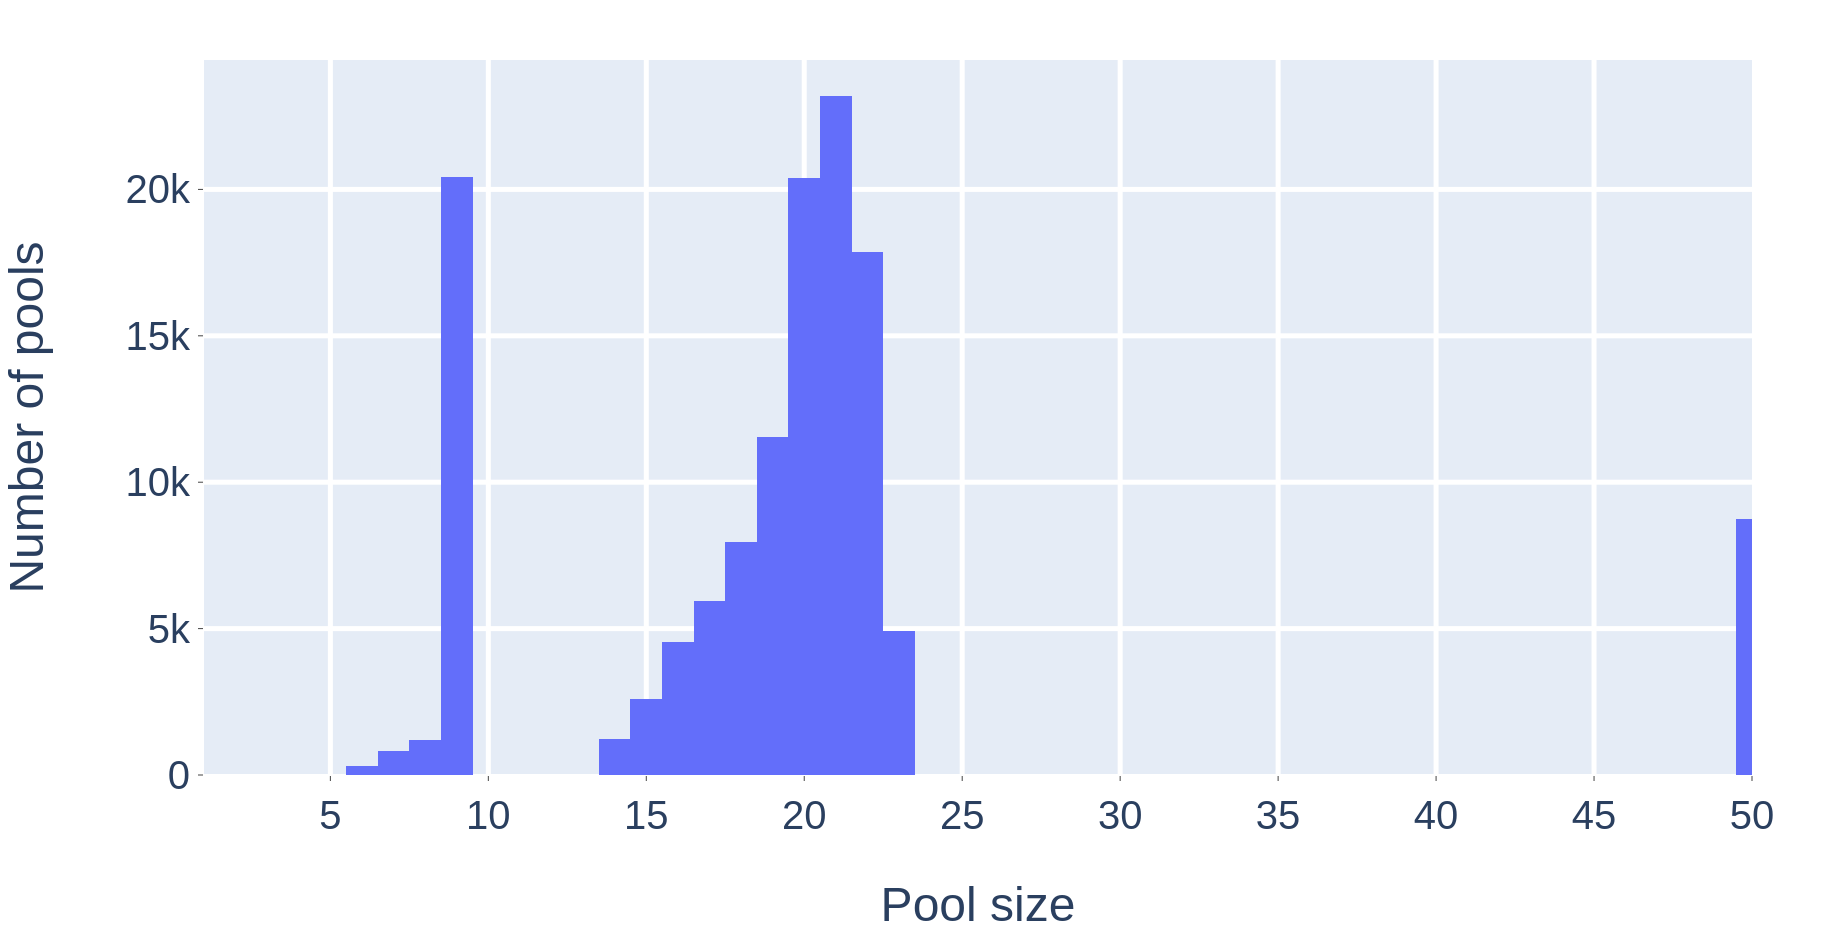
\includegraphics[width=.8\textwidth]{3 - Stride/fig/school_poolsizes.png}
    \caption{Distribution of the school pool sizes of the 11M population.}
    \label{fig:school_poolsize_distribution}
\end{figure}

\subsubsection{Workplace}
Just like with schools, not everyone has a workplace pool. 40\% of the population has a workplace contact pool and only people between the ages 17 to 77 can be a part of one, which is shown in Figure \ref{fig:workplace_age_distribution}. We also noticed how the workplace contact pools can contain one to a thousand people with an average size of 7.8. The distribution of workplace contact pool sizes displayed in Figure \ref{fig:workplace_all_poolsizes}, gives us insight into why this average size is so low. We clearly see that there is a major difference in the number of workplace pools with small sizes compared to the rest.
\\\\
In order to get a more detailed view of the number of workplace pools per size, we split them up in multiple age distribution ranges in Figure \ref{fig:workplace_poolsize_ranges}. The different ranges that we have chosen display more precisely the number of pools per pool size. We only notice that in Figure \ref{fig:workplace_10-50_poolsizes} there still is a big difference between the sizes smaller than 20 and the rest. Following this, we now look for `clusters' of pool sizes, or pool size ranges, in which the pool sizes in the same range have approximately the same number of pools. The ranges that we assume, looking at Figure \ref{fig:workplace_poolsize_ranges}, are: [1,9], [10,19], [20,49], [50,249], and [250,1000]. The statistics for these ranges in Table \ref{tab:workplace_stats}, confirm that our ranges contain pool sizes with similar number of pools. The range [1,9] contains, as expected, 94\% of all the workplace pools, but only consists of 60.5\% of the working individuals. So, although there are not that many workplace contact pools with more than nine people, they still account for 39.5\% of all the individuals with a workplace pool.

\begin{figure}
    \centering
    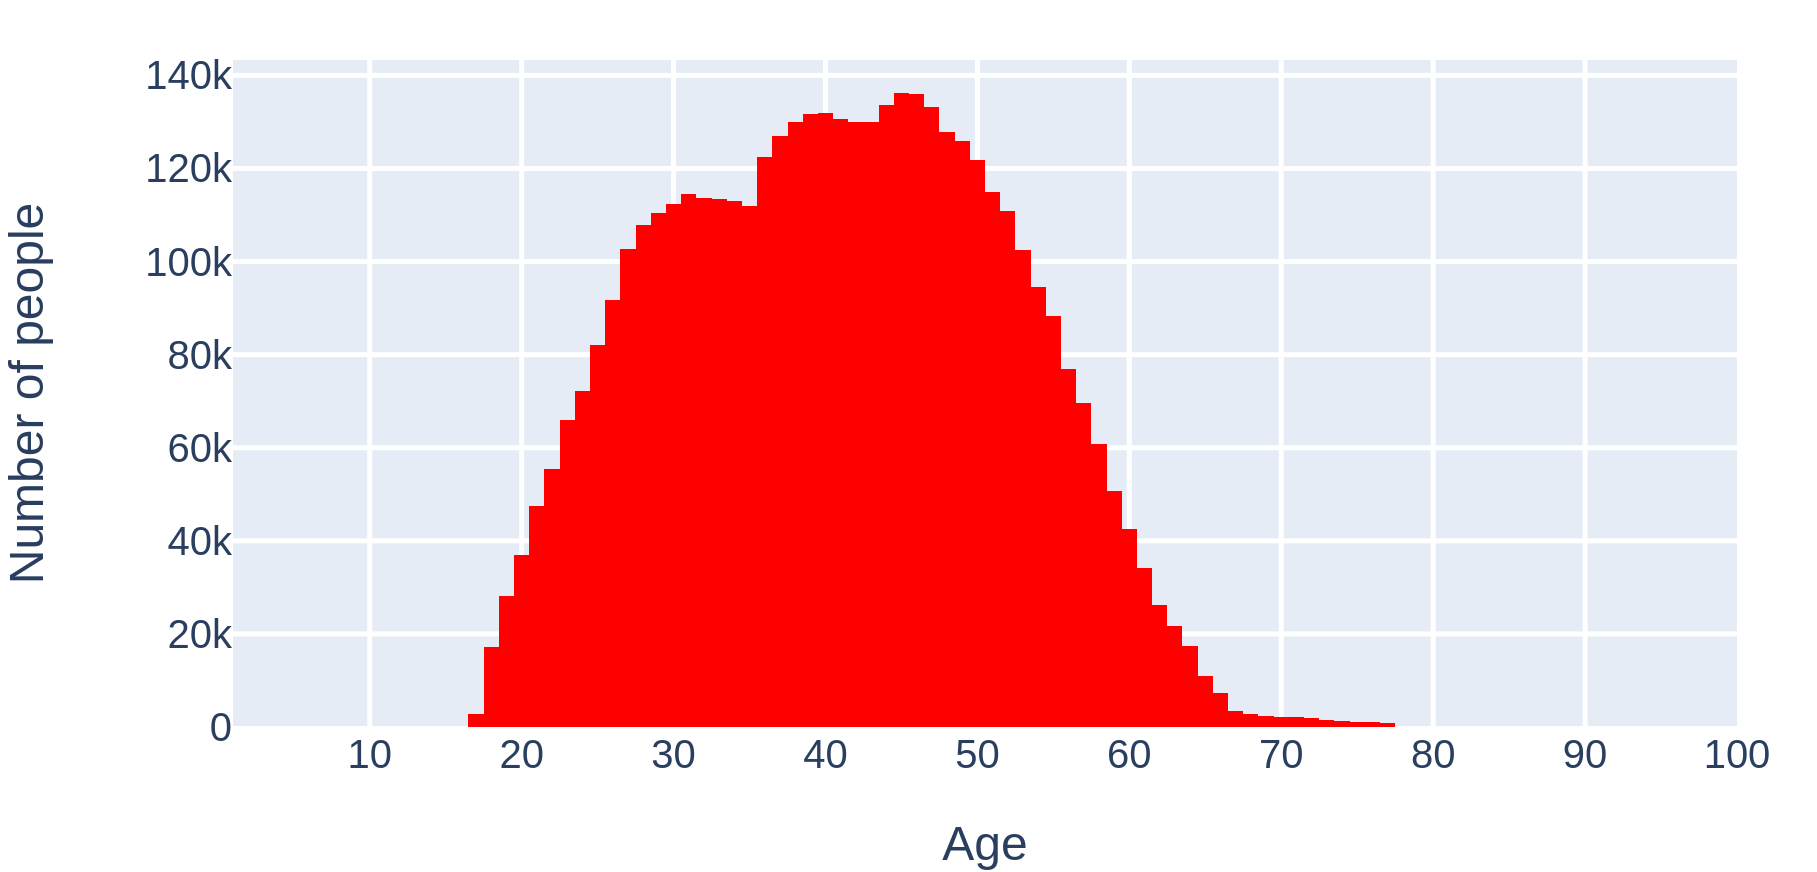
\includegraphics[width=.8\textwidth]{3 - Stride/fig/workplace_age_distribution.png}
    \caption{Age distribution of all the individuals that have a workplace contact pool in the 11M population.}
    \label{fig:workplace_age_distribution}
\end{figure}

\begin{figure}
    \centering
    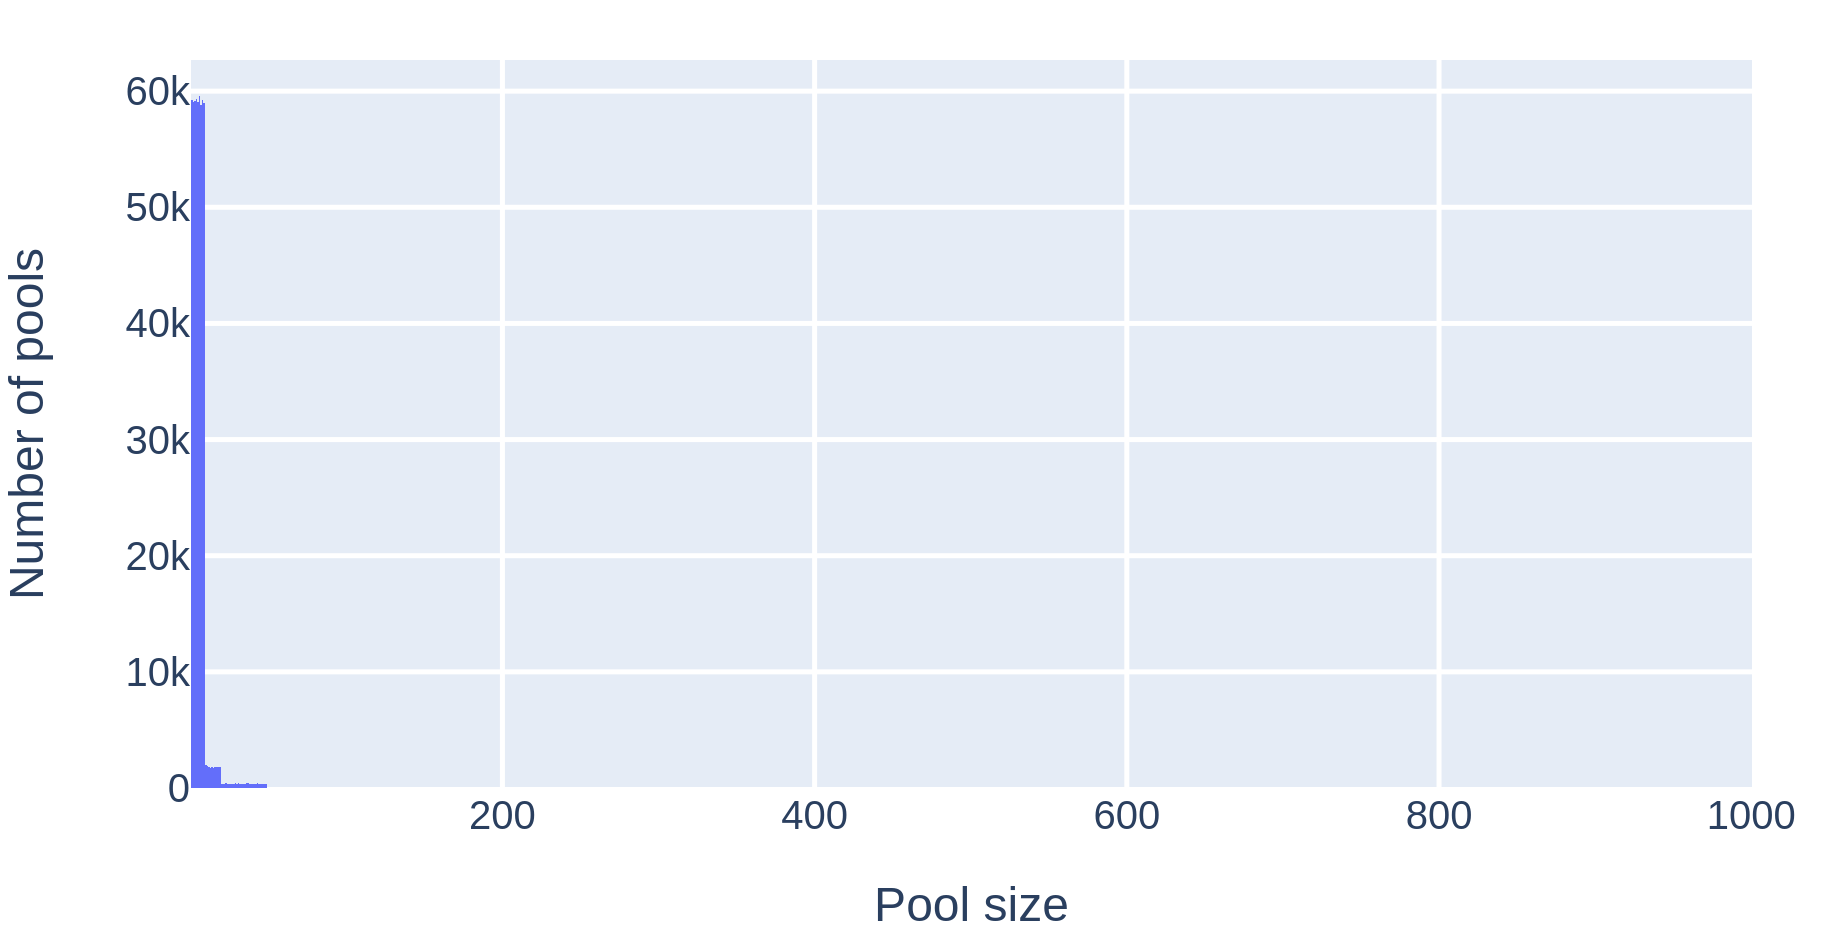
\includegraphics[width=.8\textwidth]{3 - Stride/fig/workplace_all_poolsizes.png}
    \caption{Distribution of the workplace pool sizes in the 11M population.}
    \label{fig:workplace_all_poolsizes}
\end{figure}

\begin{figure} 
  \begin{subfigure}[b]{0.5\linewidth}
    \centering
    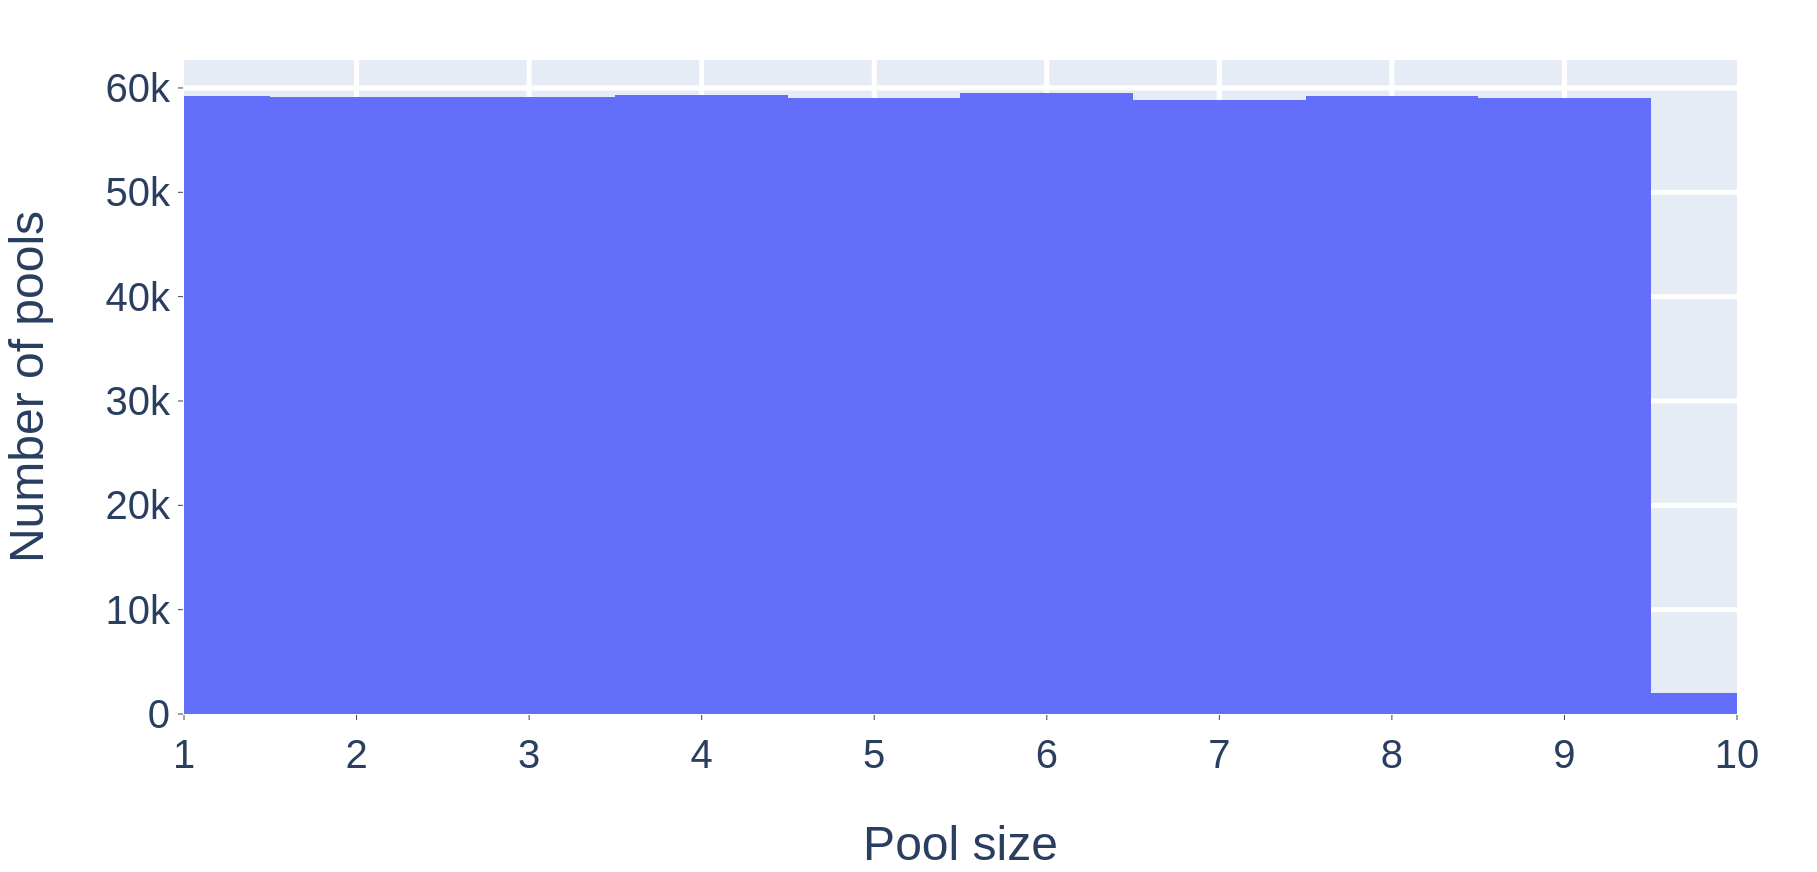
\includegraphics[width=\linewidth]{3 - Stride/fig/workplace_1-10_poolsizes.png} 
    \caption{Pool sizes 1 to 10.} 
    \label{fig:workplace_1-10_poolsizes} 
    \vspace{4ex}
  \end{subfigure}%% 
  \begin{subfigure}[b]{0.5\linewidth}
    \centering
    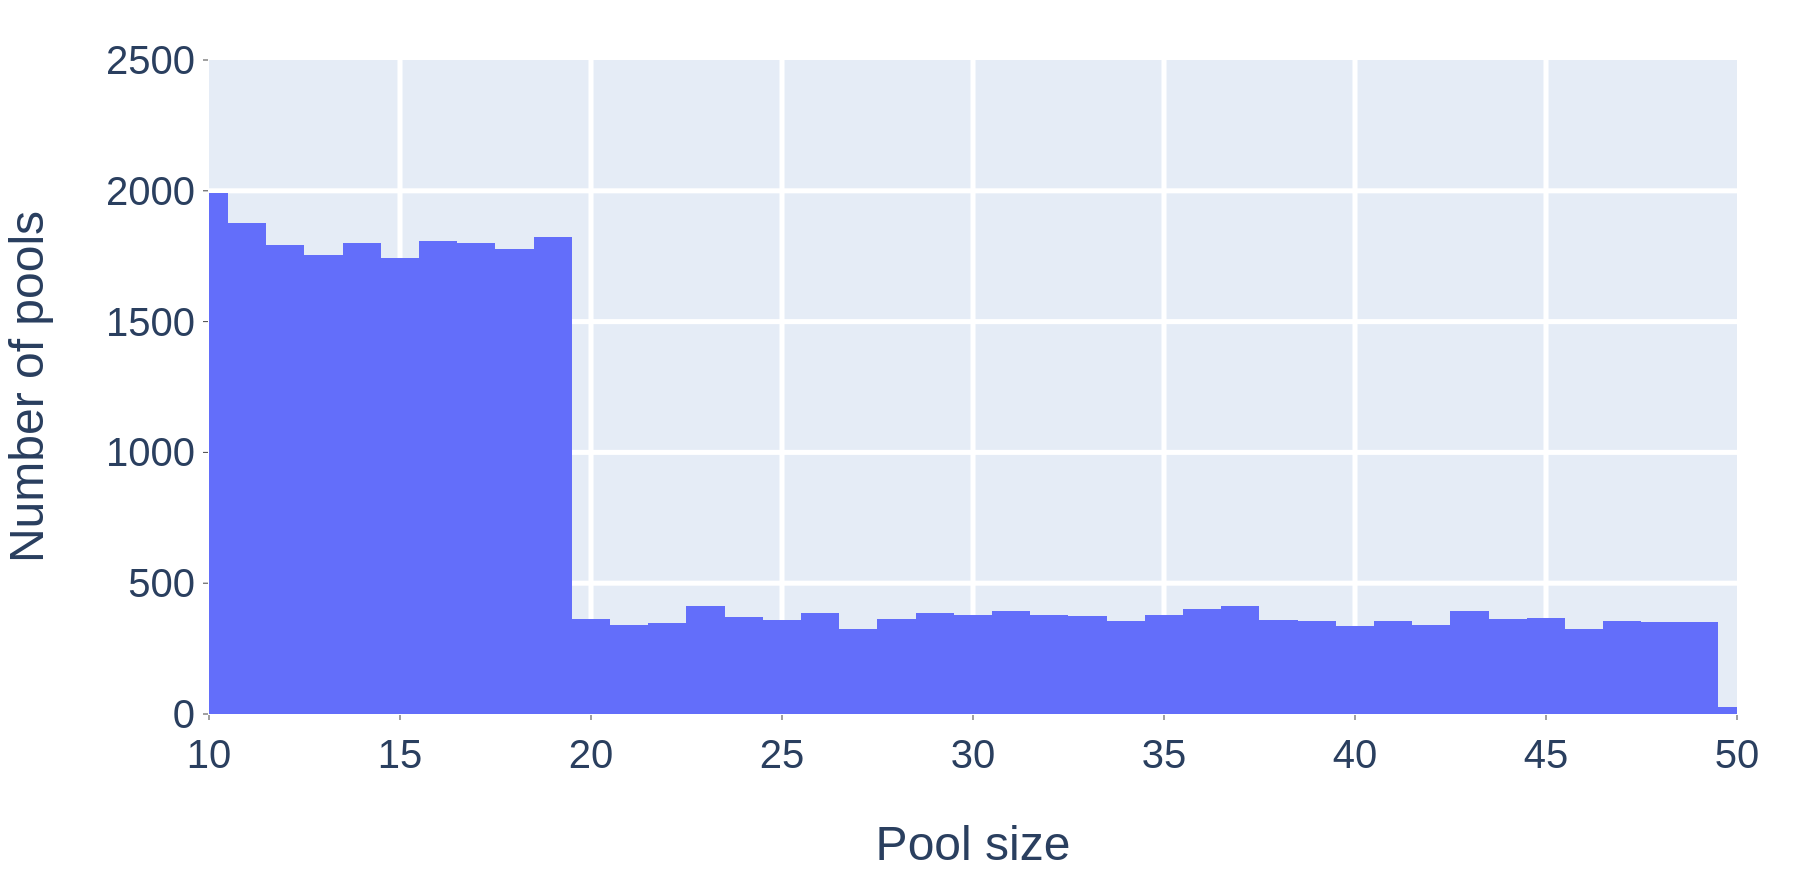
\includegraphics[width=\linewidth]{3 - Stride/fig/workplace_10-50_poolsizes.png} 
    \caption{Pool sizes 10 to 50.} 
    \label{fig:workplace_10-50_poolsizes} 
    \vspace{4ex}
  \end{subfigure} 
  \begin{subfigure}[b]{0.5\linewidth}
    \centering
    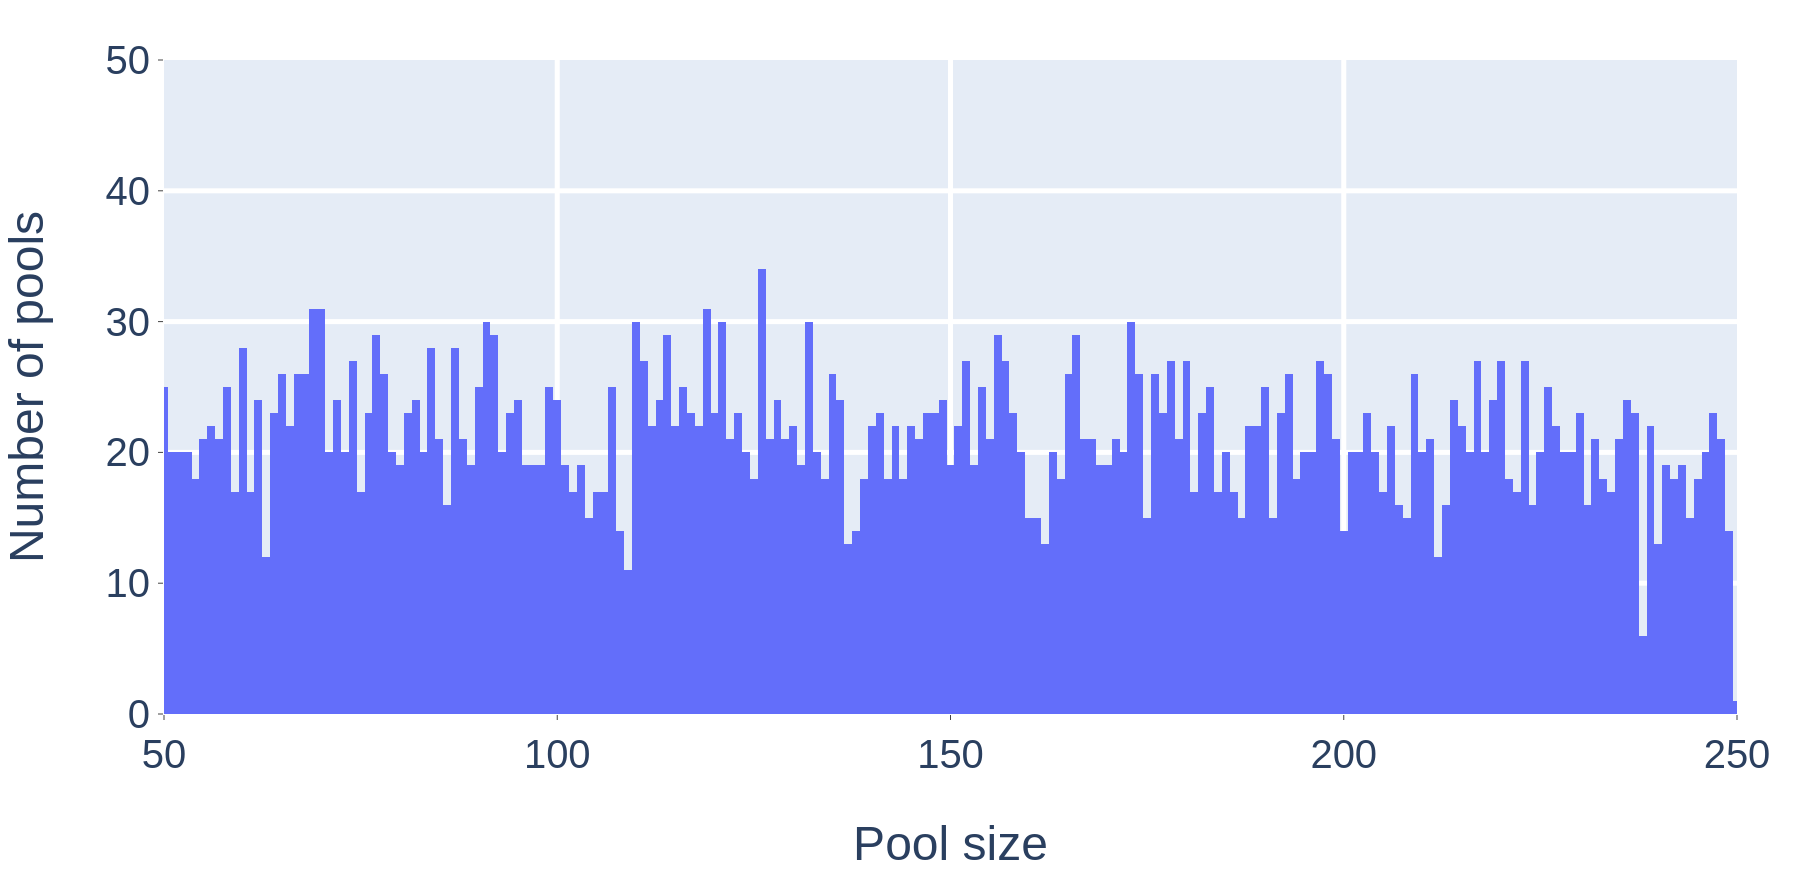
\includegraphics[width=\linewidth]{3 - Stride/fig/workplace_50-250_poolsizes.png} 
    \caption{Pool sizes 50 to 250.} 
    \label{fig:workplace_5-250_poolsizes} 
  \end{subfigure}%%
  \begin{subfigure}[b]{0.5\linewidth}
    \centering
    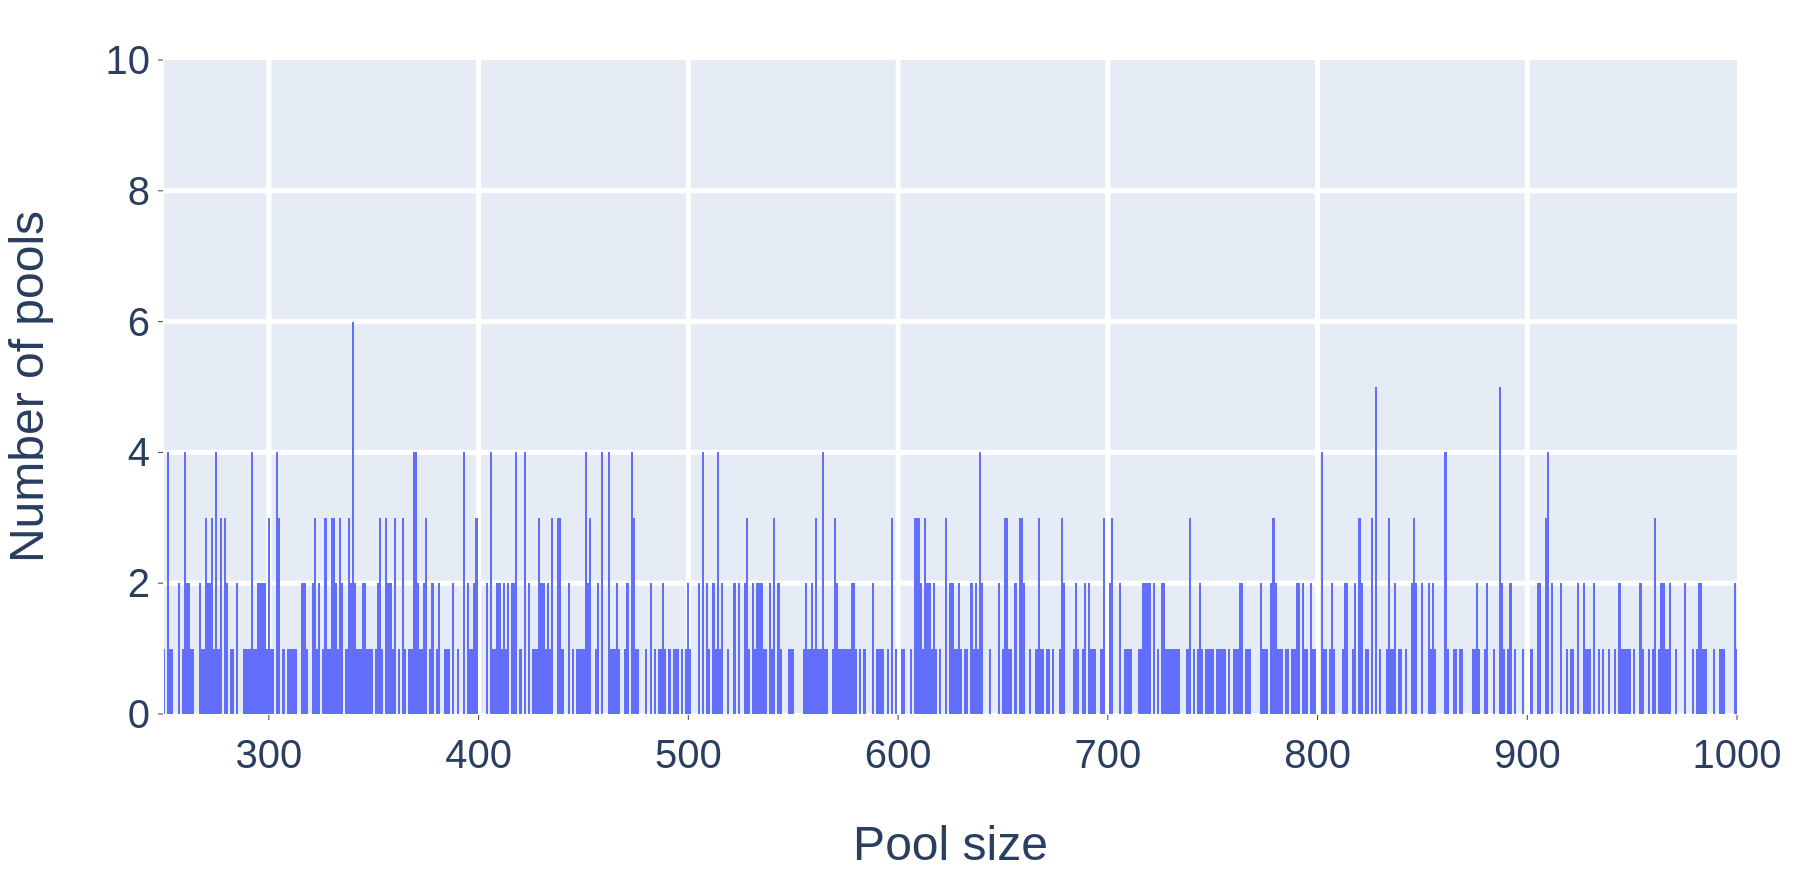
\includegraphics[width=\linewidth]{3 - Stride/fig/workplace_250-1000_poolsizes.png} 
    \caption{Pool sizes 250 to 1000.} 
    \label{fig:workplace_250-1000_poolsizes} 
  \end{subfigure} 
  \caption{Distributions of the workplace pool sizes from Figure \ref{fig:workplace_all_poolsizes} for different pool size ranges.}
  \label{fig:workplace_poolsize_ranges} 
\end{figure}

\begin{table}
\centering
\resizebox{\textwidth}{!}{%
\begin{tabular}{@{}lrrrrr@{}}
\toprule
Pool size range      & 1 - 9     & 10 - 19 & 20 - 49 & 50 - 249 & 250 - 1000 \\ \midrule
\begin{tabular}[t]{@{}l@{}}Minimum number of pools\\ (for a pool size)\end{tabular} &
  58,827 &
  1,744 &
  324 &
  \begin{tabular}[t]{@{}r@{}}6\\(11 excl. size 238)\end{tabular} &
  1 \\
\begin{tabular}[t]{@{}l@{}}Maximum number of pools\\ (for a pool size)\end{tabular} &
  59,547 &
  1,992 &
  414 &
  34 &
  6 \\ \midrule
Number of pools      & 532,518   & 18,169  & 10,983  & 4,286    & 803        \\
\% of pools          & 94.0      & 3.2     & 1.9     & 0.8      & 0.1        \\ \midrule
Number of people     & 2,661,724 & 262,427 & 377,612 & 629,345  & 467,110    \\
\% of working people & 60.5      & 6.0     & 8.6     & 14.3     & 10.6       \\ \bottomrule
\end{tabular}%
}
\caption{Statistics for the different workplace pool size ranges. The pool sizes in every size range have approximately the same amount of pools.}
\label{tab:workplace_stats}
\end{table}

\subsubsection{Primary \& secondary community}
When we looked at the general statistics of the community pool types, we noticed that the primary and secondary community contact pools had very similar results. Figures \ref{fig:primary_community_poolsizes} and \ref{fig:secondary_cumminity_poolsizes} demonstrate that these types of pools are nearly identical and both have a normal pool size distribution with a peak around size 500.

\begin{figure}
    \centering
    \begin{minipage}[b]{0.48\textwidth}
        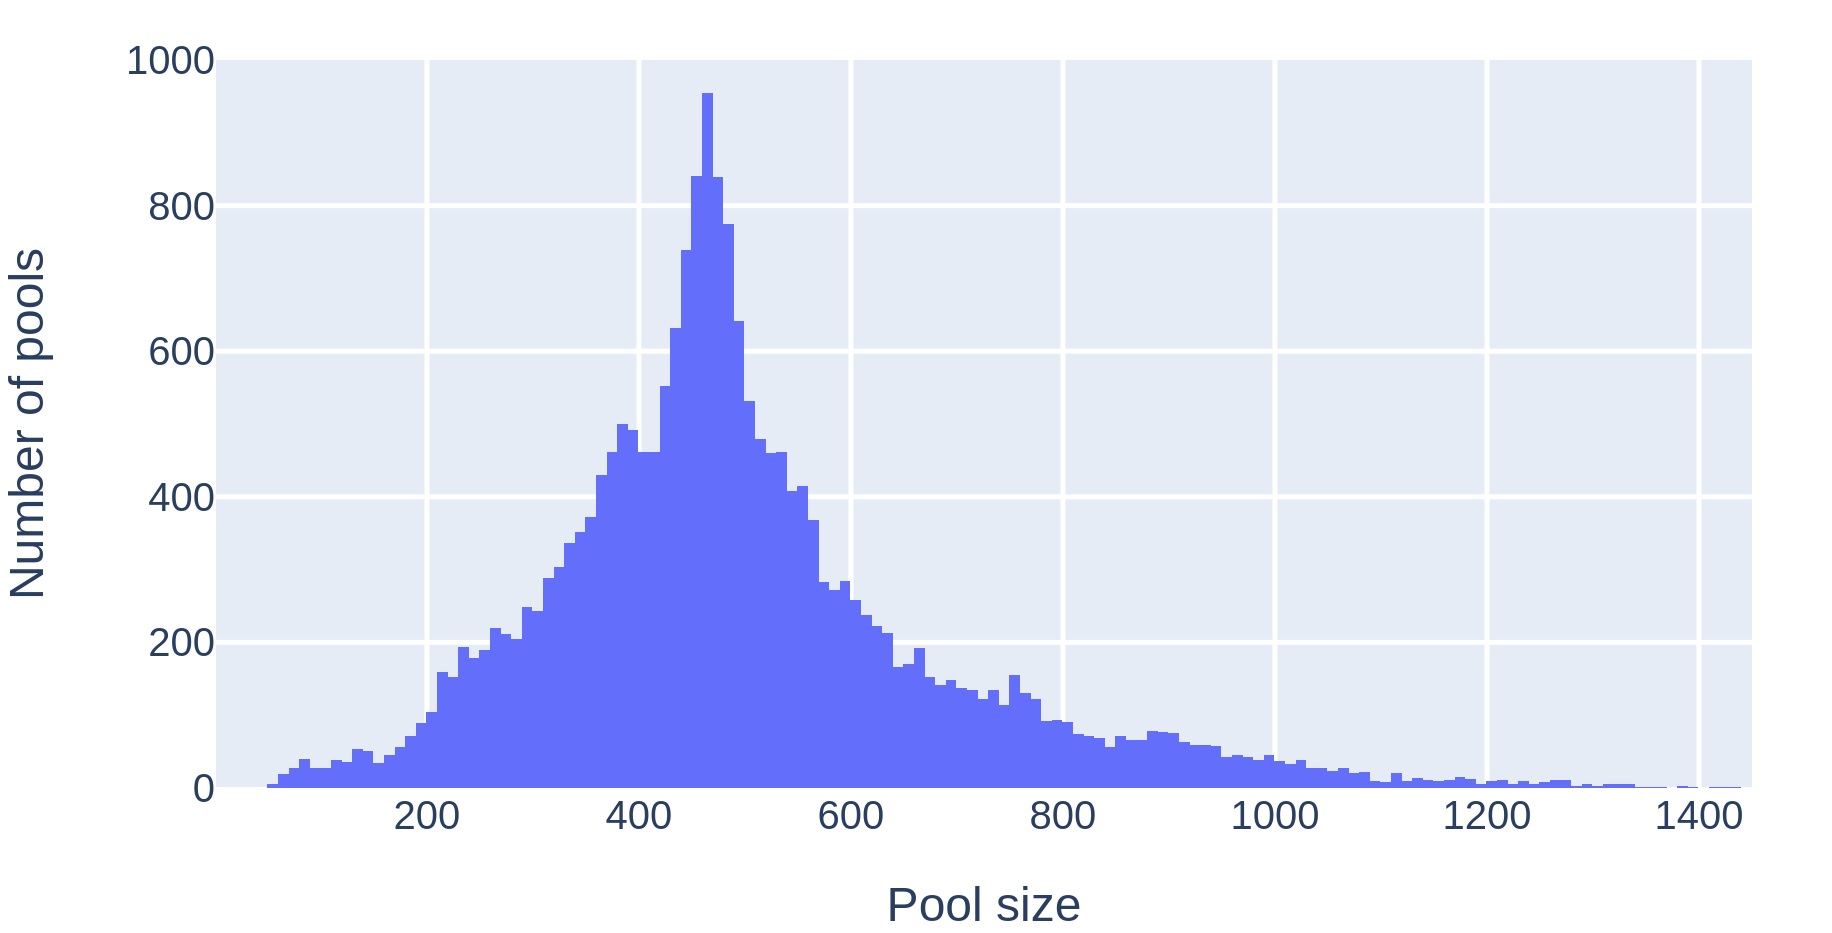
\includegraphics[width=\textwidth]{3 - Stride/fig/primary_community_poolsizes.png}
        \caption{Distribution of the primary community pool sizes of the 11M population.}
        \label{fig:primary_community_poolsizes}
    \end{minipage}
    \hfill
    \begin{minipage}[b]{0.48\textwidth}
        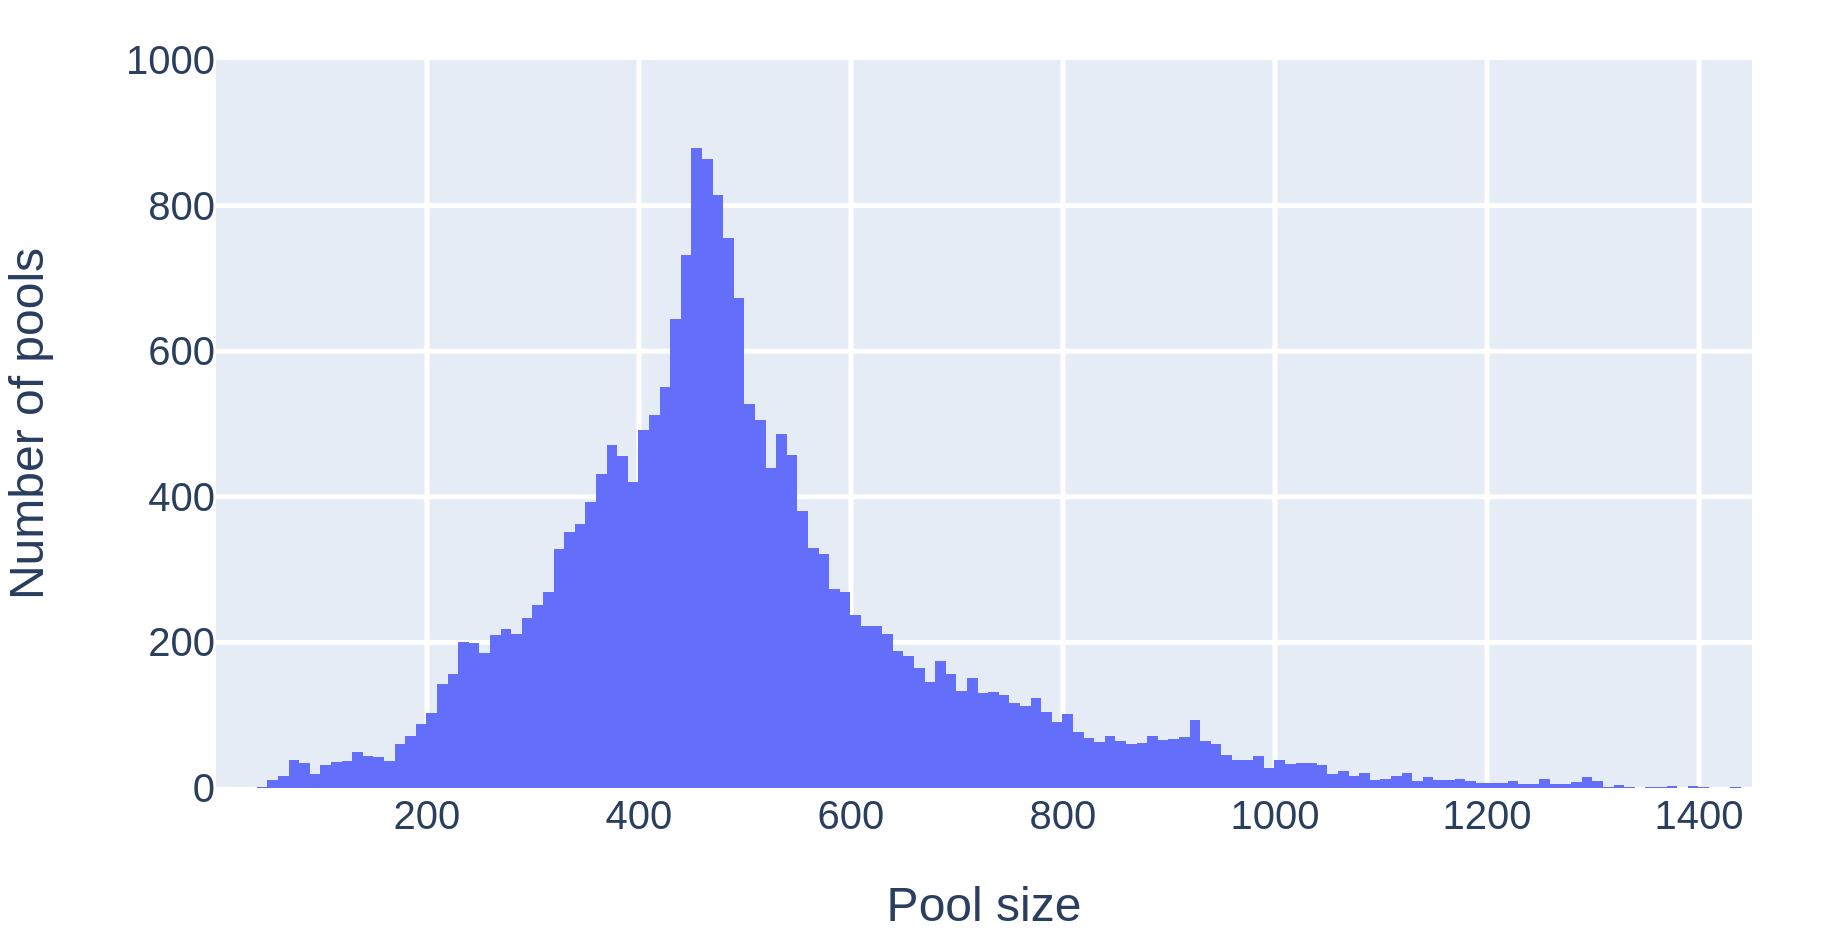
\includegraphics[width=\textwidth]{3 - Stride/fig/secondary_community_poolsizes.png}
        \caption{Distribution of the secondary community pool sizes of the 11M population.}
        \label{fig:secondary_cumminity_poolsizes}
    \end{minipage}
\end{figure}

\subsection{Contact matrix}
\label{subsec:contact_matrix}
In Section \ref{subsec:contacts_and_transmissions} we learned how Stride calculates a contact probability based on the configurated contact matrices, which was explained in Section \ref{subsec:configurations}. For every type of contact pool there exists a matrix which contains the contact rate based on age. The matrices for a school, workplace, primary community, and secondary community are respectively displayed in Figures \ref{fig:school_contact_rates}, \ref{fig:work_contact_rates}, \ref{fig:primary_contact_rates}, and \ref{fig:secondary_contact_rates}. These rates indicate the average number of contacts an individual has in a particular contact pool with respect to their own age. Algorithm \ref{alg:contact_probability} shows how the contact probability gets calculated between two individuals. The probability of two people having contact in a household is always $0.999$, therefore, we do not need a contact matrix for the household contact pool type.
\\\\
The data for these contact rates originates from SOCRATES, which is an online interactive tool\footnote{\url{http://www.socialcontactdata.org/socrates/}}, created by Willem et al. \cite{socrates}, for the sharing of social contact data. The data they present are 2D matrices in which the contact rate in a pool is based on the ages of the person who initiates contact and the one who receives it. These matrices for our contact pool types are visualised in Figure \ref{fig:contact_heatmaps}, which are different than the ones we presented. The contact rates that Stride uses are actually 1D matrices or just \textit{vectors}, which are based on those 2D matrices. These matrices have been transformed into our vectors so that contact rate look-ups are faster and easier to use. If we would use the actual matrices, with dimensions 112x112, the look-ups would take substantially more time than with our vectors. Thus, from now on we will refer to these 1D matrices as the \textit{contact vectors}. Furthermore, in the 2D matrices we again clearly see that people have the most contact with people who are the same age, with an exception in the workplace. This exception has an intuitive explanation, which is that people at work have contact with everyone disregarding age and that people at work are mostly between the ages of 18 to 65 years old. 

\begin{figure}
    \centering
    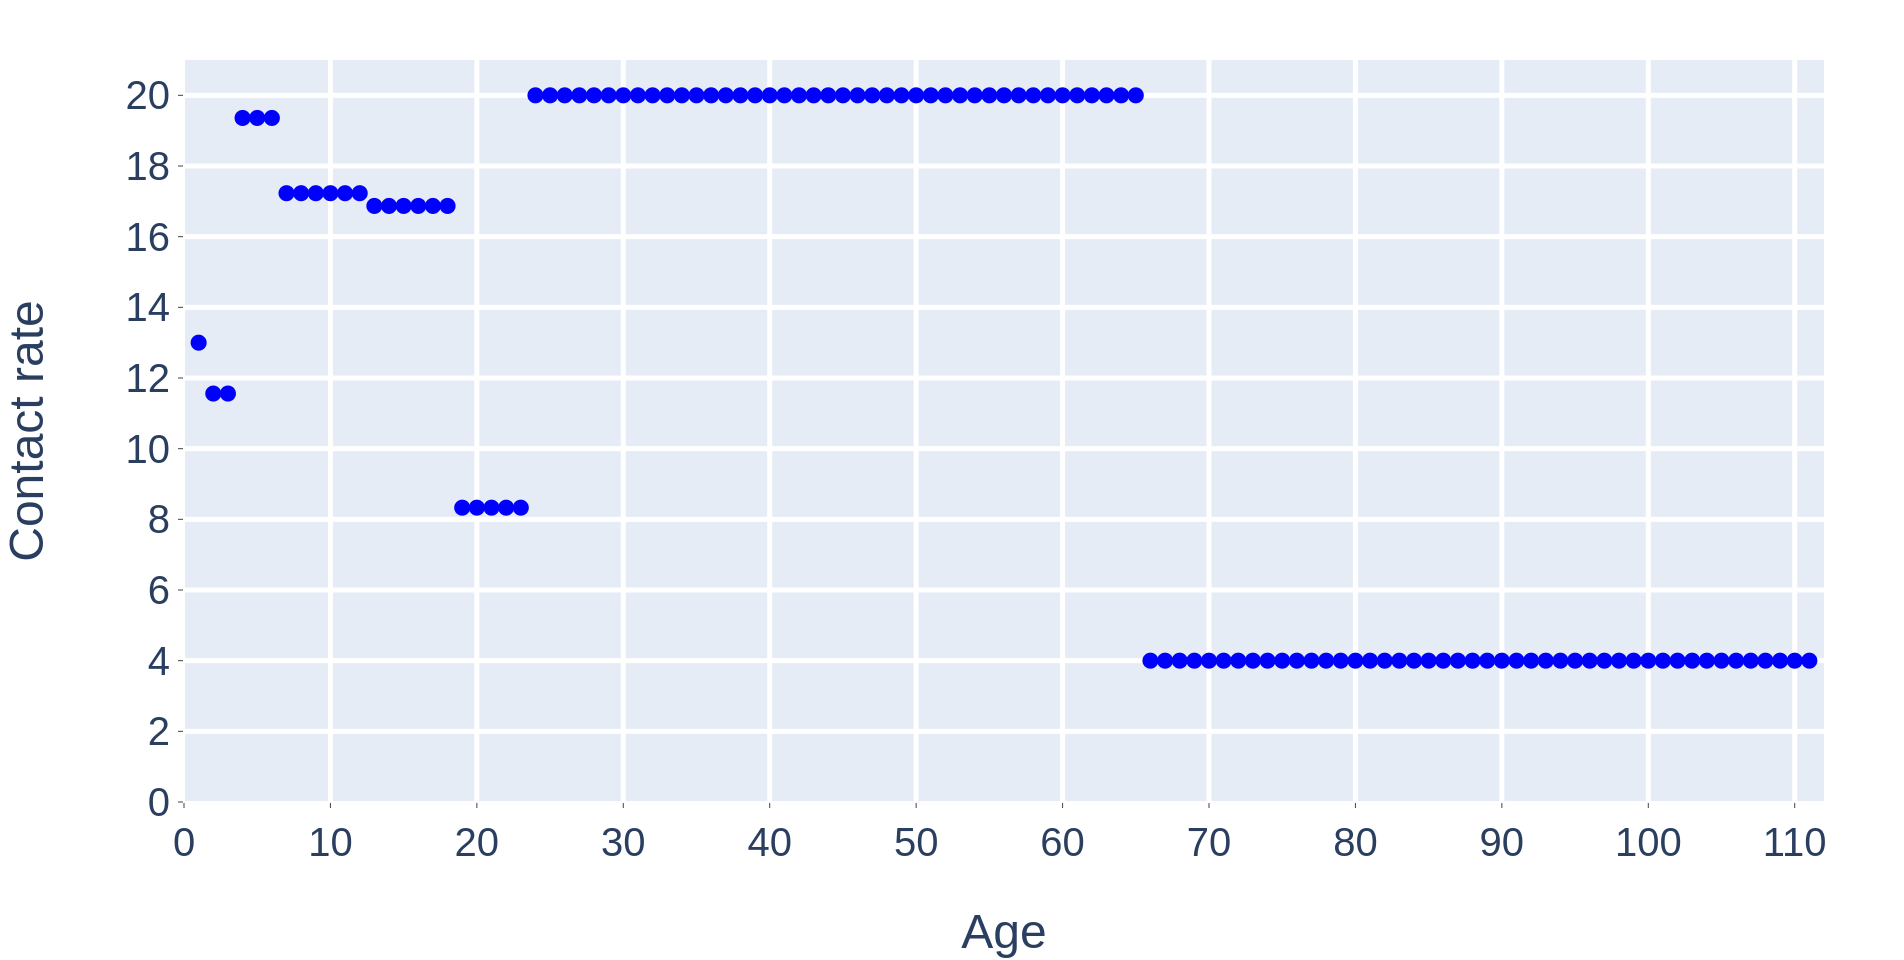
\includegraphics[width=.8\textwidth]{3 - Stride/fig/school_contact_rates.png}
    \caption{Contact rates per age at school.}
    \label{fig:school_contact_rates}
\end{figure}

\begin{figure}
    \centering
    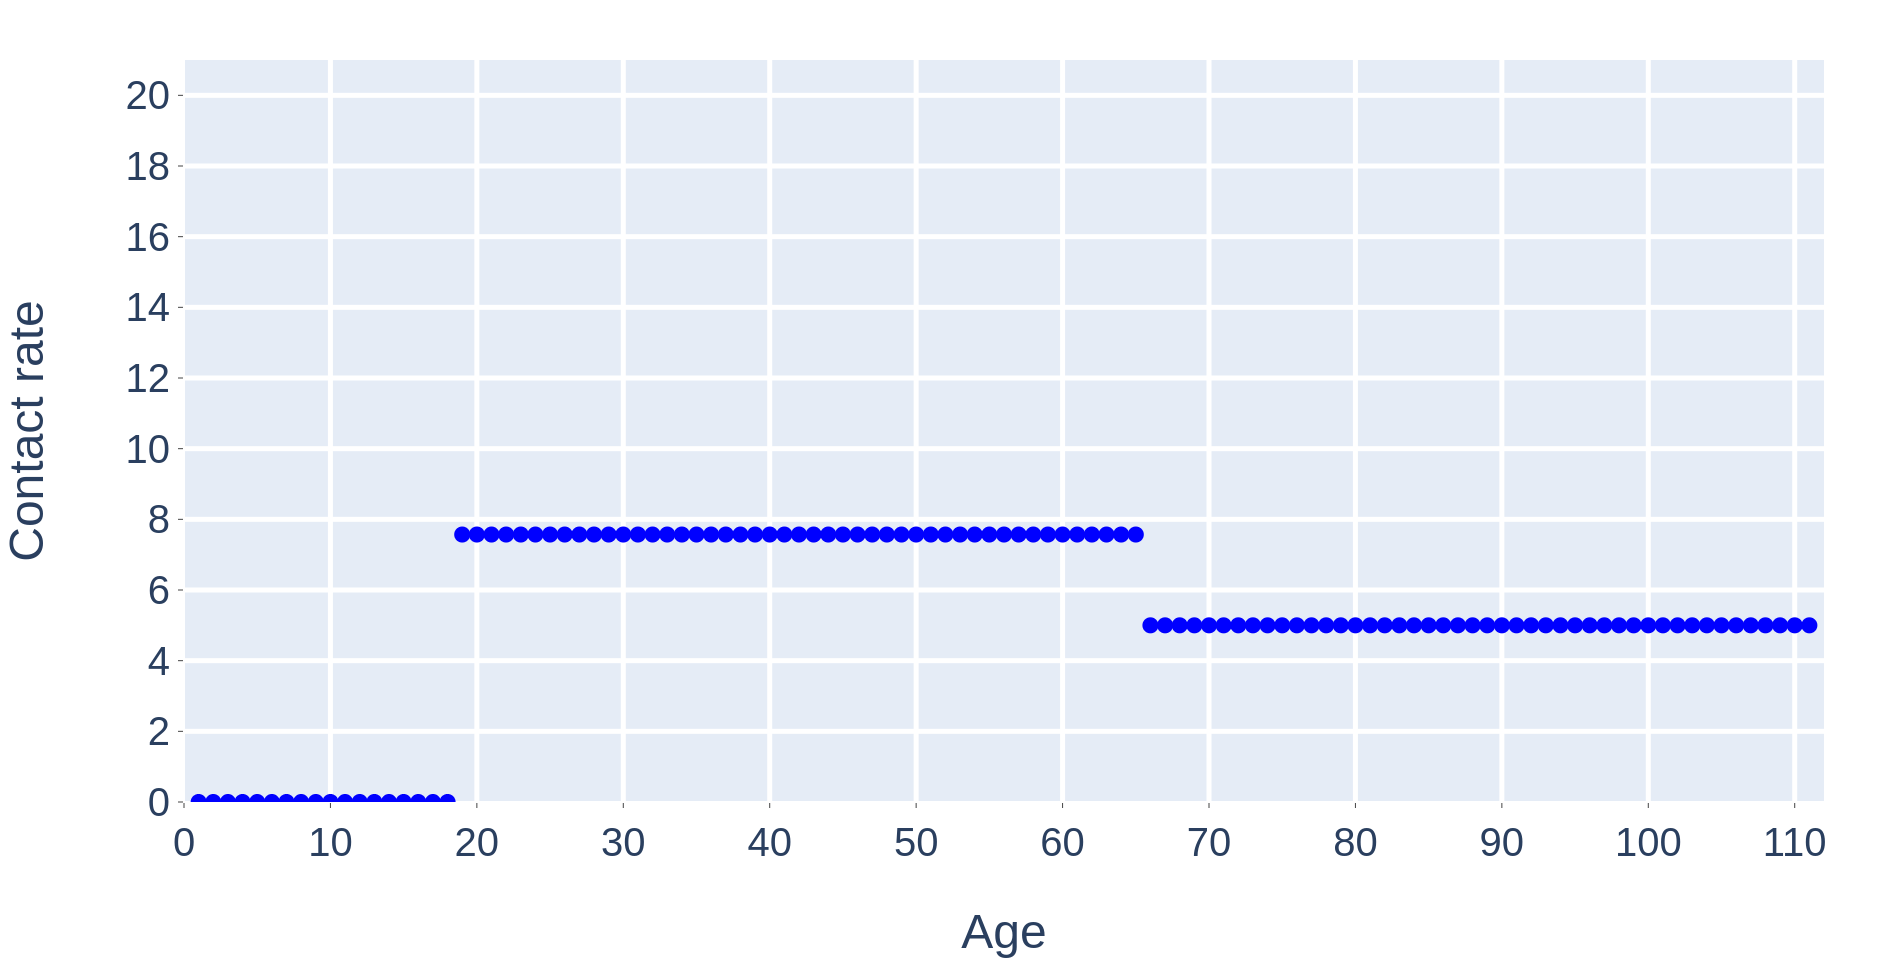
\includegraphics[width=.8\textwidth]{3 - Stride/fig/work_contact_rates.png}
    \caption{Contact rates per age at work.}
    \label{fig:work_contact_rates}
\end{figure}

\begin{figure}
    \centering
    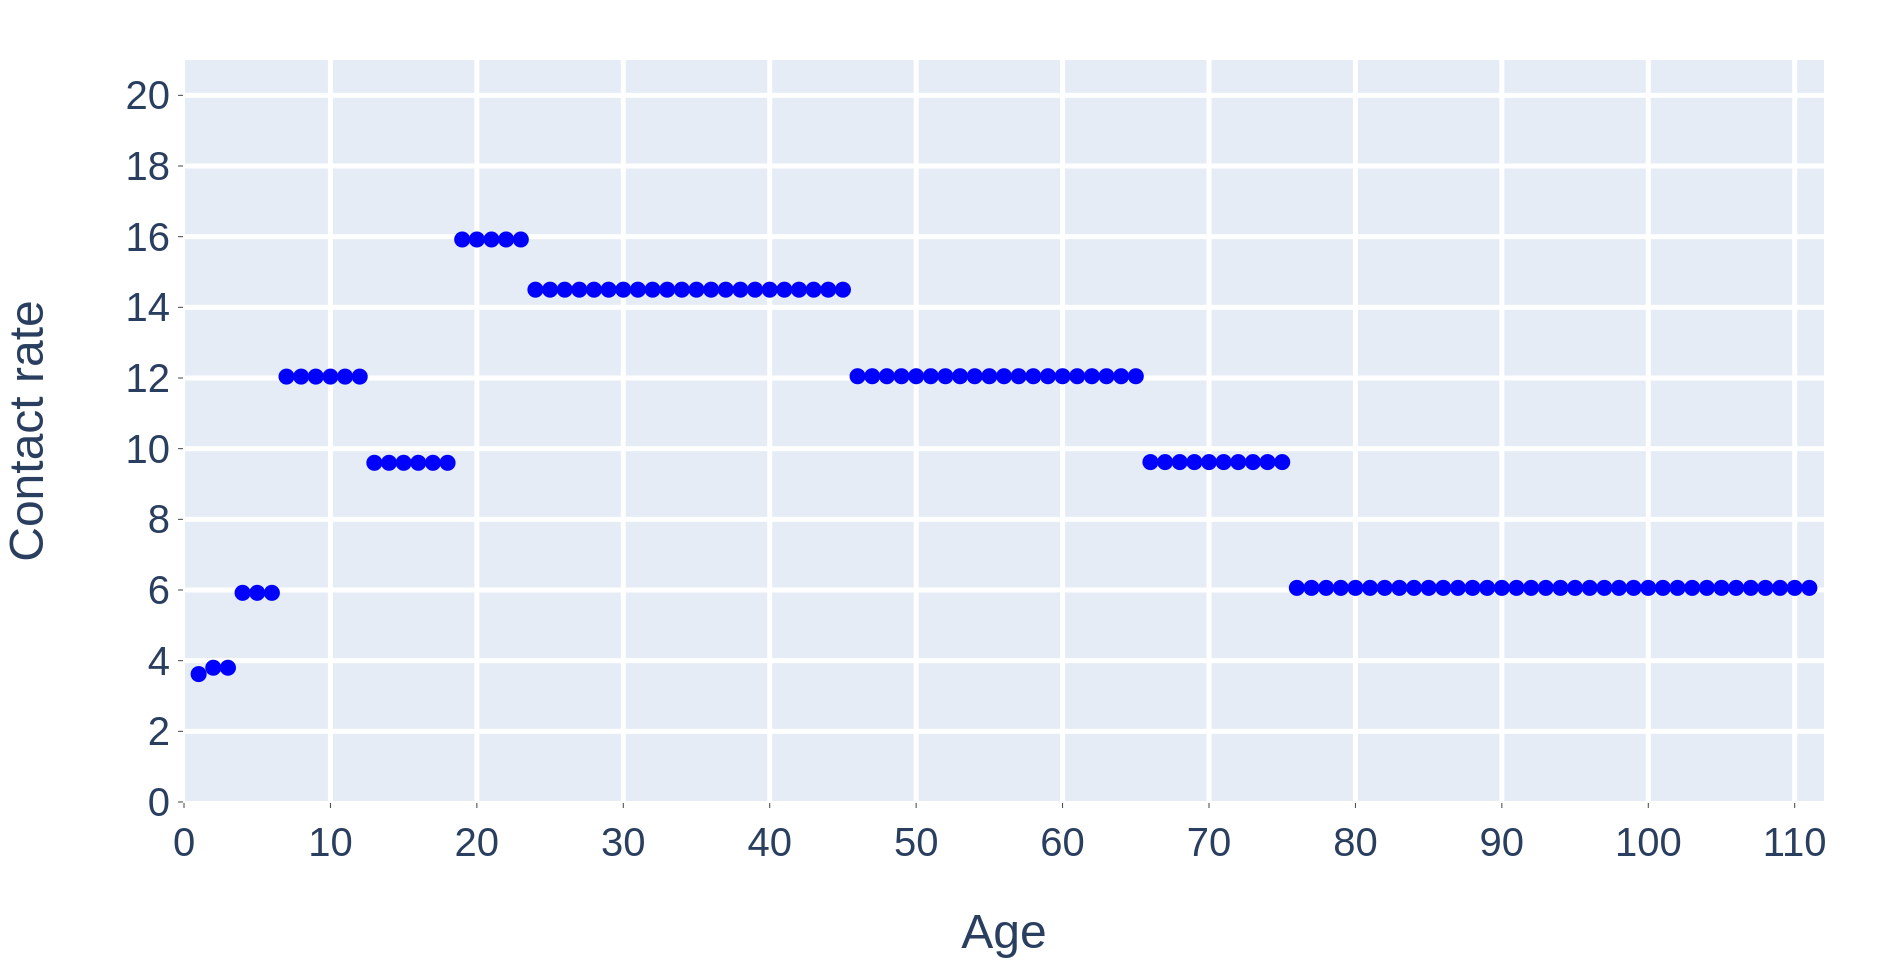
\includegraphics[width=.8\textwidth]{3 - Stride/fig/primary_contact_rates.png}
    \caption{Contact rates per age in a primary community.}
    \label{fig:primary_contact_rates}
\end{figure}

\begin{figure}
    \centering
    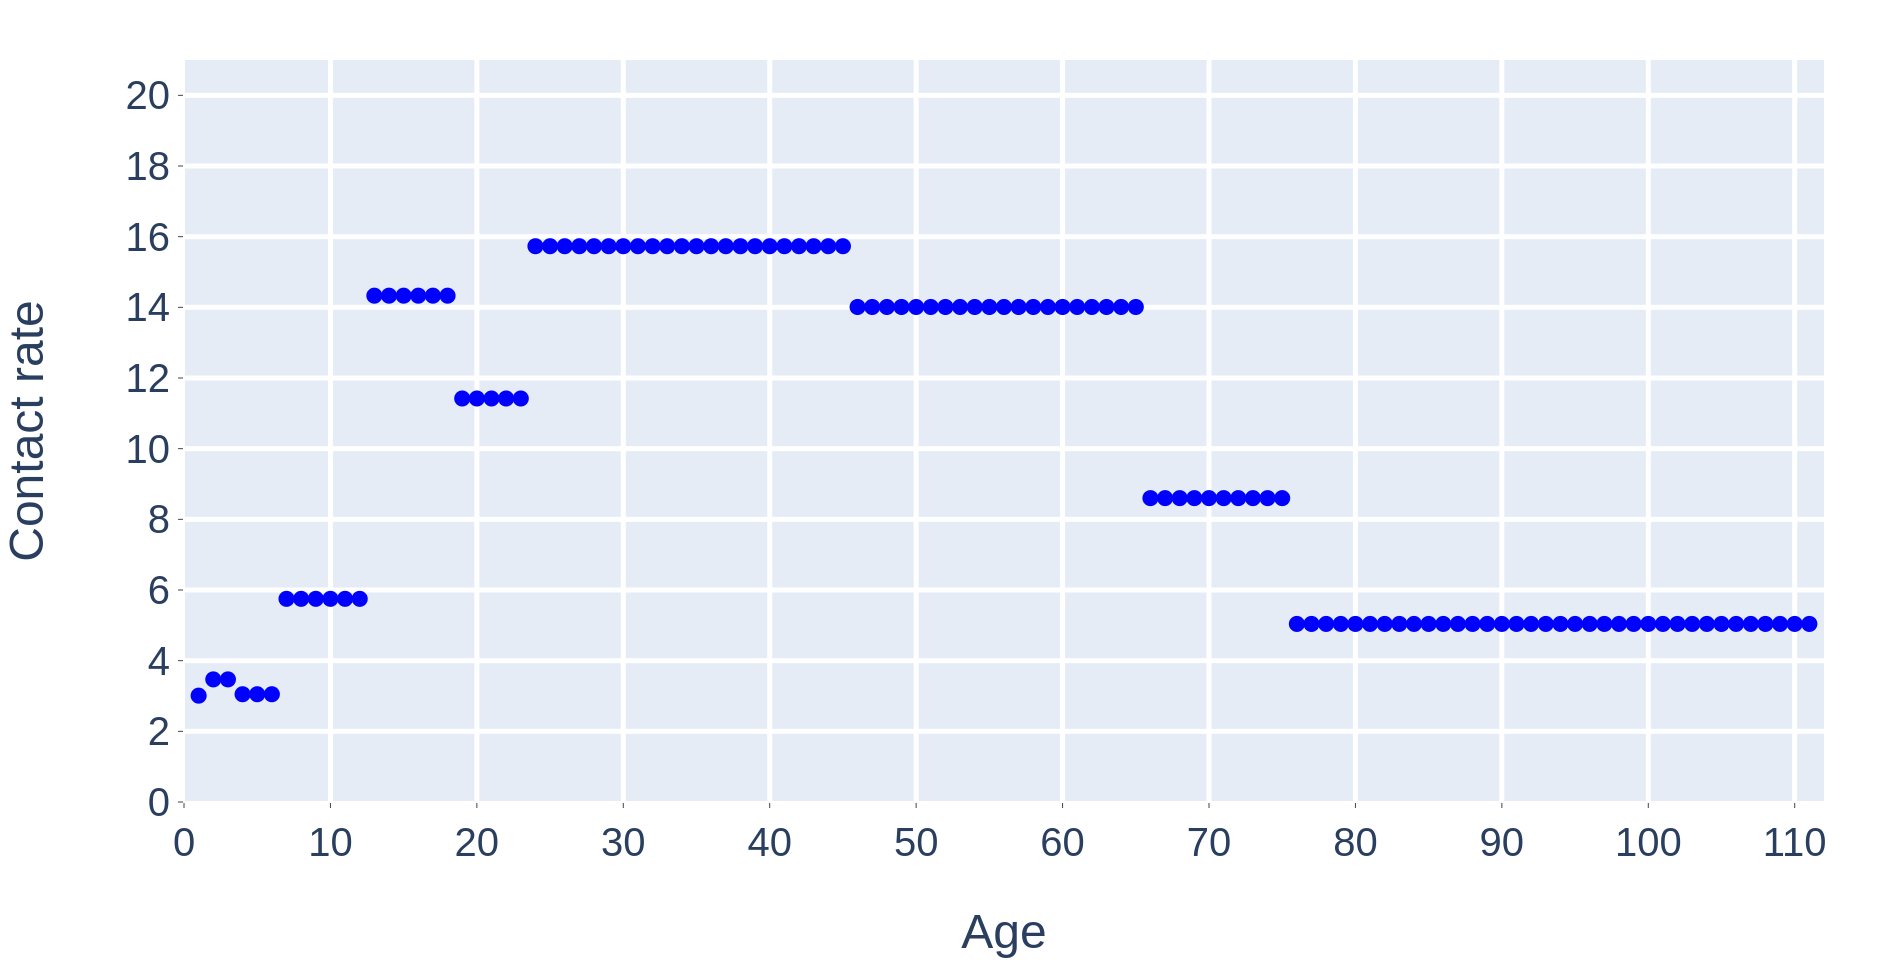
\includegraphics[width=.8\textwidth]{3 - Stride/fig/secondary_contact_rates.png}
    \caption{Contact rates per age in a secondary community.}
    \label{fig:secondary_contact_rates}
\end{figure}

%-------------------------

\begin{figure} 
  \begin{subfigure}[b]{0.45\linewidth}
    \centering
    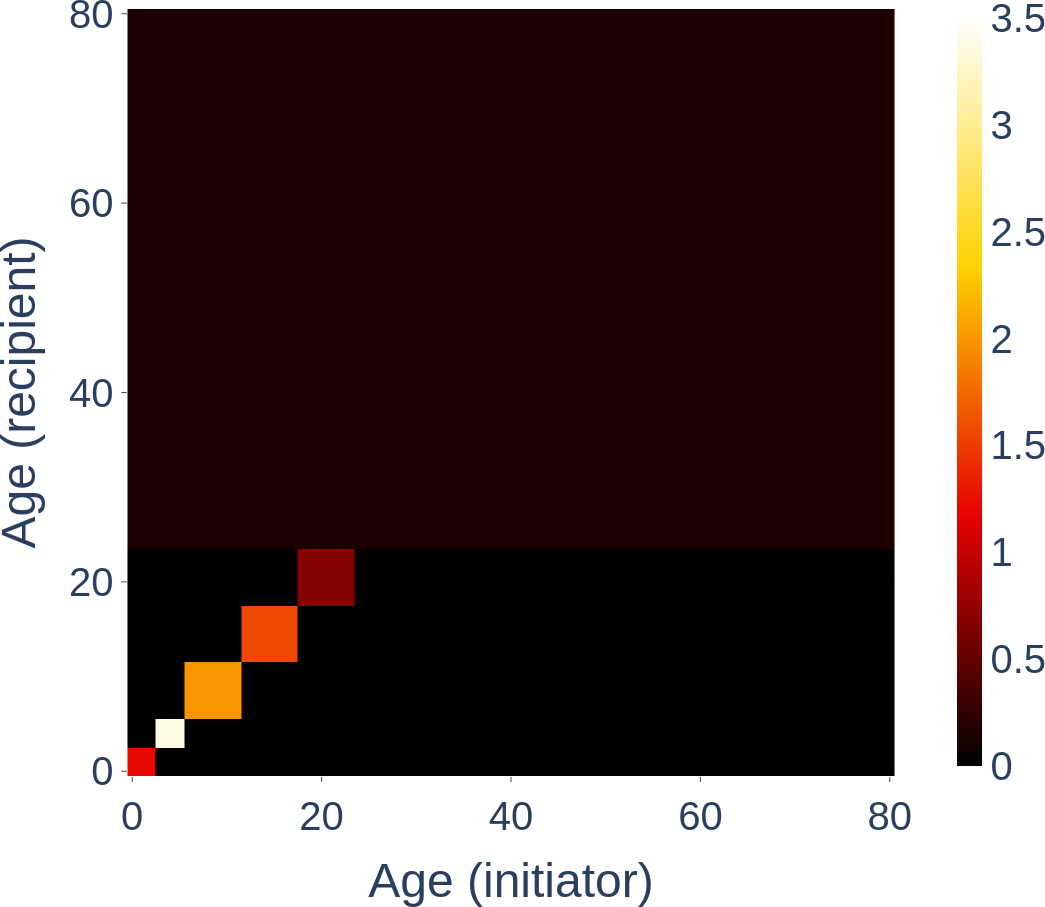
\includegraphics[width=\linewidth]{3 - Stride/fig/school_contact_heatmap.png} 
    \caption{School.} 
    \label{fig:school_contact_heatmap} 
    \vspace{4ex}
  \end{subfigure}%% 
  \hfill
  \begin{subfigure}[b]{0.45\linewidth}
    \centering
    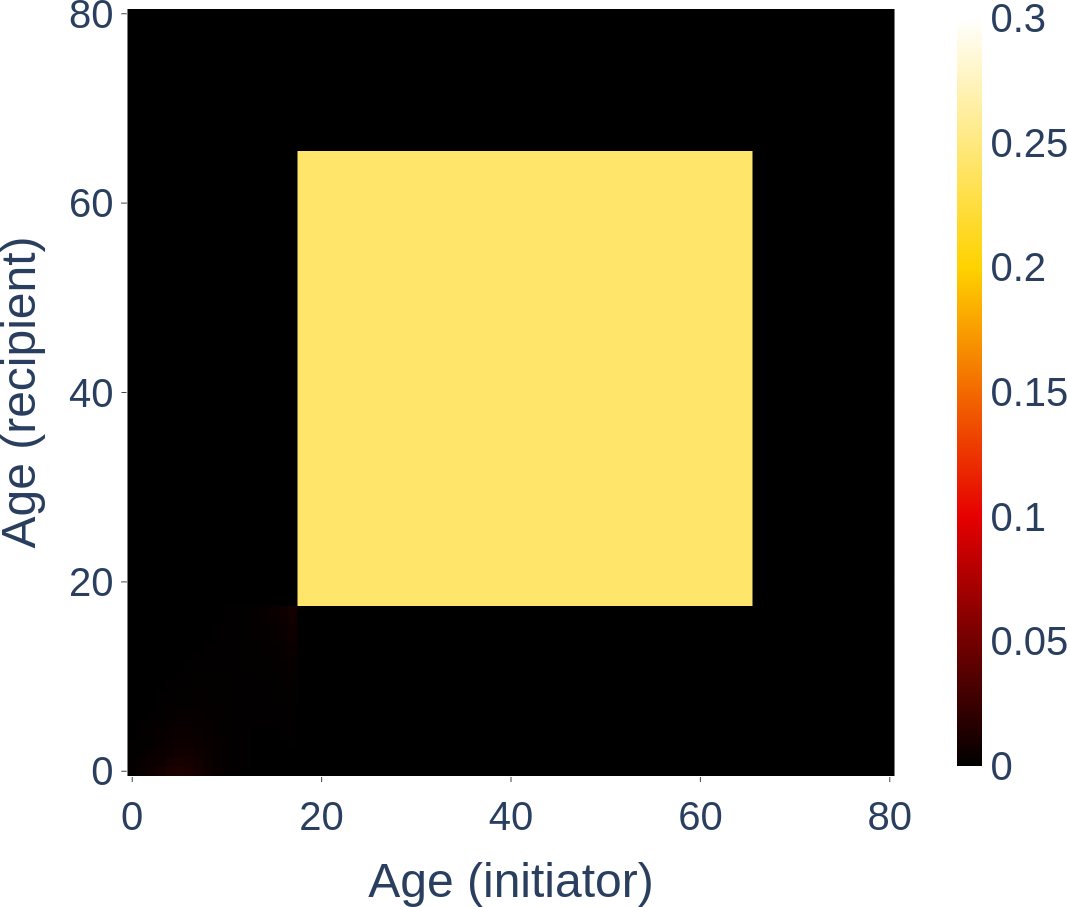
\includegraphics[width=\linewidth]{3 - Stride/fig/work_contact_heatmap.png} 
    \caption{Workplace.} 
    \label{fig:workplace_contact_heatmap} 
    \vspace{4ex}
  \end{subfigure}
  \begin{subfigure}[b]{0.45\linewidth}
    \centering
    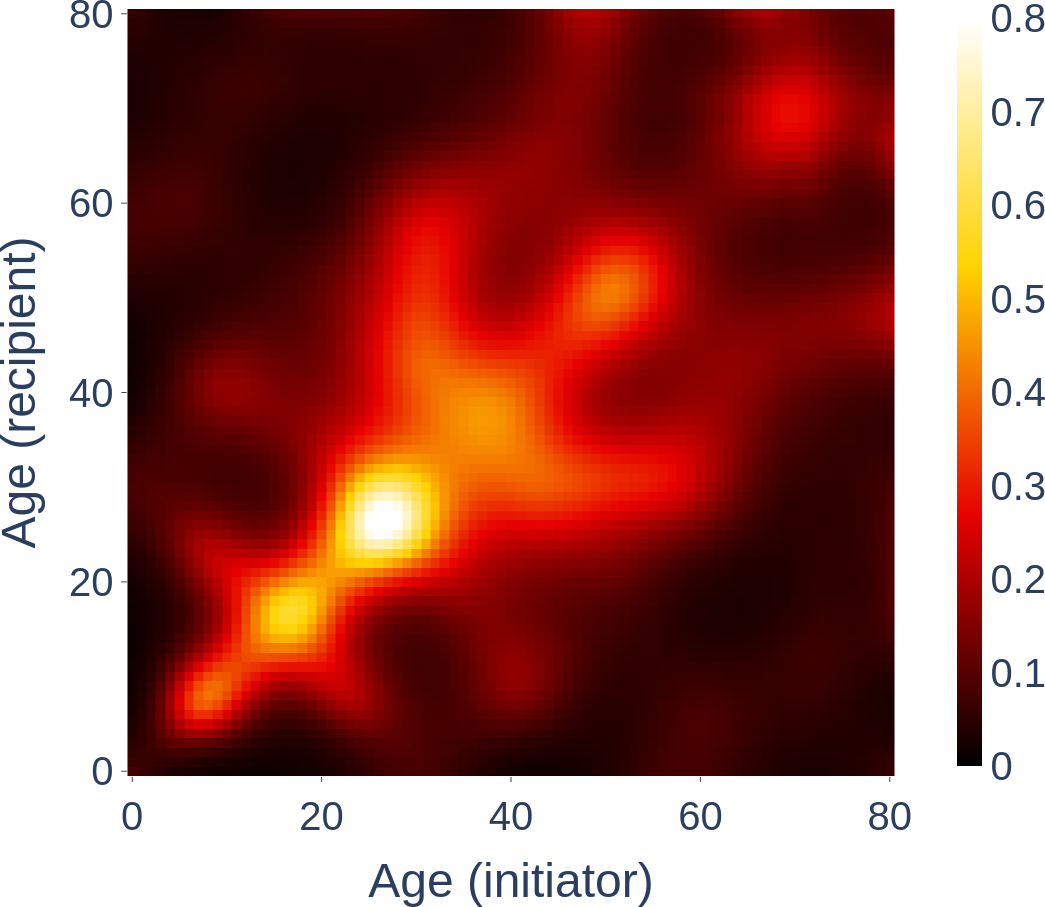
\includegraphics[width=\linewidth]{3 - Stride/fig/primary_contact_heatmap.png} 
    \caption{Primary community.} 
    \label{fig:primary_contact_heatmap} 
  \end{subfigure}%%
  \hfill
  \begin{subfigure}[b]{0.45\linewidth}
    \centering
    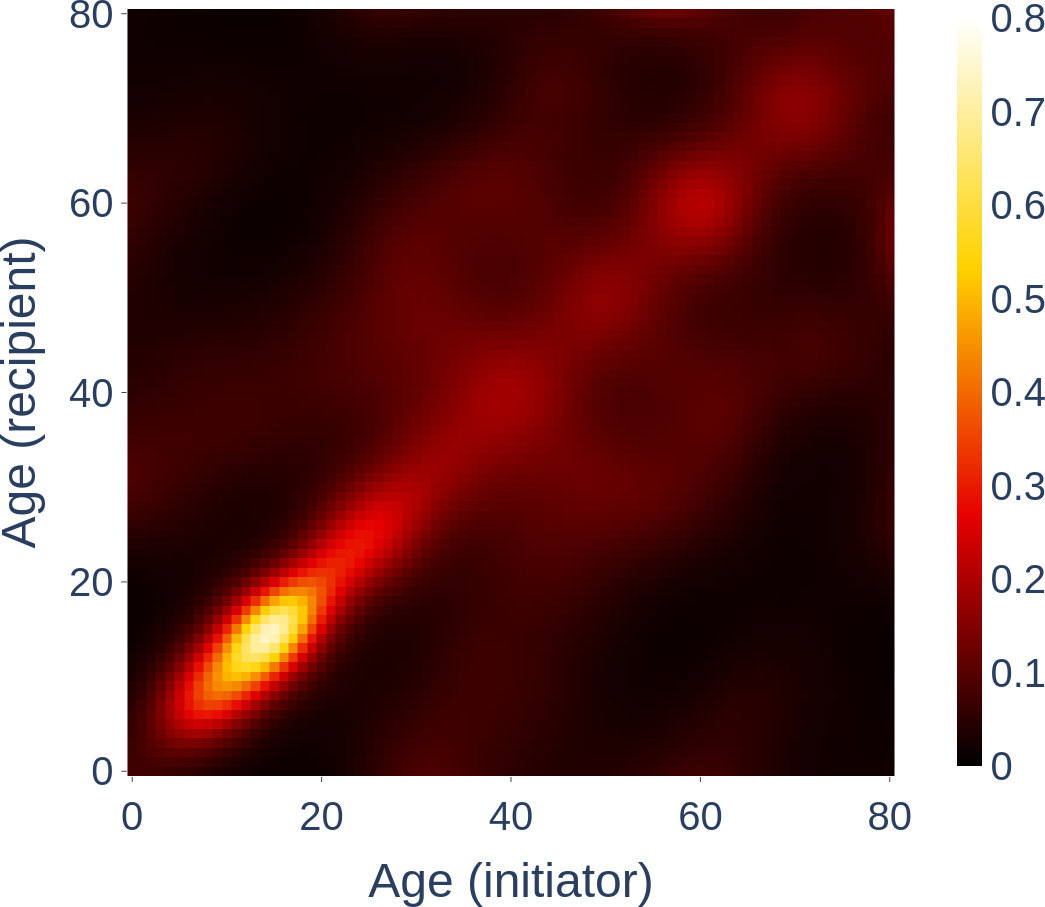
\includegraphics[width=\linewidth]{3 - Stride/fig/secondary_contact_heatmap.png} 
    \caption{Secondary community.} 
    \label{fig:secondary_contact_heatmap} 
  \end{subfigure} 
  \caption{2D contact matrix heatmaps showing the contact rates based on the ages of the contact initiator and recipient.}
  \label{fig:contact_heatmaps} 
\end{figure}

\section{Analysis}
\label{sec:analysis}
Now that we have a complete understanding of Stride, we can dig into the code and start to analyse it. 

\subsection{Parallellization}
A well-known optimisation technique in programming is called \textit{parallellization}, which is the act of executing multiple parts of the program simultaneously. This can only be applied when a program allows for its code to be run in parallel. There are various parallellization techniques and each has its own pros and cons, so which one is most suitable depends on the situation. Stride also uses such a technique and it is called OpenMP\footnote{\url{https://www.openmp.org/}}.
\\\\
In computer science, a thread (of execution) is a term used to describe the smallest sequence of program instructions that can be run independently \cite{multiprocess_programs}. OpenMP is an implementation of multithreading, which is the act of executing multiple threads concurrently and it is managed by the CPU (central processing unit). A thread runs on a core of a CPU and such a core can execute multiple threads concurrently. A core can only execute one thread at a time, so when there are multiple threads that need to be executed by a core, some need to wait their turn. If we were to use multithreading on a single core, the program would become slower instead of faster, because the threads would still be run sequentially and there would be overhead from the CPU who has to manage the threads. CPUs nowadays have multiple cores which allows us to divide the threads on the cores. When we now want to use OpenMP, we need to check the number of cores our CPU has. We then use this number to tell our program the maximum number of threads it can use for the most optimal run time.
\\\\
An important aspect of OpenMP is that CPU cores share their memory. How this memory sharing exactly works depends on the CPU, but these details do not belong to the scope of this thesis. However, this can become an issue when working with a lot of data which, as we will see, is the case for Stride.

\subsection{Code}
In Section \ref{sec:simulation} we explained how a Stride simulation works, which was also visualised in Figure \ref{fig:simulation_flow}. Every part of the simulation process will we now examine separately while we simultaneously think about possible ways to improve the code that we are looking at.

\subsubsection{Initialisation}
We have seen that the initialisation consists of reading the configurations and setting up the simulation accordingly. Most of these configurations are values that have an effect on how the simulation has to run and what information it has to produce, but they only take one hundredth of a second and can thus be ignored. The first major portion is reading the 11M population file, which translates to reading 11 million rows and creating an individual for every single row. This is done in sequence by reading row after row and creating a person every time and storing it in the population. Reading this file could be done in parallel, but trying to store the individuals concurrently in the population would probably cause more harm than good due to the threads that need to store something in the same memory.
\\\\
After the population and contact pools have been created, it is turn to the seeders to determine the individuals' health characteristics, the people who are immune, and the people who start infected. These seeders are already optimised by using OpenMP where possible.

\subsubsection{Updating individuals}
The next step in our code is the update of every individual. This consists of updating a person's health status, as seen in Section \ref{subsec:health_status_update}, and then immediately updating the pools in which the person will be present for the upcoming day, as seen in Section \ref{subsec:pool_presences}. Stride iterates over the entire population and updates every individual separately, but this iteration is implemented with the possibility to use OpenMP. This, together with the fact that the updates are very small functions, indicates that there will probably be not much room to improve Stride here.

\subsubsection{Contact tracing}
As we know from Section \ref{subsec:contact_tracing}, it is possible to use a contact tracing feature in Stride. This code section iterates twice over the population without OpenMP, so this could already be a potential optimisation by parallellizing the iterations. However, because this part of the code does not belong to the standard simulation, we give this section the lowest priority when making improvements. Besides these iterations the contact tracing performs some operations that need to be done and cannot be changed or improved.

\subsubsection{Calculating contacts and transmissions}
Section \ref{subsec:contacts_and_transmissions} explained the core of Stride, which is how contacts and transmissions get calculated. There are two algorithms for this: \textsc{All-to-All} and \textsc{Inf-to-Sus}. Only one of these can be used when simulating a day and this is determined at runtime. They are both implemented in a template called \textit{infector} and how Stride executes this for every pool is shown in Algorithm \ref{alg:infector}, which consists of pseudo code combined with the actual OpenMP calls for completeness. We iterate over all the contact pool types and check if the type of pool is active in the current day and if not, we skip this type of pool. If we are, for example, simulating a holiday, we skip the workplace type. If the type of pool is active, we then iterate over every pool of that type and send them to the infector. During this thesis, several questions and concerns arose about this implementation, which we will now discuss:
\begin{enumerate}
    \item \textbf{We calculate the contacts and transmissions for every pool of every type in one large iteration, how does this affect the results?}
    
    The order in which we do all these calculations does not matter that much. When someone becomes exposed, it always takes at least a day before they get infected or start feeling symptoms. Therefore, they will not be able to infect someone in the same iteration or change their behaviour.
    
    \item \textbf{When we use OpenMP, is there a possibility that problems occur regarding memory read and write operations? For example when two pools are being processed by infector and they consist of overlapping individuals.}
    
    The parallellization only applies to the inner for-loop which iterates over all the pools of a particular type. We have seen that people can only be a member of one pool per pool type, so this rule prevents such issues.
    
    \item \textbf{At line 9 in Algorithm \ref{alg:infector} the population is passed on to infector. Why would this be necessary and does this present problems regarding OpenMP?}
    
    The population is needed in infector because it gets used when calculating the contact probabilities, although we did not explicitly show this in Algorithm \ref{alg:contact_probability}. This does not cause any issues because the population is wrapped in a shared pointer, as we will see in Section \ref{subsec:first_opt_updating_individuals}.
    
    \item \textbf{We learned that the contacts and transmissions depend on randomness. Since randomness has to be created via random number generators, would this not cause problems when using OpenMP?}
    
    In Section \ref{subsec:initialisation} we discussed how random number generator (RNG) managers are the first thing that get created in the initialisation step. Stride creates such RNG managers for every thread and passes these on to infector, as we see in line 9 of Algorithm \ref{alg:infector}, which takes care of any issues regarding random number generators with multithreading.
\end{enumerate}

\begin{algorithm}
\caption{Pseudo code of how \textit{infector} is used on every pool in a simulation day.}
\label{alg:infector}
\begin{algorithmic}[1]
    \State \textbf{\#pragma} omp parallel num\_threads(m\_num\_threads)
    \State \{
    \State $thread\_num \gets$ \Call{omp\_get\_thread\_num}{\null}
    \Foreach{$type$ in  $pooltypes[\;]$} \Comment{Iterate over pool types}
        \If{$type$ not active}
            \State continue \Comment{Ignore this type and go to the next}
        \EndIf
        \State \textbf{\#pragma} omp for schedule(static)
        \Foreach{$pool$ in $pools[type]$} \Comment{Iterate over every pool of $type$}
            \State \Call{infector}{$pool, population, rng\_handler[thread\_num], ...$}
        \EndForeach
    \EndForeach
    \State \}
\end{algorithmic}
\end{algorithm}

\subsection{Performance}
\label{subsec:performance}
A first code examination of Stride taught us more about the different components of the program and how parallellization is already used to improve the simulation speed. Our next step is to run the simulation with different parameters and measure the performance. All simulations in this chapter and the next use the configurations described in Appendix \ref{appendix:configurations} unless stated otherwise. \paragraph{VSC} All of the following tests in this chapter and Chapter \ref{chapter:sampling} ran on the VSC\footnote{\url{https://www.vscentrum.be/}} (Vlaams Supercomputer Centrum, or in English Flemish Supercomputer Centre) to get the most optimal results with the least amount of external interference. Our tests ran on (cascadelake) computer nodes with a Xeon Gold 6240 CPU@2.6 GHz with 18 cores; 192 GB RAM; 200 GB SSD local disk. \textsc{All-to-All} simulations have memory and virtual memory peaks of respectively 9.5 GB and 10.2 GB, while \textsc{Inf-to-Sus} only has peaks of 3.1 GB memory and 3.3 GB virtual memory. Memory bandwidth and latency measurements can be found on the VSC website\footnote{\url{https://docs.vscentrum.be/en/latest/leuven/tier2_hardware/memory_bandwidth_and_latency_tier2.html\#memory-bandwidth-and-latency-cascadelake-tier2}}.
\\\\
For our performance tests we divide the model in three sections and measure the time of each section as well as the total time. The sections are: updating individuals, contact tracing, and calculating contacts and transmissions (which we will now refer to as infector). With our first test, we want to see how much time Stride spends per section each day for both infector algorithms. The results for these simulations using \textsc{All-to-All} and \textsc{Inf-to-Sus} are visualised in Figure \ref{fig:basis_runtime_sections}. The average results per section are listed in Table \ref{tab:basis_runtime_stats}. The small runtime differences, such as the updating and tracing sections for both algorithms, are due to low-level system details and are negligible for the rest of this thesis.
\\\\
We notice from our results that the \textsc{Inf-to-Sus} is a major runtime optimisation compared to \textsc{All-to-All}, which is all due to the difference in the infector algorithm. When Stride uses \textsc{All-to-All}, almost all of its time is spend in the infector, so this is where we should look for improvements first. The ups and downs that we see in both graphs are caused by the type of day, 5 weekdays and 2 weekend days, where the weekdays take a little bit more time. This is a logical effect because the weekdays have more active pools (household, work, K-12 school, college, and secondary community) than weekend days (household, primary community).
\\\\
\textsc{Inf-to-Sus} displays a somewhat normal distribution regarding the infector time, with a peak around day 50. The explanation for this behaviour is that the infector only gets executed for a pool when at least one of its member is infectious. Figure \ref{fig:basis_infected} shows the number of people who are infected per simulation day. The number of people who are infected clearly matches these changes in runtime of the infector. The first day of this simulation also takes a lot more time than the following days, which is due to the sorting of the individuals based on their health status. At the start, these pools are initialised without sorting the members and thus it takes more time to sort them. When they get sorted the next day, there only need to be a few changes made on average which causes the sorting to be much faster.
\\\\
The total runtime of the entire 100-day simulation using \textsc{All-to-All} lasted 1 hour 43 minutes and 32 seconds, of which the initialisation took approximately 1 minute. The \textsc{Inf-to-Sus} simulation obviously needed the same amount of time for the initialisation, but ran in a total time of 5 minutes and 49 seconds. \textsc{Inf-to-Sus} only does calculations that are absolutely necessary and has therefore very little room for improvement compared to \textsc{All-to-All}. Our focus will thus not lie on the initialisation, because it is only a small percentage of the simulation when using \textsc{All-to-All}. Contact tracing needs the least amount by far, so we ignore this part from now on and will only mention it sometimes for the sake of completeness.

\begin{figure}
    \centering
      \begin{subfigure}[b]{\linewidth}
        \centering
        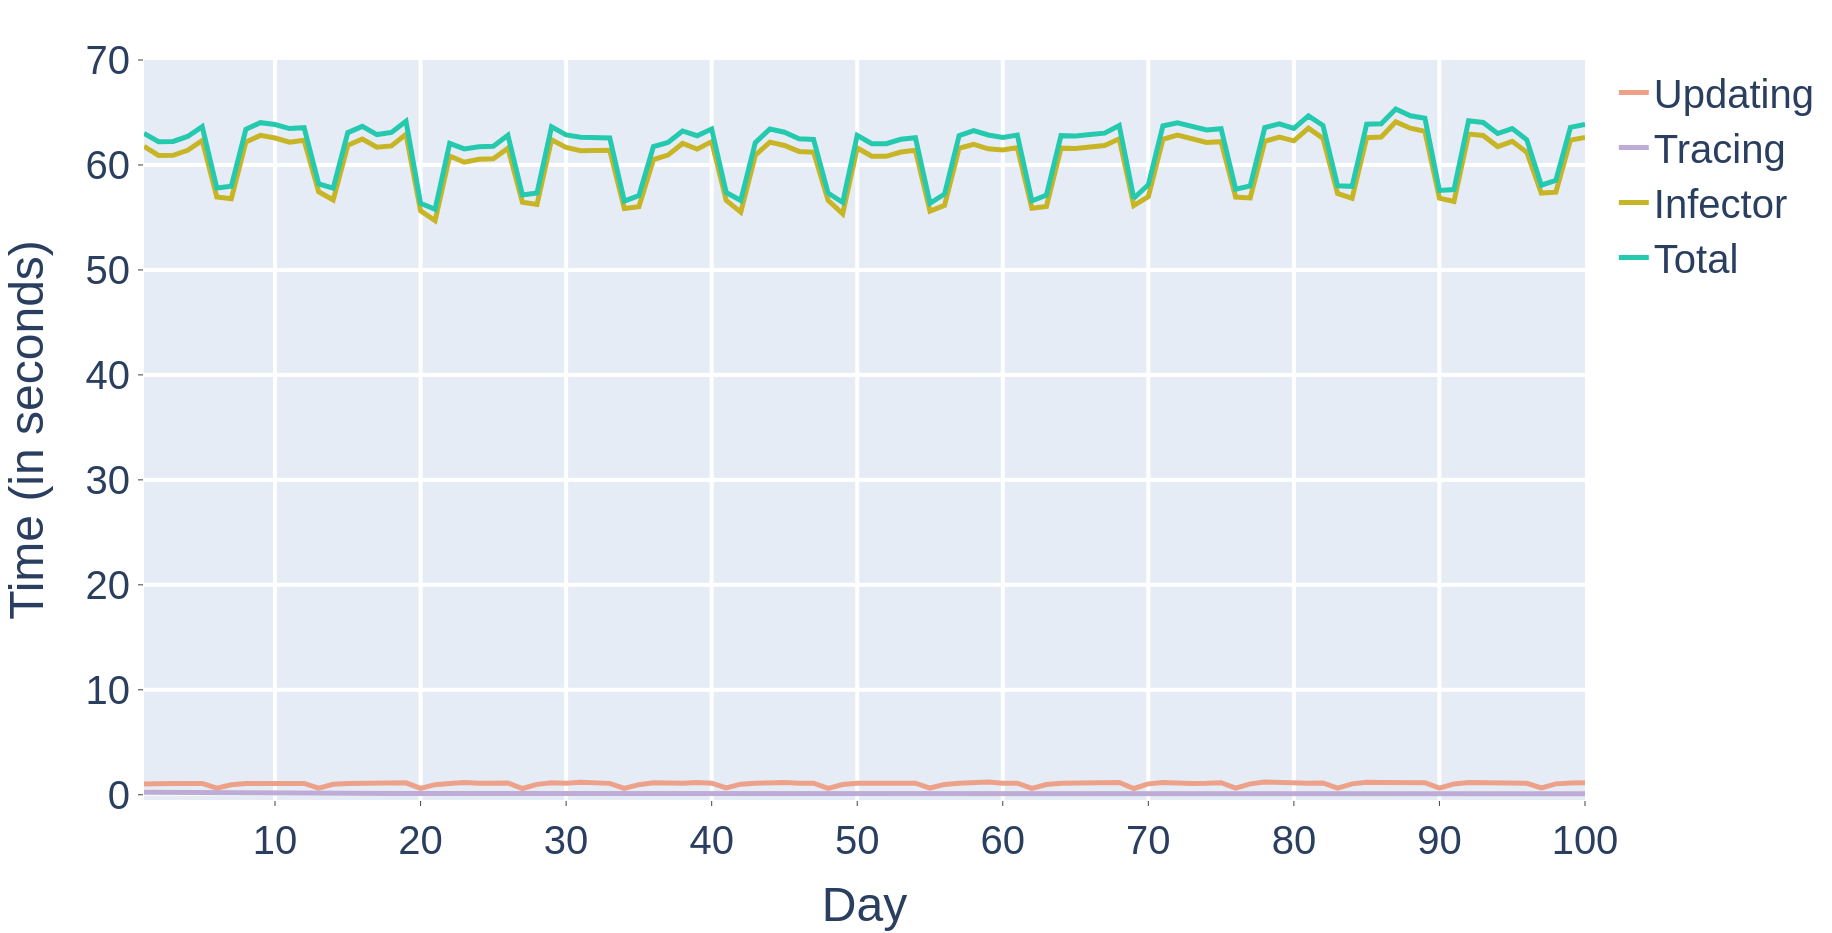
\includegraphics[width=\linewidth]{3 - Stride/fig/basis_all_runtime_sections.png} 
        \caption{\textsc{All-to-All}.} 
        \label{fig:basis_all_runtime_sections} 
      \end{subfigure}
      \begin{subfigure}[b]{\linewidth}
        \centering
        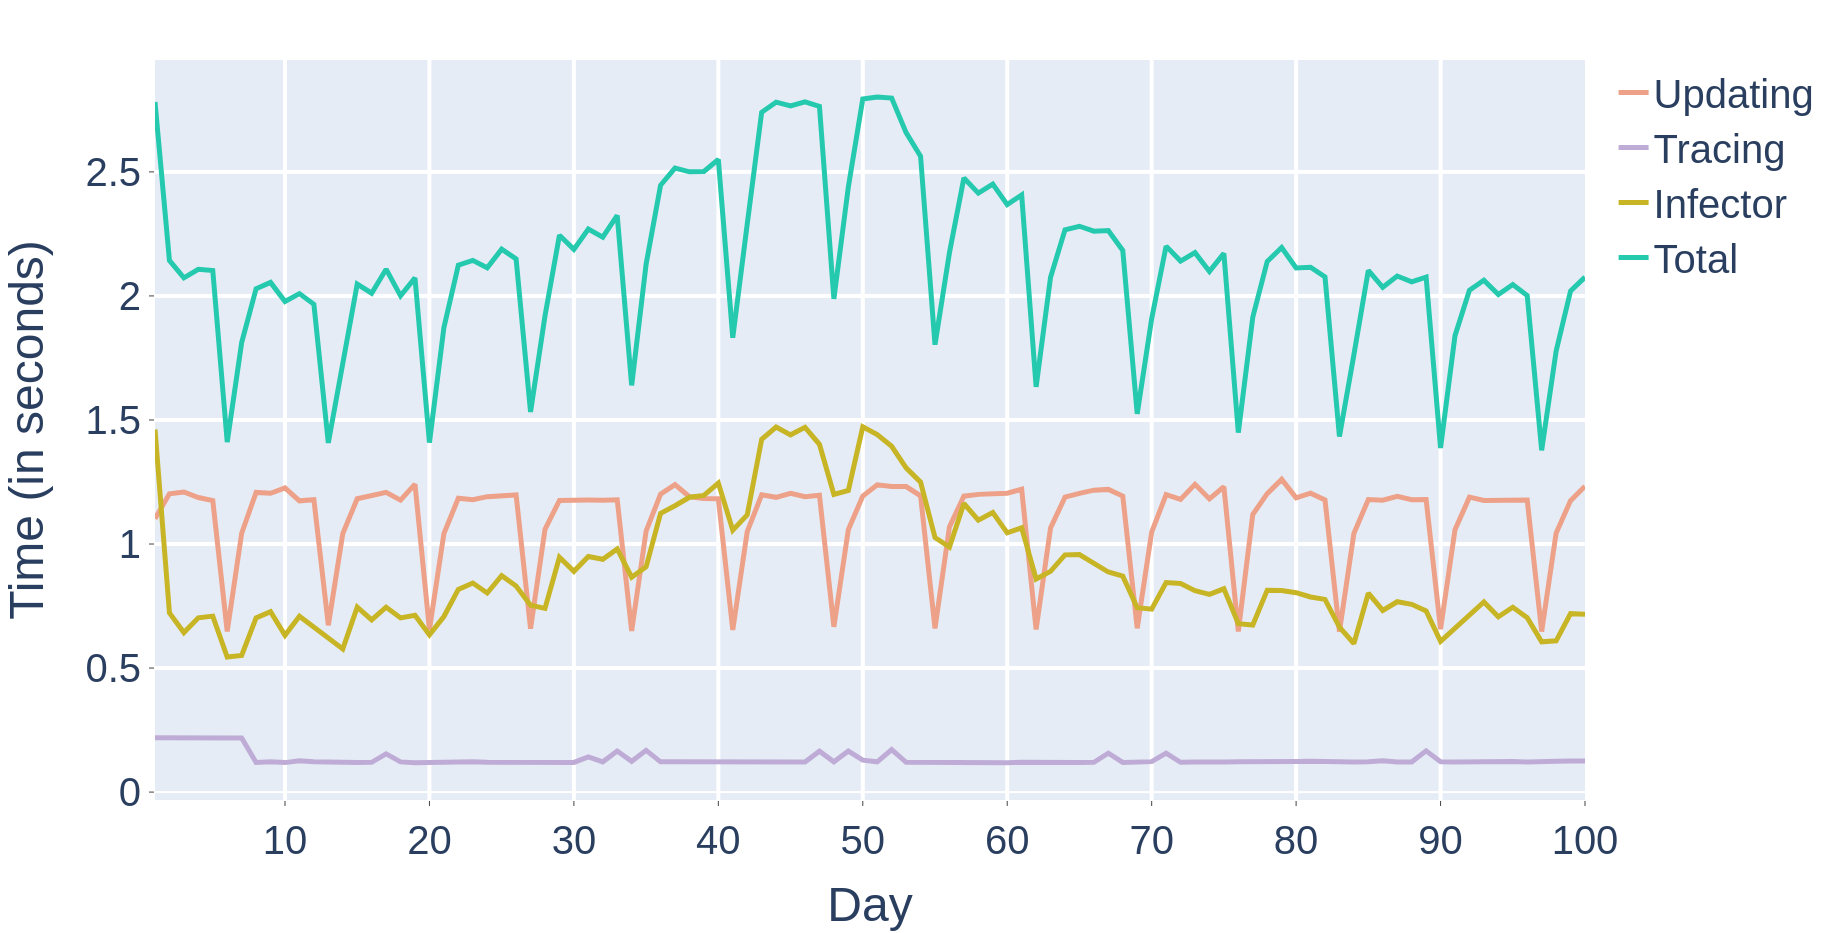
\includegraphics[width=\linewidth]{3 - Stride/fig/basis_opt_runtime_sections.png} 
        \caption{\textsc{Inf-to-Sus}.} 
        \label{fig:basis_opt_runtime_sections} 
      \end{subfigure} 
      \caption{Section times per day, in seconds, for every section, including the total times for simulating a day. Simulations run on 11M population for 100 days without holidays using 1 thread (configurations in Appendix \ref{appendix:configurations}).}
      \label{fig:basis_runtime_sections} 
\end{figure}

\begin{figure}
    \centering
    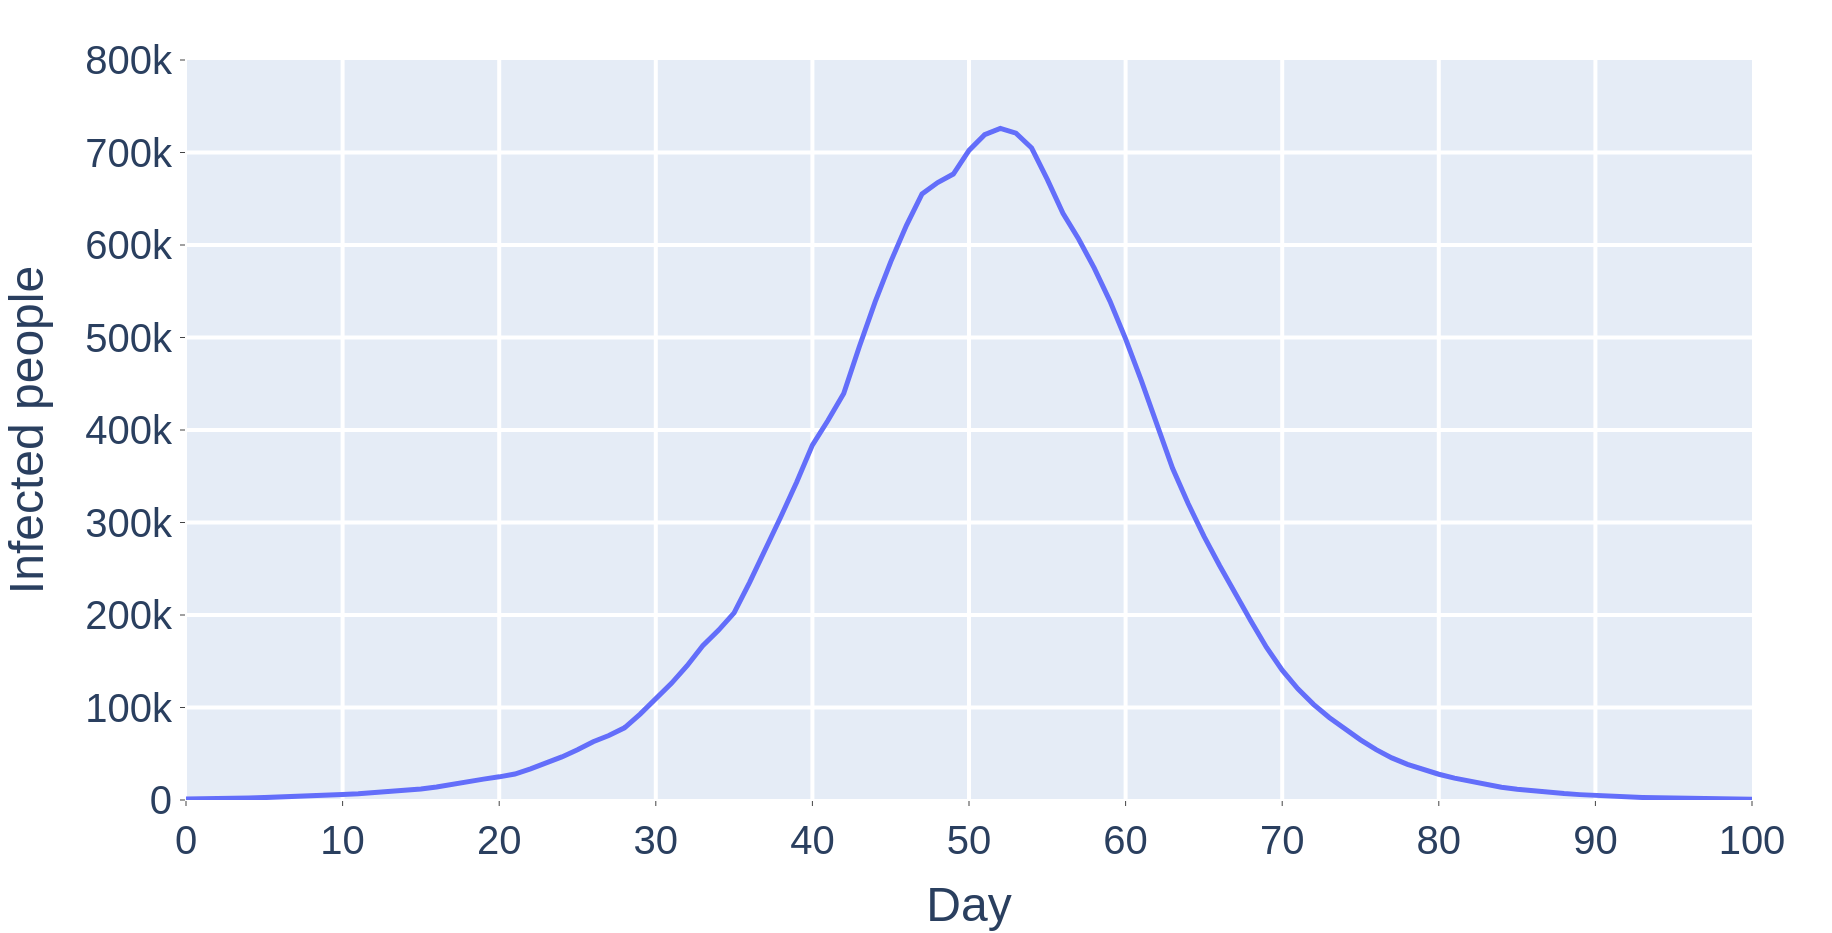
\includegraphics[width=.8\linewidth]{3 - Stride/fig/basis_infected.png}
    \caption{Number of infected people per simulation day. Simulation run on 11M population for 100 days without holidays using 1 thread (configurations in Appendix \ref{appendix:configurations}).}
    \label{fig:basis_infected}
\end{figure}

\begin{table}
\centering
\begin{tabular}{@{}lrrrr@{}}
\toprule
           & Updating & Tracing & Infector & Total \\ \midrule
All-to-All & 1.03     & 0.11    & 60.37    & 61.52 \\
Inf-to-Sus & 1.10     & 0.13    & 0.89     & 2.12  \\ \midrule
speedup    & /        & /       & 67.83    & 29.02 \\ \bottomrule
\end{tabular}
\caption{Average daily runtime (in seconds) per section. Simulations run on 11M population for 100 days without holidays using 1 thread (configurations in Appendix \ref{appendix:configurations}).}
\label{tab:basis_runtime_stats}
\end{table}

\subsubsection{Parallellization}
The next test that we will perform is to see how the previously implemented parallellization affects the runtimes, given that Stride is regularly expanded and updated, which could have harmed the parallellization performance. For this part, we will only focus on the parts of a simulation day that use OpenMP, which are the updating of individuals and the calculations of contacts and transmissions. Figure \ref{fig:basis_parallel_updating} reveals how the updating of individuals becomes slower when using more threads instead of faster. The implementation of OpenMP, which is supposed to be an improvement, has the opposite effect. We see a similar trend when looking at the \textsc{All-to-All} infector in Figure \ref{fig:basis_all_parallel_infector}. Here we notice that using two threads is the slowest and that using more threads than becomes gradually faster, although it is still much slower than the simulation without parallellization. The \textsc{Inf-to-Sus} infector exhibits rather strange behaviour regarding parallellization, which we can see in Figure \ref{fig:basis_opt_parallel_infector}. Using multiple threads is faster in the beginning and at the end of the simulation, but is slower in between. \textsc{Inf-to-Sus} has, just like \textsc{All-to-All}, the slowest times when using two threads and starts to become faster if more threads are used.
\\\\
In order to be more accurate, the average times per simulation day for all of these parallellization tests are displayed in Table \ref{tab:basis_parallel}. This confirms our statements about updating individuals and the \textsc{All-to-All} infector parallellization, but shows that multithreading is in fact faster on average for the \textsc{Inf-to-Sus} infector. However, the total simulation time is still higher when using multiple threads because of the updating of individuals.

\begin{figure}
    \centering
    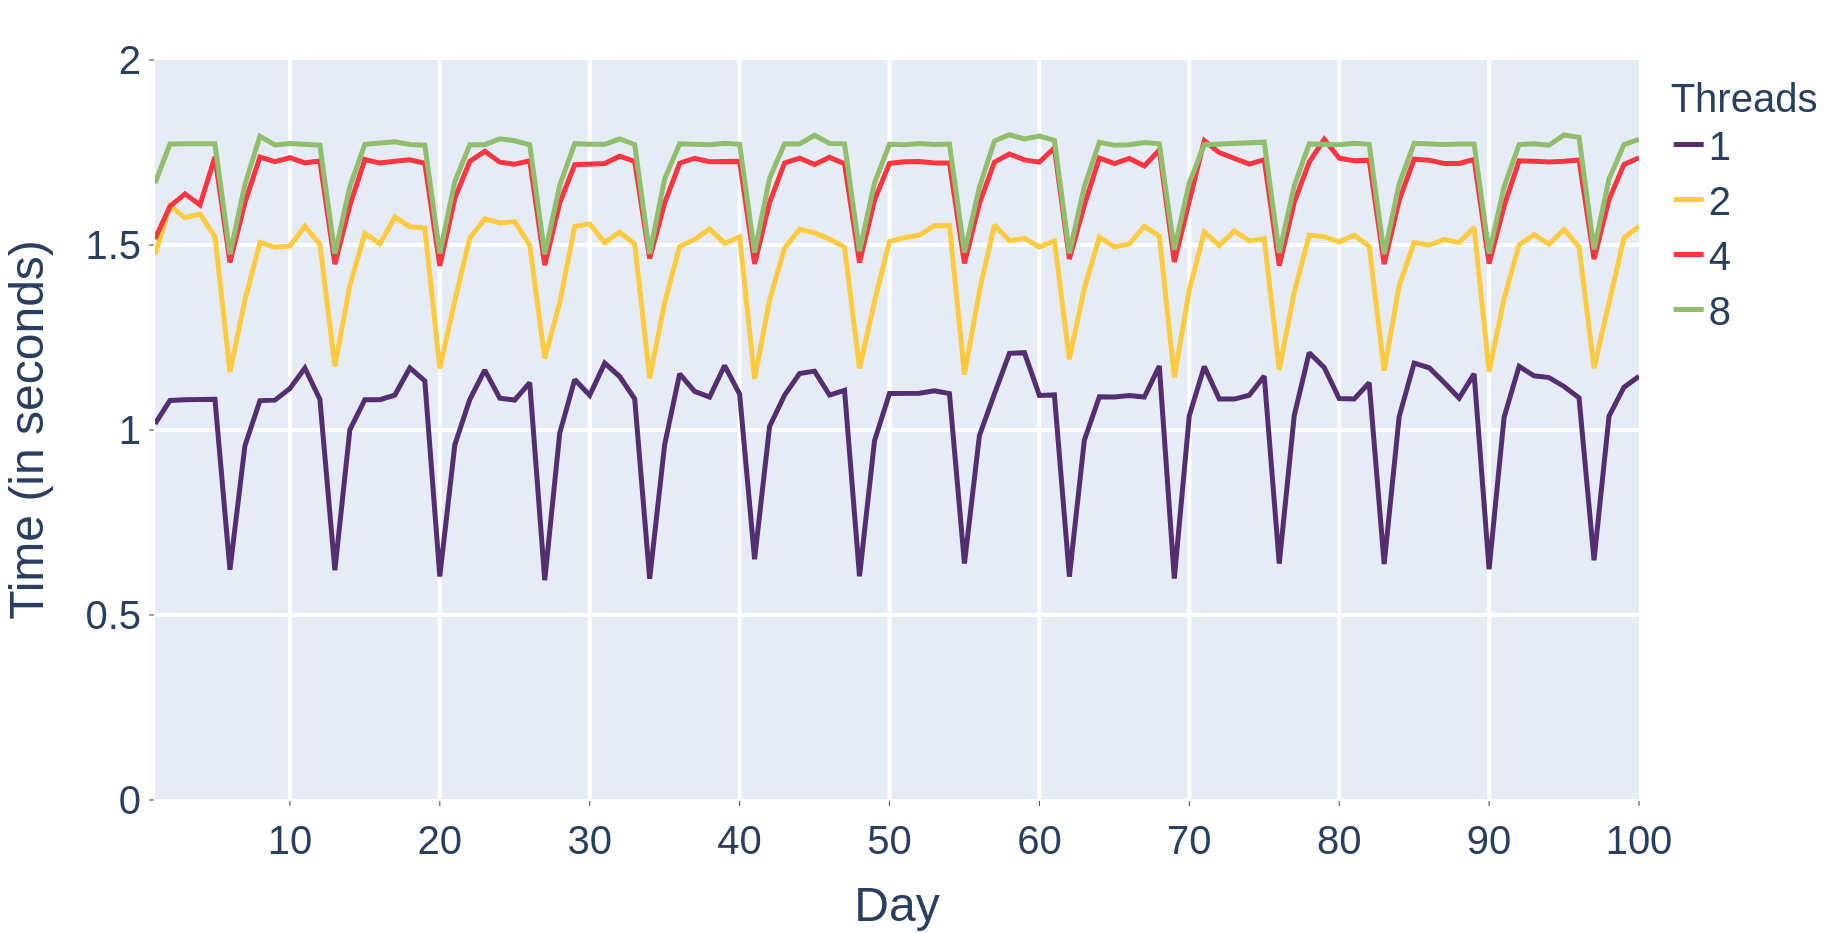
\includegraphics[width=\linewidth]{3 - Stride/fig/basis_parallel_updating.png}
    \caption{Time per simulation day for updating individuals using different number of threads. Simulations run on 11M population for 100 days without holidays (configurations in Appendix \ref{appendix:configurations}).}
    \label{fig:basis_parallel_updating}
\end{figure}

\begin{figure}
    \centering
    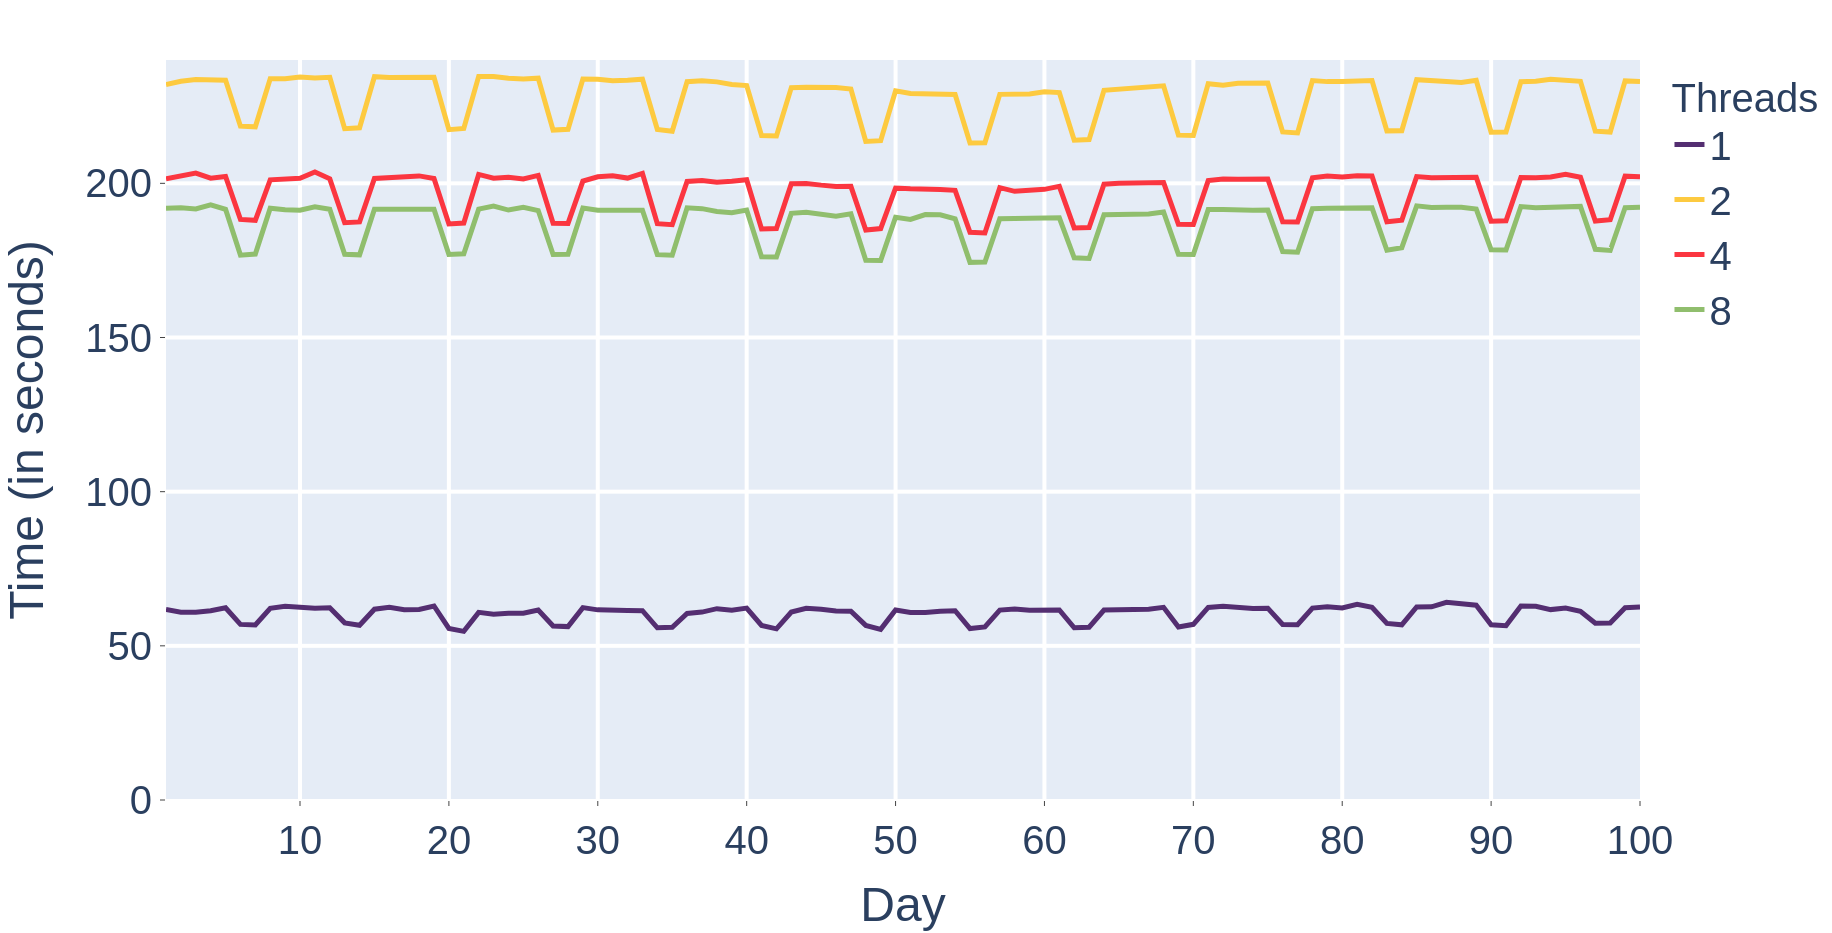
\includegraphics[width=\linewidth]{3 - Stride/fig/basis_all_parallel_infector.png}
    \caption{Time per simulation day for the infector using \textsc{All-to-All} using different number of threads. Simulations run on 11M population for 100 days without holidays (configurations in Appendix \ref{appendix:configurations}).}
    \label{fig:basis_all_parallel_infector}
\end{figure}

\begin{figure}
    \centering
    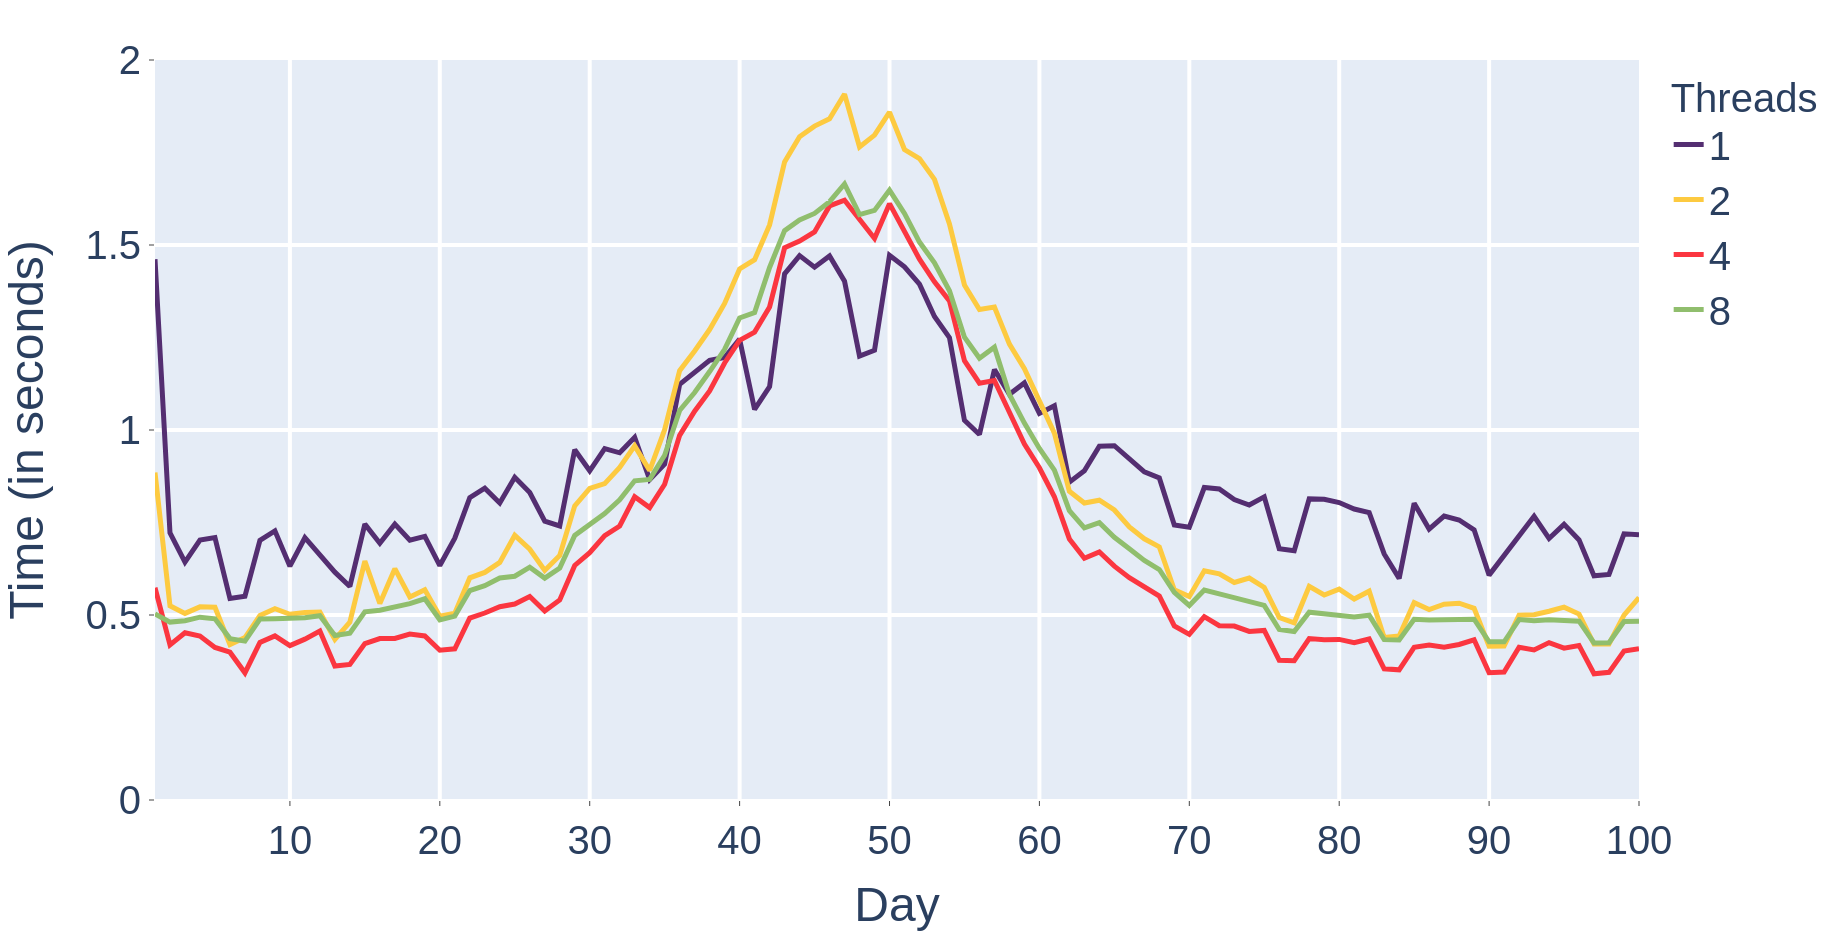
\includegraphics[width=\linewidth]{3 - Stride/fig/basis_opt_parallel_infector.png}
    \caption{Time per simulation day for the infector using \textsc{Inf-to-Sus} using different number of threads. Simulations run on 11M population for 100 days without holidays (configurations in Appendix \ref{appendix:configurations}).}
    \label{fig:basis_opt_parallel_infector}
\end{figure}

\begin{table}
    \begin{subtable}[h]{0.45\textwidth}
        \centering
        \begin{tabular}{@{}crrr@{}}
            \toprule
            Threads & Updating & Infector & Total  \\ \midrule
            1       & 1.08     & 64.33    & 65.56  \\
            2       & 1.45     & 227.93   & 229.50 \\
            4       & 1.67     & 197.04   & 198.85 \\
            8       & 1.72     & 187.15   & 189.00 \\ \bottomrule
        \end{tabular}
        \caption{\textsc{All-to-All}.}
        \label{tab:basis_all_parallel}
    \end{subtable}
    \hfill
    \begin{subtable}[h]{0.45\textwidth}
        \centering
        \begin{tabular}{@{}crrr@{}}
            \toprule
            Threads & Updating & Infector & Total \\ \midrule
            1       & 1.10     & 0.89     & 2.12  \\
            2       & 1.52     & 0.83     & 2.48  \\
            4       & 1.66     & 0.69     & 2.49  \\
            8       & 1.67     & 0.75     & 2.57  \\ \bottomrule
        \end{tabular}
        \caption{\textsc{Inf-to-Sus}.}
        \label{tab:basis_opt_parallel}
    \end{subtable}
    \caption{Average daily runtime (in seconds) per section. Simulations run on 11M population for 100 days without holidays (configurations in Appendix \ref{appendix:configurations}).}
    \label{tab:basis_parallel}
\end{table}

\section{First optimisation}
\label{sec:first_optimisation}
In this section we examine the parallellization problem in depth and present our first major optimisation.

\subsection{Code architecture}
Before we go into details about Stride, we need to disclose the architecture of the code. We will need this information when we need to contemplate about what causes these performance issues.

\subsubsection{Population}
Representing 11 million individuals is, needless to say, a lot of data that has to be stored and managed. Stride uses a segmented vector for its population, which is a container that stores objects, which are individuals in our case, almost contiguously in a chain of blocks. The block size, which is set to 2048, determines how many individuals get stored consecutively. It is designed this way to have better performance regarding CPU caching.

\subsubsection{Person}
Every individual is represented in a \textit{Person} object. This object contains various information such as its ID and age, but also of which pools they are a member and in which they are currently present. Information about their health is stored in another \textit{Health} object. This health object stores the person's health status as well as their health characteristics.

\subsubsection{Shared pointer}
The \textit{Population} is wrapped in a \textit{std::shared\_ptr}. This is a smart pointer designed to facilitate the managing of storage of an object pointer when there are multiple owners that manage its lifetime \cite{shared_ptr_doc}. The underlying structure has a reference counter which keeps track of all instances of the shared pointer and deletes the memory source and itself when this counter reaches zero \cite{shared_ptr_doc_microsoft}.

\subsection{Updating individuals}
\label{subsec:first_opt_updating_individuals}
First we look at the updating of individuals, which needs more time to complete the more threads that are being used. In Sections \ref{subsec:health_status_update} and \ref{subsec:pool_presences} we discussed how every individual gets updated at the start of a simulation day regarding their health status and their pool presences. This is implemented with a single iteration over the entire population in which it calls the \textit{update} function of a Person. The examination of this code does not present any visible errors. A possible reason for the multithreading problem could be related to the memory management done by the CPU. If we want to solve this, there is a strong possibility that we need to do extensive research on this topic and maybe redesign a great portion of the code, which lies outside the scope of this thesis. For this reason and because this section requires only a small portion of the total simulation time, we will ignore this section for now.
\\\\
Let it be stated that we only made assumptions here by looking at the code. We did not perform tests on this section because of the little impact it would have on the total runtime. There is always the possibility to turn of the multithreading for this section, which would still result in acceptable runtimes.

\subsection{Infector}
\label{subsec:first_opt_infector}
We learned that it costs substantially more time for the infector when we use multiple threads and that the \textsc{Inf-to-Sus} infector displays a strange phenomenon, as seen in Figure \ref{fig:basis_opt_parallel_infector}, where multithreading can be both faster and slower depending on the day. We already said that the curve of the \textsc{Inf-to-Sus} infector graph is connected to the number of people who are infected. When there are only a few infected people, the infector from Algorithm \ref{alg:inf-to-sus} then can skip a lot of pools that do not contain an infected member. When multiple threads are being used in the days with a few infections, the infector for \textsc{Inf-to-Sus} is faster than without multithreading. For these reasons we can conclude that the parallellization with OpenMP works well to distribute the infector calls amongst the threads, as seen in Algorithm \ref{alg:infector}, and that the fault probably lies in the \textsc{Inf-to-Sus} code.

\subsection{Solution}
\label{subsec:first_opt_solution}
After detailed examination of both infector algorithms and performing tests, we noticed that most of the infector time was spent for calculating the contact probabilities. When we looked at the code for this function, for which the pseudo code is shown in Algorithm \ref{alg:contact_probability}, we noticed that the population is also a parameter. The reason that this function costs so much time, was because the \textit{shared\_ptr} of this population was being passed by value. In C++, when a parameter is passed by value, a copy of that parameter is created in memory and passed on instead of the original. This is useful when we want to make sure that the function does not change the original data. However, this means that in our case a copy of the \textit{shared\_ptr} of the population needs to be created every time we want to calculate a contact probability. Let it be clear that this is not the same as copying the population itself, but only the \textit{shared\_ptr}.
\\\\
A copy of a normal pointer in C++ would not cause much trouble, because it is only a reference number to the data it points to. When a \textit{shared\_ptr} or a copy of it gets created or destroyed, the reference counter of the shared pointer needs to be updated, which causes some overhead \cite{shared_ptr_doc_microsoft}. The calculation of the contact probability is called for every pair of individuals in \textsc{All-to-All} and for every infectious and susceptible pair in \textsc{Inf-to-Sus} in a pool. Since there is a gigantic amount of pools that need to be passed on to infector, this results in innumerous contact probabilities that need to be calculated and thus results in a lot of overhead. A secondary issue is that the updating of the \textit{shared\_ptr} reference counter is an atomic operation, which means that when a thread needs to update it, it blocks other blocks from accessing this reference counter. Because of this, all the other threads have to wait their turn so that they can update the counter before continuing their thread of execution. This means that there is even more overhead when we use multiple threads for the infector \cite{shared_ptr_doc_microsoft}.
% https://stackoverflow.com/questions/22295665/how-much-is-the-overhead-of-smart-pointers-compared-to-normal-pointers-in-c
\\\\
The solution for all of this is to change the code so that the \textit{shared\_ptr} population is passed by reference instead of by value. This will only create a reference to the shared pointer instead of creating a new one. When a value is passed by reference, the function that gets called then has the power to change the original value, so we need to be cautious when we do this. Because of this, we examined the code of the contact probability function and saw that there were only read operations on the population data, so we can safely say that our changes will not result in malicious code.

\subsection{Results}
The changes that we made only affect the infector and the total runtime. The comparisons between the original version and our solution without multithreading is shown in Figure \ref{fig:basis_standard_comparison}. Figure \ref{fig:basis_standard_comparison_all} shows us that the infector and total runtime of \textsc{All-to-All} is now almost twice as fast with our change than before. \textsc{Inf-to-Sus} only shows a small increase in speed in Figure \ref{fig:basis_standard_comparison_opt}. The results in Table \ref{tab:basis_standard} confirm that we achieve an average total speedup per simulation day of 1.82 and 1.04 when using respectively \textsc{All-to-All} and \textsc{Inf-to-Sus}. Figure \ref{fig:standard_sections} visualizes the new ratios of the sections of the optimised Stride simulations using \textsc{All-to-All} and \textsc{Inf-to-Sus}. The averages of the sections are displayed in Table \ref{tab:standard_sections}. \textsc{All-to-All} spends significantly less time in infector than before, while the differences in speed for \textsc{Inf-to-Sus} are very little.
\\\\
We stated that multithreading would benefit even more if we pass the \textit{shared\_ptr} population by reference instead of by value. Figure \ref{fig:standard_parallel_infector} proves that we were correct and that we can now get better times with parallellization. In Table \ref{tab:basis_standard_parallel} we see that the speedups for \textsc{All-to-All} become larger the more threads that are being used. Although we improved Stride considerably, there is still a problem with \textsc{All-to-All} multithreading. Using eight threads on \textsc{Inf-to-Sus} is also slower than four. These issues might all have to do something with the memory, as mentioned before. We will focus from now on only on using Stride with only thread.

\begin{figure}
    \centering
    \begin{subfigure}[b]{\linewidth}
        \centering
        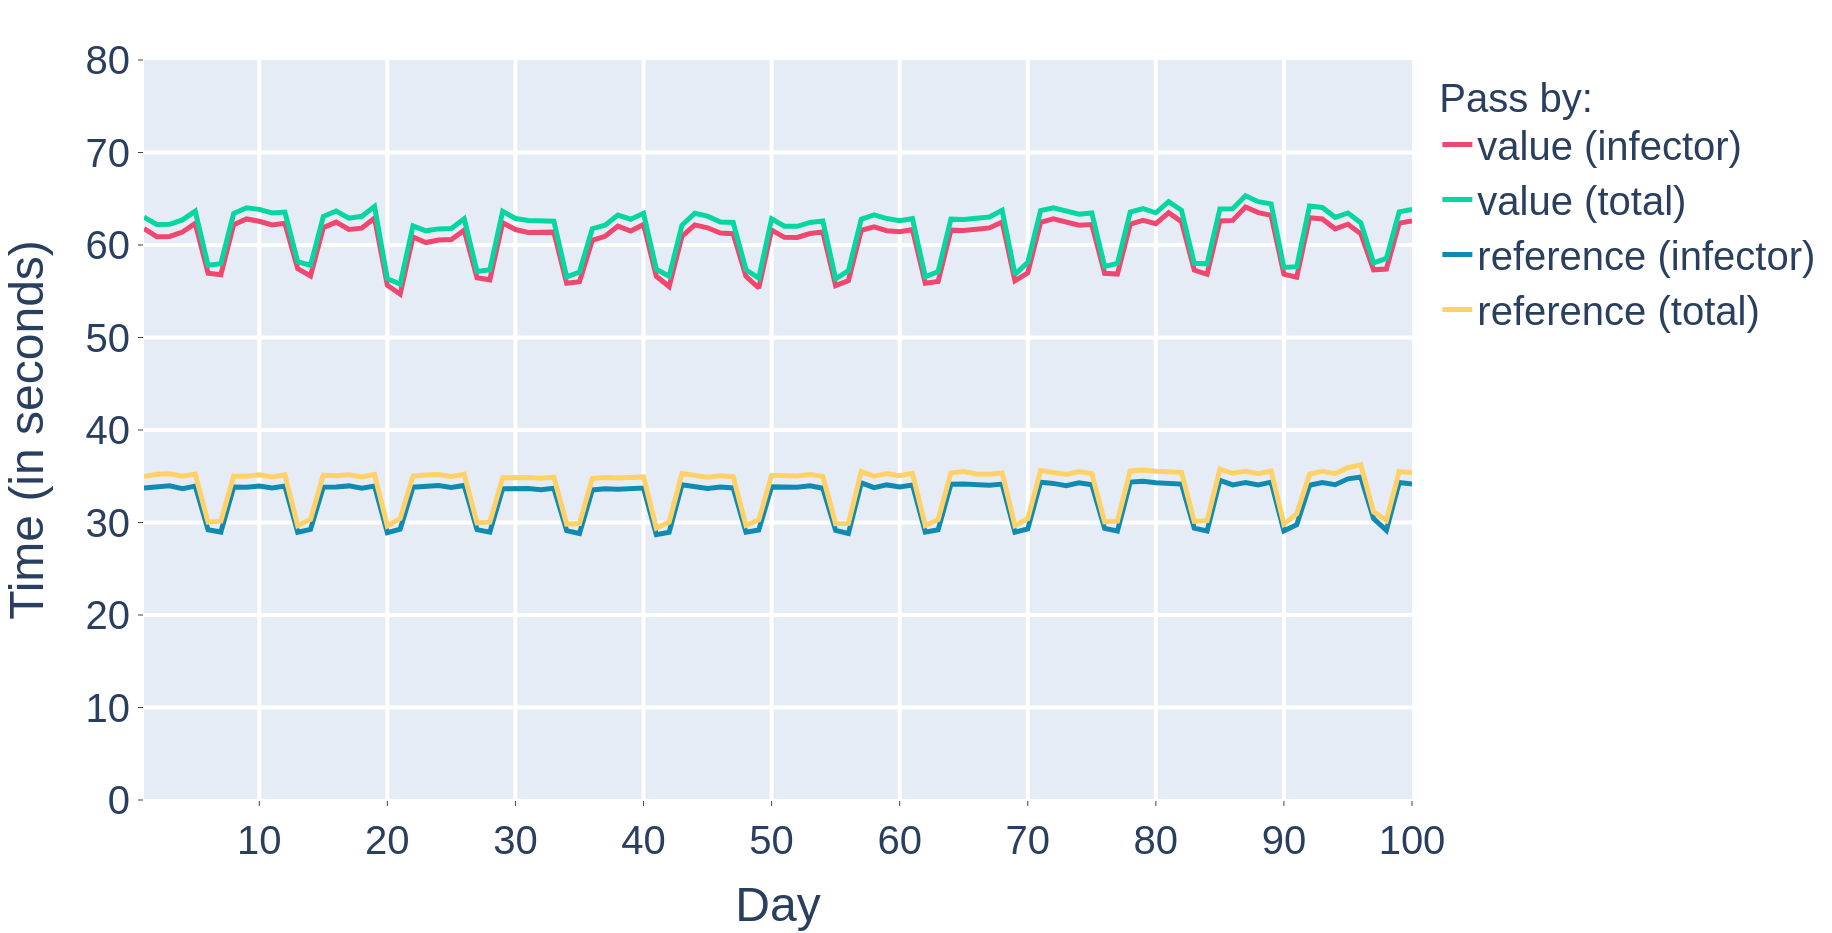
\includegraphics[width=\linewidth]{3 - Stride/fig/basis_standard_comparison_all.png}
        \caption{\textsc{All-to-All}}
        \label{fig:basis_standard_comparison_all}
    \end{subfigure}
    \begin{subfigure}[b]{\linewidth}
        \centering
        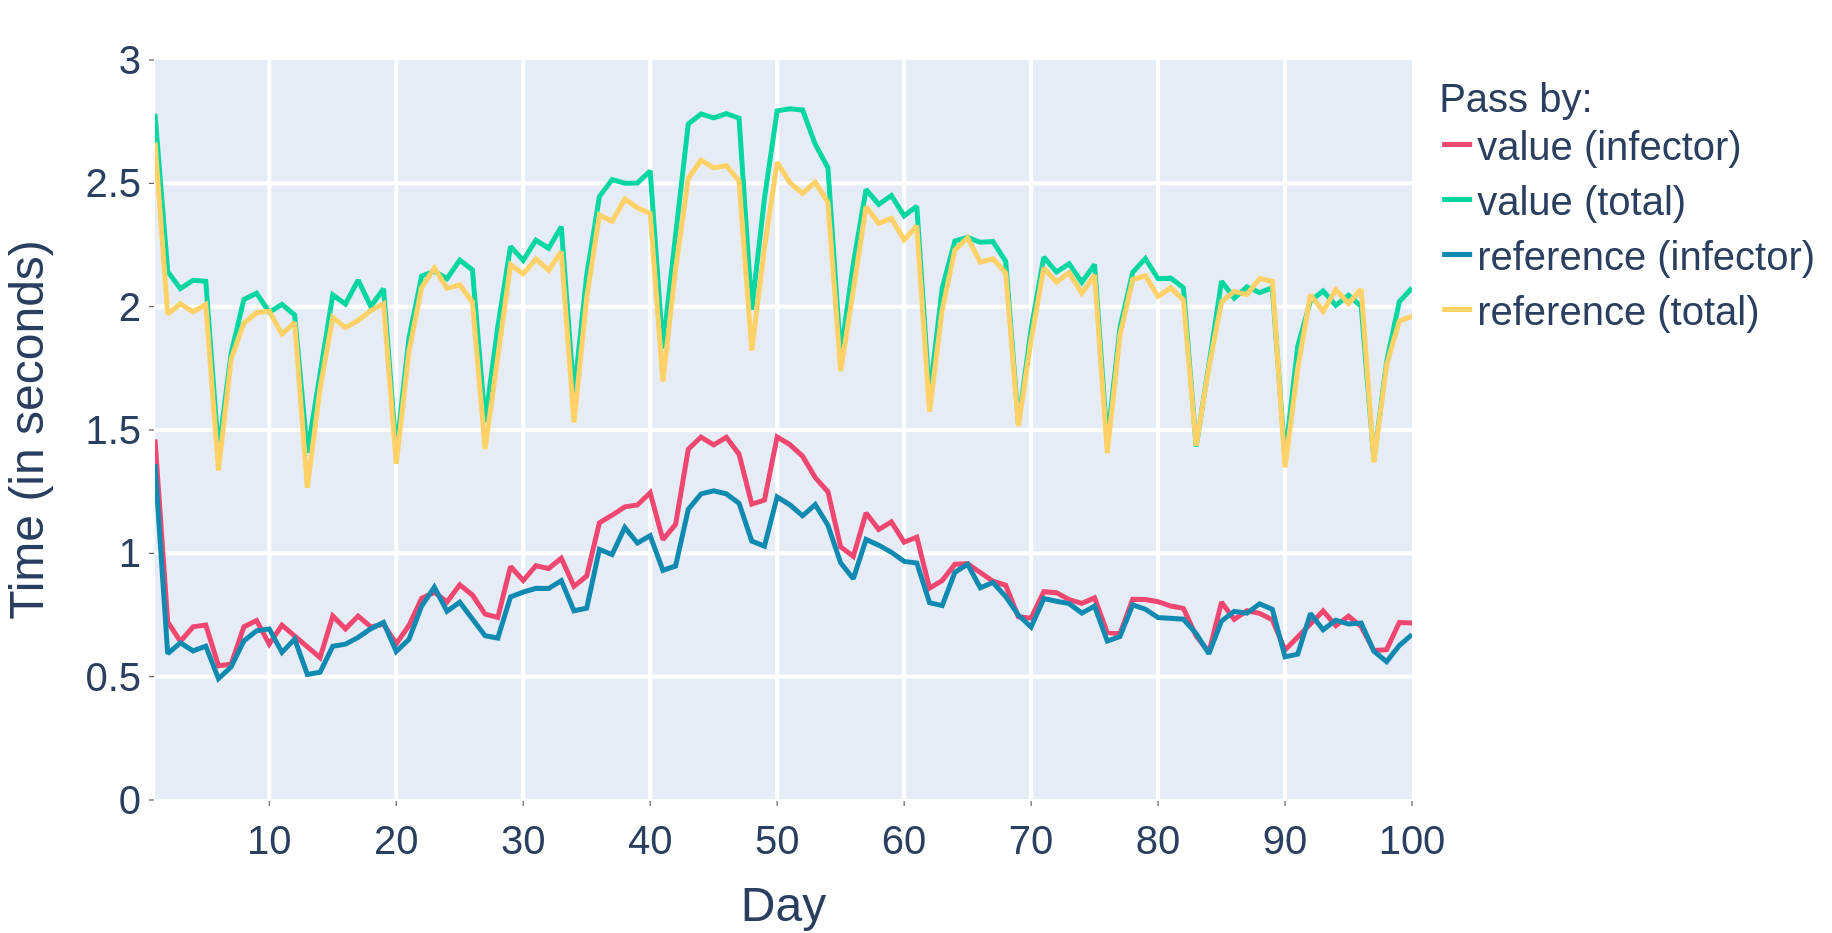
\includegraphics[width=\linewidth]{3 - Stride/fig/basis_standard_comparison_opt.png}
        \caption{\textsc{Inf-to-Sus}.}
        \label{fig:basis_standard_comparison_opt}
    \end{subfigure}
    \caption{Comparison of the infector and total runtimes of passing the population by value and by reference without parallellization. Simulations run on 11M population for 100 days without holidays using 1 thread (configurations in Appendix \ref{appendix:configurations}).}
    \label{fig:basis_standard_comparison}
\end{figure}

\begin{figure}
    \centering
    \begin{subfigure}[b]{\linewidth}
        \centering
        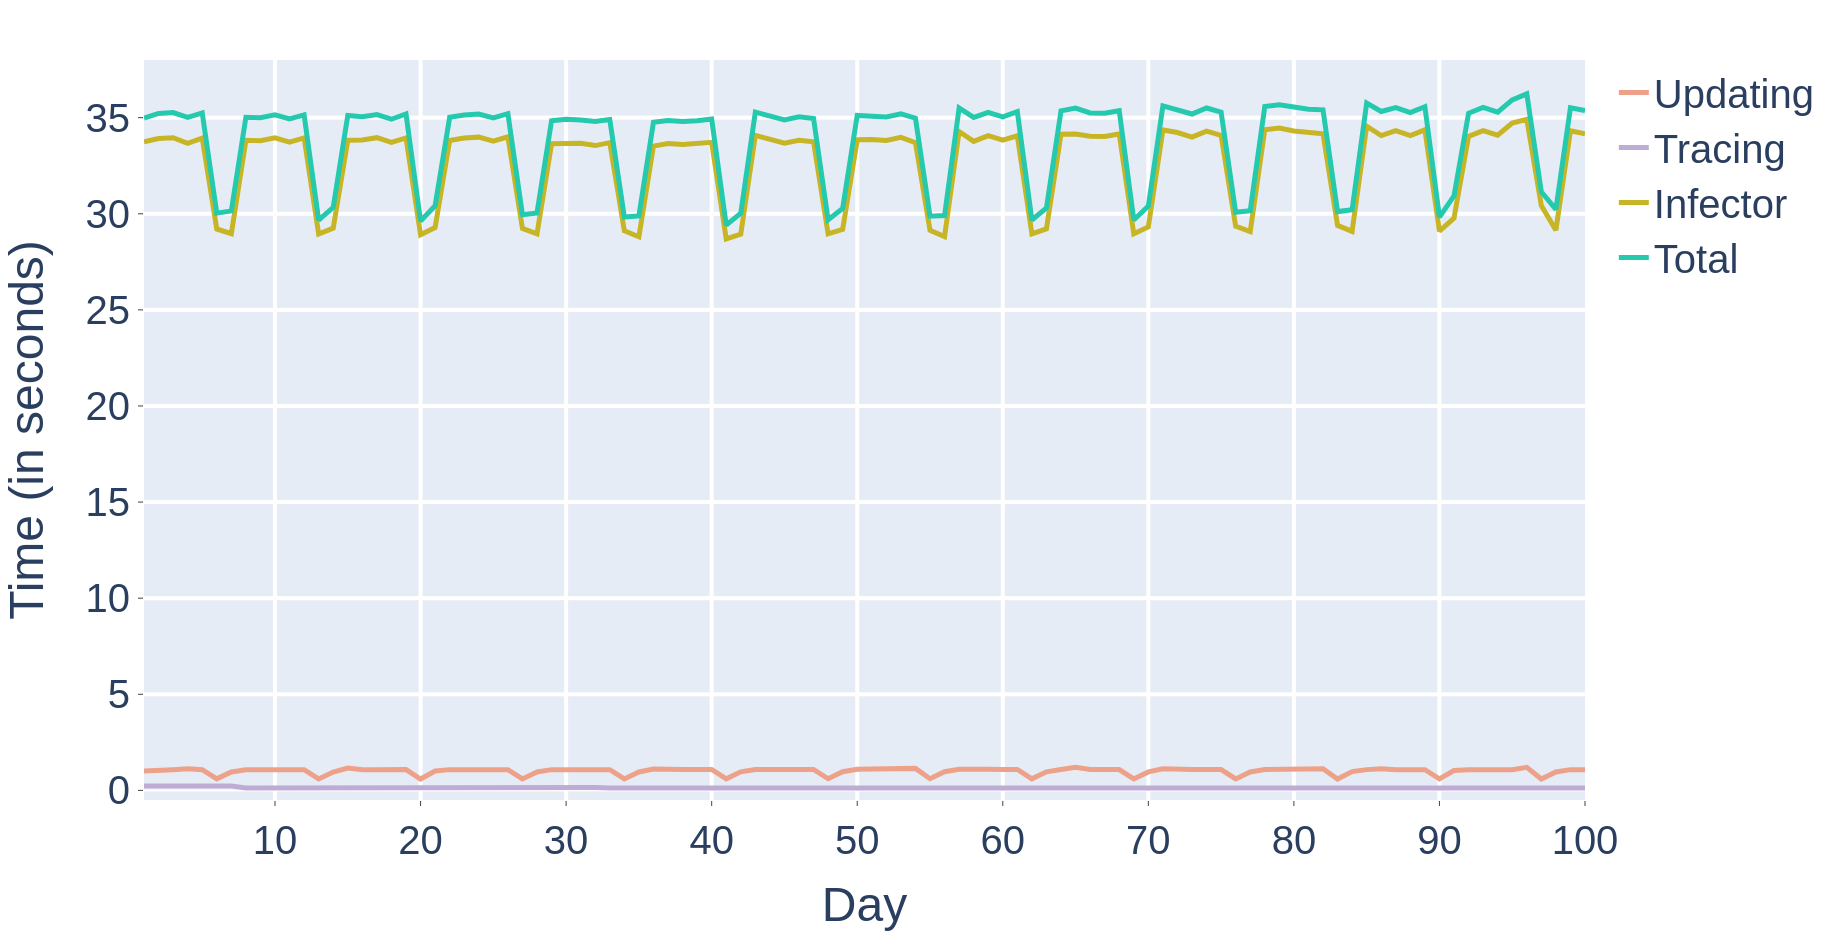
\includegraphics[width=\linewidth]{3 - Stride/fig/standard_all_runtime_sections.png}
        \caption{\textsc{All-to-All}}
        \label{fig:standard_all_sections}
    \end{subfigure}
    \begin{subfigure}[b]{\linewidth}
        \centering
        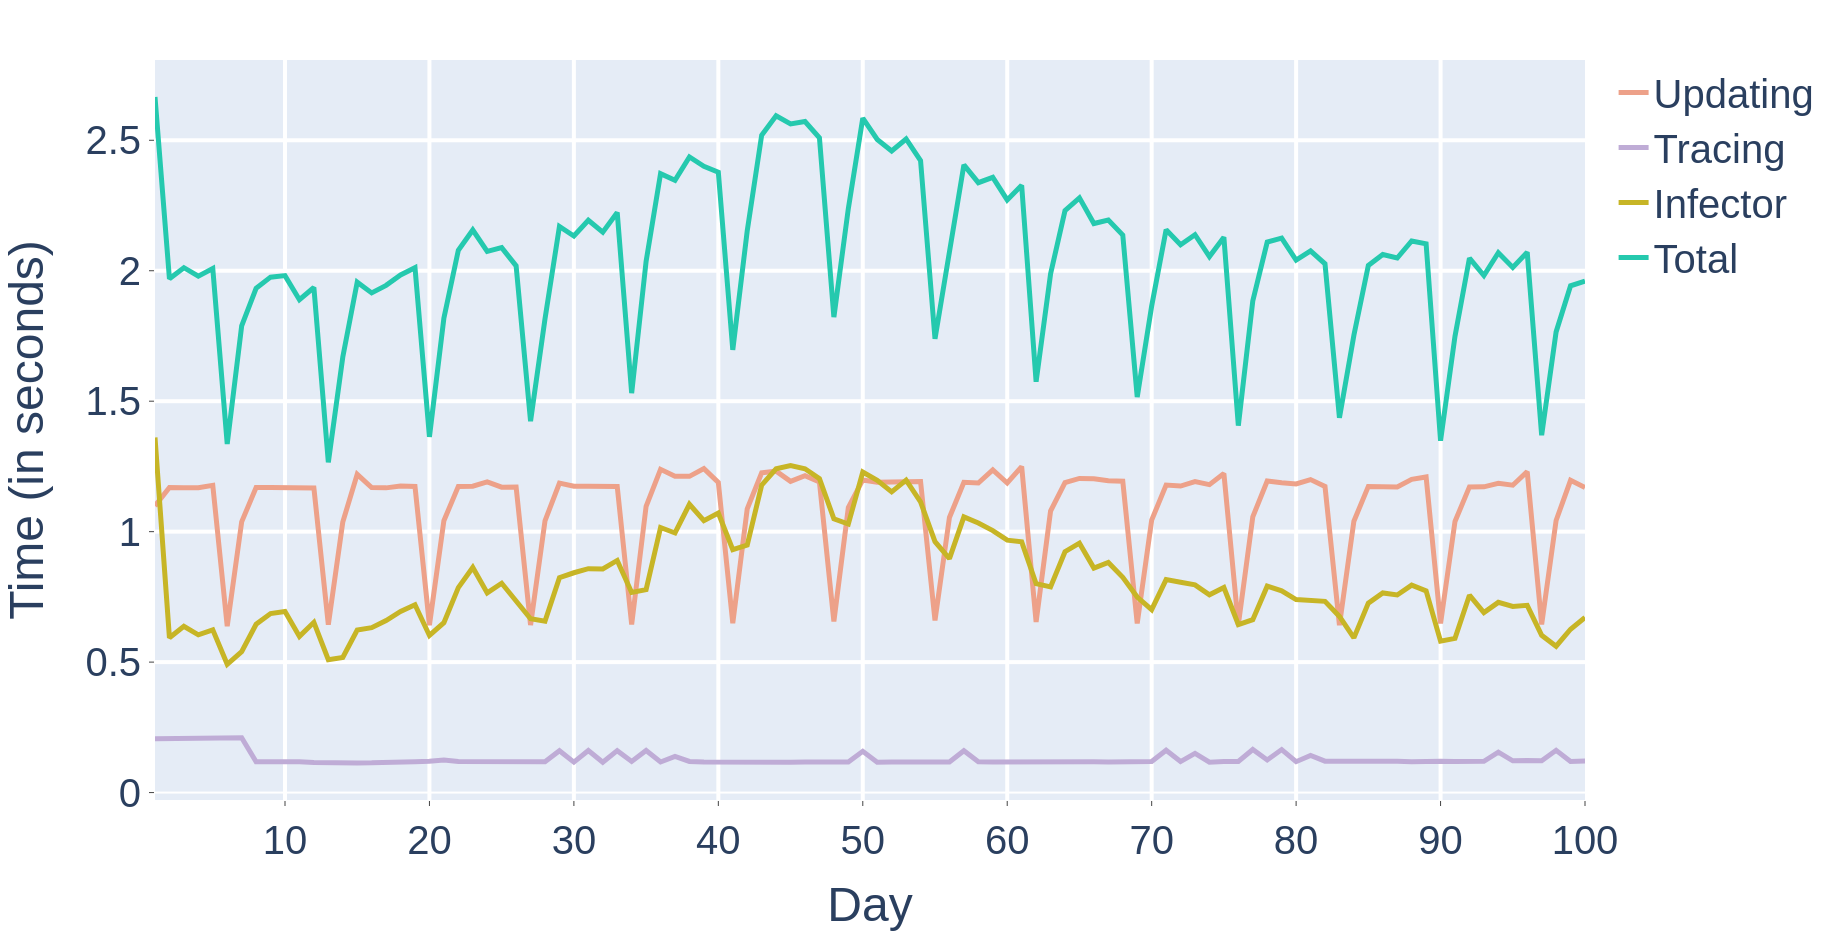
\includegraphics[width=\linewidth]{3 - Stride/fig/standard_opt_runtime_sections.png}
        \caption{\textsc{Inf-to-Sus}.}
        \label{fig:standard_opt_sections}
    \end{subfigure}
    \caption{Section times per day, in seconds, for every section, including the total times for simulating a day using the pass by reference optimisation. Simulations run on 11M population for 100 days without holidays using 1 thread (configurations in Appendix \ref{appendix:configurations}).}
    \label{fig:standard_sections}
\end{figure}

\begin{figure}
    \centering
    \begin{subfigure}[b]{\linewidth}
        \centering
        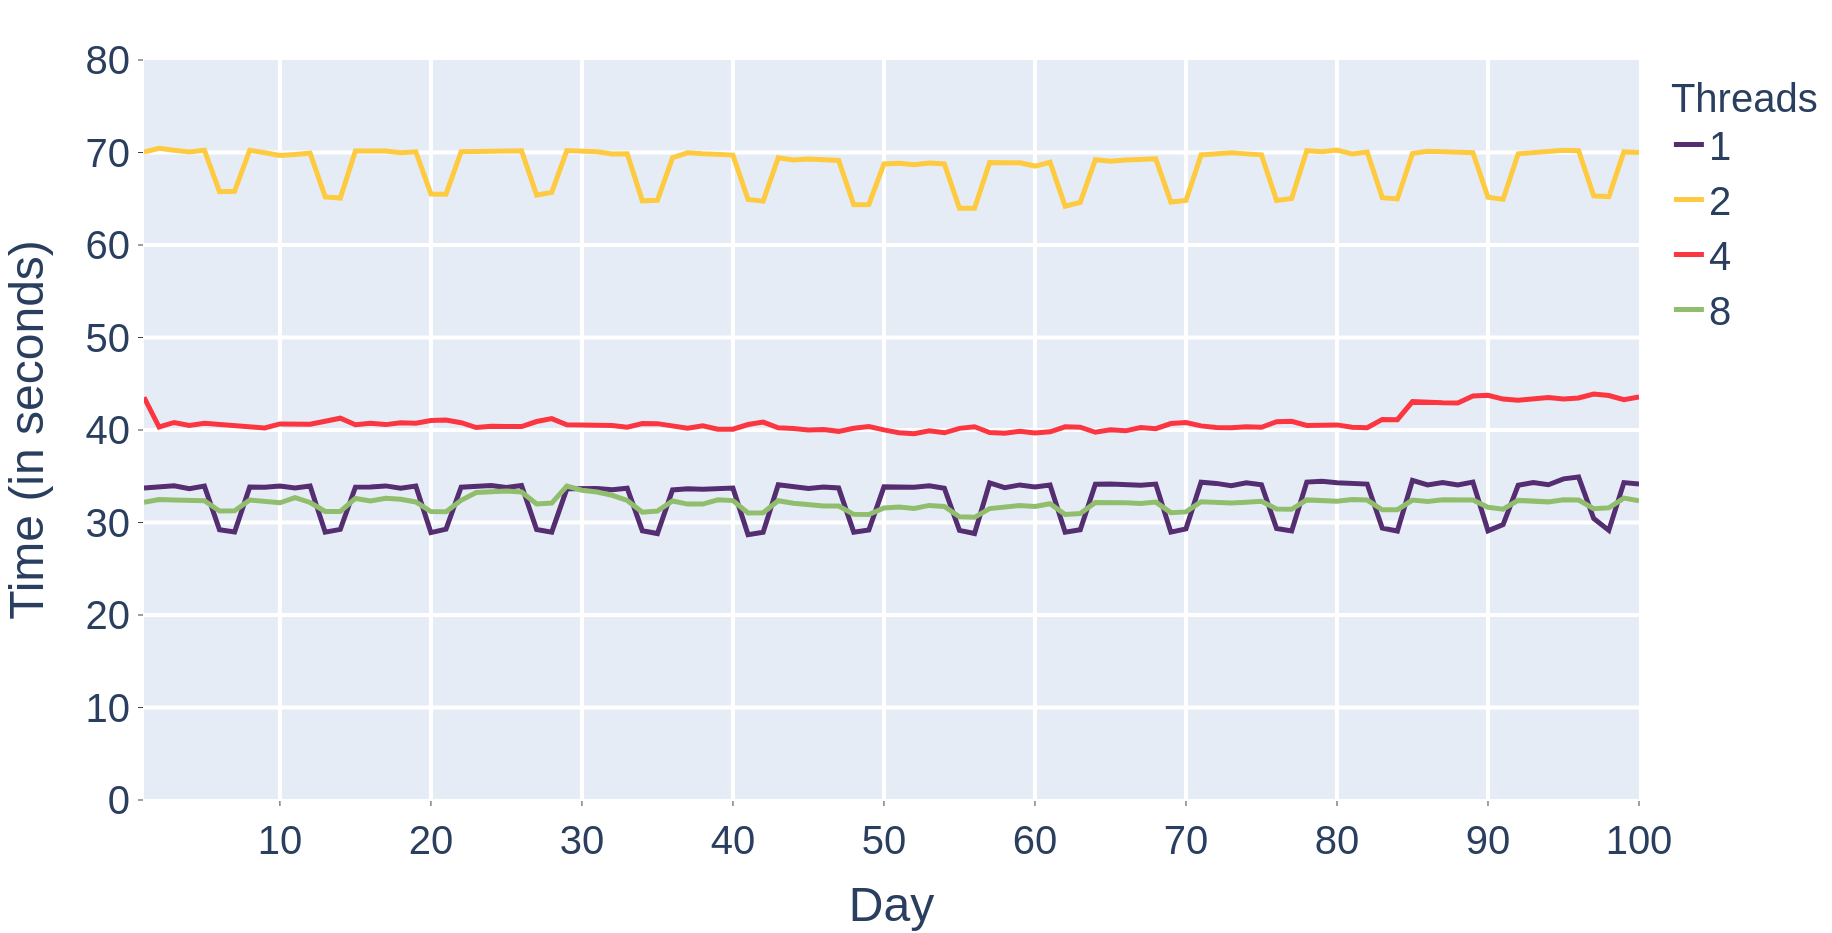
\includegraphics[width=\linewidth]{3 - Stride/fig/standard_all_parallel_infector.png}
        \caption{\textsc{All-to-All}}
        \label{fig:standard_all_parallel_infector}
    \end{subfigure}
    \begin{subfigure}[b]{\linewidth}
        \centering
        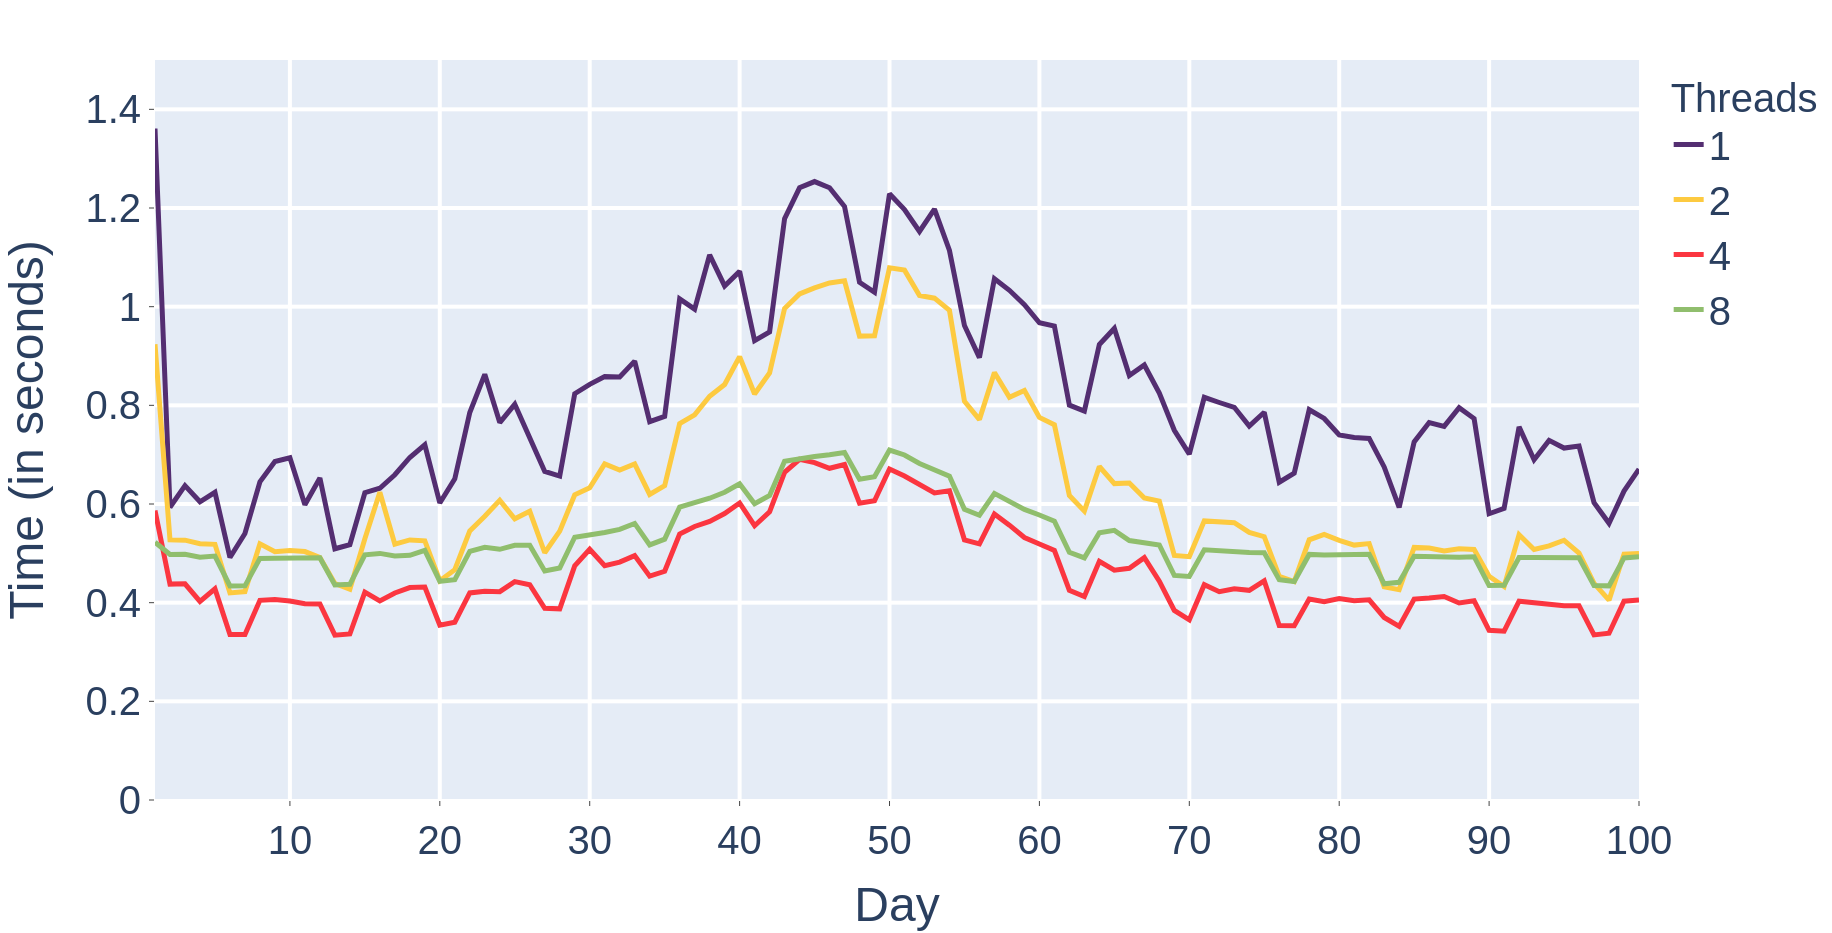
\includegraphics[width=\linewidth]{3 - Stride/fig/standard_opt_parallel_infector.png}
        \caption{\textsc{Inf-to-Sus}.}
        \label{fig:standard_opt_parallel_infector}
    \end{subfigure}
    \caption{Time per day for the infector that passes the $shared\_ptr$ population by reference, using different number of threads. Simulations run on 11M population for 100 days without holidays using 1 thread (configurations in Appendix \ref{appendix:configurations}).}
    \label{fig:standard_parallel_infector}
\end{figure}

\begin{table}[!ht]
    \begin{subtable}[h]{0.45\textwidth}
        \centering
        \begin{tabular}{@{}lrr@{}}
            \toprule
             & Infector & Total \\ \midrule
            pass by value & 60.37 & 61.52 \\
            pass by reference & 32.63 & 33.77 \\ \hdashline[1pt/1pt]
            speedup & 1.85 & 1.82 \\ \bottomrule
        \end{tabular}
        \caption{\textsc{All-to-All}}
        \label{tab:basis_standard_all}
    \end{subtable}
    \hfill
    \begin{subtable}[h]{0.45\textwidth}
        \centering
        \begin{tabular}{@{}lrr@{}}
            \toprule
             & Infector & Total \\ \midrule
            pass by value & 0.89 & 2.12 \\
            pass by reference & 0.82 & 2.04 \\ \hdashline[1pt/1pt]
            speedup & 1.09 & 1.04 \\ \bottomrule
        \end{tabular}
        \caption{\textsc{Inf-to-Sus}.}
        \label{tab:basis_standard_opt}
    \end{subtable}
    \caption{Average daily runtime (in seconds) per section of Stride before and after the optimisation with passing by reference. Simulations run on 11M population for 100 days without holidays using 1 thread (configurations in Appendix \ref{appendix:configurations}).}
    \label{tab:basis_standard}
\end{table}

\begin{table}[!ht]
\centering
\begin{tabular}{@{}lrrrr@{}}
\toprule
 & Updating & Tracing & Infector & Total \\ \midrule
All-to-All & 1.01 & 0.13 & 32.63 & 33.77 \\
Inf-to-Sus & 1.09 & 0.13 & 0.82 & 2.04 \\ \bottomrule
\end{tabular}
\caption{Average daily runtime (in seconds) per section of Stride with the passing by reference optimisation. Simulations run on 11M population for 100 days without holidays using 1 thread (configurations in Appendix \ref{appendix:configurations}).}
\label{tab:standard_sections}
\end{table}

\begin{table}[!ht]
    \begin{subtable}[h]{0.45\textwidth}
        \centering
        \begin{tabular}{@{}clrr@{}}
            \toprule
            Threads & Method & Infector & Total \\ \midrule
            \multirow{2}{*}{1} & by value & 60.37 & 61.52 \\
             & by reference & 32.63 & 33.77 \\ \hdashline[1pt/1pt]
             & speedup & 1.85 & 1.82 \\ \midrule
            \multirow{2}{*}{2} & by value & 227.93 & 229.50 \\
             & by reference & 68.40 & 70.13 \\ \hdashline[1pt/1pt]
             & speedup & 3.33 & 3.27 \\ \midrule
            \multirow{2}{*}{4} & by value & 197.04 & 198.85 \\
             & by reference & 40.91 & 42.68 \\ \hdashline[1pt/1pt]
             & speedup & 4.82 & 4.66 \\ \midrule
            \multirow{2}{*}{8} & by value & 187.15 & 189.00 \\
             & by reference & 32.03 & 33.82 \\ \hdashline[1pt/1pt]
             & speedup & 5.84 & 5.89 \\ \bottomrule
        \end{tabular}
    \caption{\textsc{All-to-All}}
    \label{tab:basis_standard_parallel_all}
    \end{subtable}
    \hfill
    \begin{subtable}[h]{0.45\textwidth}
        \centering
        \begin{tabular}{@{}clrr@{}}
            \toprule
            Threads & Method & Infector & Total \\ \midrule
            \multirow{2}{*}{1} & by value & 0.89 & 2.12 \\
             & by reference & 0.82 & 2.04 \\ \hdashline[1pt/1pt]
             & speedup & 1.09 & 1.04 \\ \midrule
            \multirow{2}{*}{2} & by value & 0.83 & 2.48 \\
             & by reference & 0.63 & 2.43 \\ \hdashline[1pt/1pt]
             & speedup & 1.32 & 1.02 \\ \midrule
            \multirow{2}{*}{4} & by value & 0.69 & 2.49 \\
             & by reference & 0.46 & 2.24 \\ \hdashline[1pt/1pt]
             & speedup & 1.50 & 1.11 \\ \midrule
            \multirow{2}{*}{8} & by value & 0.76 & 2.57 \\
             & by reference & 0.53 & 2.33 \\ \hdashline[1pt/1pt]
             & speedup & 1.43 & 1.10 \\ \bottomrule
        \end{tabular}
        \caption{\textsc{Inf-to-Sus}.}
        \label{tab:basis_standard_parallel_opt}
    \end{subtable}
    \caption{Comparison of the average daily runtimes (in seconds) per section before and after the pass by reference optimisation, depending on the number of used threads.  Simulations run on 11M population for 100 days without holidays (configurations in Appendix \ref{appendix:configurations}).}
    \label{tab:basis_standard_parallel}
\end{table}